\documentclass[twoside]{book}

% Packages required by doxygen
\usepackage{fixltx2e}
\usepackage{calc}
\usepackage{doxygen}
\usepackage[export]{adjustbox} % also loads graphicx
\usepackage{graphicx}
\usepackage[utf8]{inputenc}
\usepackage{makeidx}
\usepackage{multicol}
\usepackage{multirow}
\PassOptionsToPackage{warn}{textcomp}
\usepackage{textcomp}
\usepackage[nointegrals]{wasysym}
\usepackage[table]{xcolor}

% Font selection
\usepackage[T1]{fontenc}
\usepackage[scaled=.90]{helvet}
\usepackage{courier}
\usepackage{amssymb}
\usepackage{sectsty}
\renewcommand{\familydefault}{\sfdefault}
\allsectionsfont{%
  \fontseries{bc}\selectfont%
  \color{darkgray}%
}
\renewcommand{\DoxyLabelFont}{%
  \fontseries{bc}\selectfont%
  \color{darkgray}%
}
\newcommand{\+}{\discretionary{\mbox{\scriptsize$\hookleftarrow$}}{}{}}

% Page & text layout
\usepackage{geometry}
\geometry{%
  a4paper,%
  top=2.5cm,%
  bottom=2.5cm,%
  left=2.5cm,%
  right=2.5cm%
}
\tolerance=750
\hfuzz=15pt
\hbadness=750
\setlength{\emergencystretch}{15pt}
\setlength{\parindent}{0cm}
\setlength{\parskip}{3ex plus 2ex minus 2ex}
\makeatletter
\renewcommand{\paragraph}{%
  \@startsection{paragraph}{4}{0ex}{-1.0ex}{1.0ex}{%
    \normalfont\normalsize\bfseries\SS@parafont%
  }%
}
\renewcommand{\subparagraph}{%
  \@startsection{subparagraph}{5}{0ex}{-1.0ex}{1.0ex}{%
    \normalfont\normalsize\bfseries\SS@subparafont%
  }%
}
\makeatother

% Headers & footers
\usepackage{fancyhdr}
\pagestyle{fancyplain}
\fancyhead[LE]{\fancyplain{}{\bfseries\thepage}}
\fancyhead[CE]{\fancyplain{}{}}
\fancyhead[RE]{\fancyplain{}{\bfseries\leftmark}}
\fancyhead[LO]{\fancyplain{}{\bfseries\rightmark}}
\fancyhead[CO]{\fancyplain{}{}}
\fancyhead[RO]{\fancyplain{}{\bfseries\thepage}}
\fancyfoot[LE]{\fancyplain{}{}}
\fancyfoot[CE]{\fancyplain{}{}}
\fancyfoot[RE]{\fancyplain{}{\bfseries\scriptsize Generated by Doxygen }}
\fancyfoot[LO]{\fancyplain{}{\bfseries\scriptsize Generated by Doxygen }}
\fancyfoot[CO]{\fancyplain{}{}}
\fancyfoot[RO]{\fancyplain{}{}}
\renewcommand{\footrulewidth}{0.4pt}
\renewcommand{\chaptermark}[1]{%
  \markboth{#1}{}%
}
\renewcommand{\sectionmark}[1]{%
  \markright{\thesection\ #1}%
}

% Indices & bibliography
\usepackage{natbib}
\usepackage[titles]{tocloft}
\setcounter{tocdepth}{3}
\setcounter{secnumdepth}{5}
\makeindex

% Hyperlinks (required, but should be loaded last)
\usepackage{ifpdf}
\ifpdf
  \usepackage[pdftex,pagebackref=true]{hyperref}
\else
  \usepackage[ps2pdf,pagebackref=true]{hyperref}
\fi
\hypersetup{%
  colorlinks=true,%
  linkcolor=blue,%
  citecolor=blue,%
  unicode%
}

% Custom commands
\newcommand{\clearemptydoublepage}{%
  \newpage{\pagestyle{empty}\cleardoublepage}%
}

\usepackage{caption}
\captionsetup{labelsep=space,justification=centering,font={bf},singlelinecheck=off,skip=4pt,position=top}

%===== C O N T E N T S =====

\begin{document}

% Titlepage & ToC
\hypersetup{pageanchor=false,
             bookmarksnumbered=true,
             pdfencoding=unicode
            }
\pagenumbering{alph}
\begin{titlepage}
\vspace*{7cm}
\begin{center}%
{\Large Semestralka }\\
\vspace*{1cm}
{\large Generated by Doxygen 1.8.14}\\
\end{center}
\end{titlepage}
\clearemptydoublepage
\pagenumbering{roman}
\tableofcontents
\clearemptydoublepage
\pagenumbering{arabic}
\hypersetup{pageanchor=true}

%--- Begin generated contents ---
\chapter{Hierarchical Index}
\section{Class Hierarchy}
This inheritance list is sorted roughly, but not completely, alphabetically\+:\begin{DoxyCompactList}
\item \contentsline{section}{C\+Calendar}{\pageref{class_c_calendar}}{}
\item \contentsline{section}{C\+Calendar\+Export\+Base}{\pageref{class_c_calendar_export_base}}{}
\item \contentsline{section}{C\+Command\+Interpreter}{\pageref{class_c_command_interpreter}}{}
\item \contentsline{section}{C\+Date}{\pageref{class_c_date}}{}
\item \contentsline{section}{C\+Duration}{\pageref{class_c_duration}}{}
\item \contentsline{section}{C\+Event}{\pageref{class_c_event}}{}
\item \contentsline{section}{C\+Event\+Repeat\+Base}{\pageref{class_c_event_repeat_base}}{}
\begin{DoxyCompactList}
\item \contentsline{section}{C\+Event\+Repeat\+After}{\pageref{class_c_event_repeat_after}}{}
\item \contentsline{section}{C\+Event\+Repeat\+Day\+In\+Month}{\pageref{class_c_event_repeat_day_in_month}}{}
\item \contentsline{section}{C\+Event\+Repeat\+Disabled}{\pageref{class_c_event_repeat_disabled}}{}
\end{DoxyCompactList}
\item \contentsline{section}{C\+Event\+Transfer\+Base}{\pageref{class_c_event_transfer_base}}{}
\begin{DoxyCompactList}
\item \contentsline{section}{C\+Event\+Transfer\+Disabled}{\pageref{class_c_event_transfer_disabled}}{}
\end{DoxyCompactList}
\item \contentsline{section}{C\+I\+D\+Extractor$<$ T $>$}{\pageref{struct_c_i_d_extractor}}{}
\item \contentsline{section}{C\+Suggestor$<$ T, Extractor $>$}{\pageref{class_c_suggestor}}{}
\item \contentsline{section}{C\+Suggestor$<$ C\+Event $\ast$, C\+Event\+:\+:Get\+Searchable $>$}{\pageref{class_c_suggestor}}{}
\item \contentsline{section}{C\+View\+Base}{\pageref{class_c_view_base}}{}
\begin{DoxyCompactList}
\item \contentsline{section}{C\+View\+Month}{\pageref{class_c_view_month}}{}
\item \contentsline{section}{C\+View\+Week}{\pageref{class_c_view_week}}{}
\item \contentsline{section}{C\+View\+Year}{\pageref{class_c_view_year}}{}
\end{DoxyCompactList}
\item \contentsline{section}{C\+View\+Day}{\pageref{class_c_view_day}}{}
\item \contentsline{section}{Empty\+Line\+Exception}{\pageref{class_empty_line_exception}}{}
\item \contentsline{section}{C\+Event\+:\+:Get\+Searchable}{\pageref{struct_c_event_1_1_get_searchable}}{}
\item \contentsline{section}{C\+Duration\+:\+:Separated}{\pageref{struct_c_duration_1_1_separated}}{}
\end{DoxyCompactList}

\chapter{Class Index}
\section{Class List}
Here are the classes, structs, unions and interfaces with brief descriptions\+:\begin{DoxyCompactList}
\item\contentsline{section}{\mbox{\hyperlink{class_c_calendar}{C\+Calendar}} }{\pageref{class_c_calendar}}{}
\item\contentsline{section}{\mbox{\hyperlink{class_c_calendar_export_base}{C\+Calendar\+Export\+Base}} }{\pageref{class_c_calendar_export_base}}{}
\item\contentsline{section}{\mbox{\hyperlink{class_c_command_interpreter}{C\+Command\+Interpreter}} }{\pageref{class_c_command_interpreter}}{}
\item\contentsline{section}{\mbox{\hyperlink{class_c_date}{C\+Date}} }{\pageref{class_c_date}}{}
\item\contentsline{section}{\mbox{\hyperlink{class_c_duration}{C\+Duration}} }{\pageref{class_c_duration}}{}
\item\contentsline{section}{\mbox{\hyperlink{class_c_event}{C\+Event}} }{\pageref{class_c_event}}{}
\item\contentsline{section}{\mbox{\hyperlink{class_c_event_repeat_after}{C\+Event\+Repeat\+After}} }{\pageref{class_c_event_repeat_after}}{}
\item\contentsline{section}{\mbox{\hyperlink{class_c_event_repeat_base}{C\+Event\+Repeat\+Base}} }{\pageref{class_c_event_repeat_base}}{}
\item\contentsline{section}{\mbox{\hyperlink{class_c_event_repeat_day_in_month}{C\+Event\+Repeat\+Day\+In\+Month}} }{\pageref{class_c_event_repeat_day_in_month}}{}
\item\contentsline{section}{\mbox{\hyperlink{class_c_event_repeat_disabled}{C\+Event\+Repeat\+Disabled}} }{\pageref{class_c_event_repeat_disabled}}{}
\item\contentsline{section}{\mbox{\hyperlink{class_c_event_transfer_base}{C\+Event\+Transfer\+Base}} }{\pageref{class_c_event_transfer_base}}{}
\item\contentsline{section}{\mbox{\hyperlink{class_c_event_transfer_disabled}{C\+Event\+Transfer\+Disabled}} }{\pageref{class_c_event_transfer_disabled}}{}
\item\contentsline{section}{\mbox{\hyperlink{struct_c_i_d_extractor}{C\+I\+D\+Extractor$<$ T $>$}} }{\pageref{struct_c_i_d_extractor}}{}
\item\contentsline{section}{\mbox{\hyperlink{class_c_suggestor}{C\+Suggestor$<$ T, Extractor $>$}} }{\pageref{class_c_suggestor}}{}
\item\contentsline{section}{\mbox{\hyperlink{class_c_view_base}{C\+View\+Base}} }{\pageref{class_c_view_base}}{}
\item\contentsline{section}{\mbox{\hyperlink{class_c_view_day}{C\+View\+Day}} }{\pageref{class_c_view_day}}{}
\item\contentsline{section}{\mbox{\hyperlink{class_c_view_month}{C\+View\+Month}} }{\pageref{class_c_view_month}}{}
\item\contentsline{section}{\mbox{\hyperlink{class_c_view_week}{C\+View\+Week}} }{\pageref{class_c_view_week}}{}
\item\contentsline{section}{\mbox{\hyperlink{class_c_view_year}{C\+View\+Year}} }{\pageref{class_c_view_year}}{}
\item\contentsline{section}{\mbox{\hyperlink{class_empty_line_exception}{Empty\+Line\+Exception}} }{\pageref{class_empty_line_exception}}{}
\item\contentsline{section}{\mbox{\hyperlink{struct_c_event_1_1_get_searchable}{C\+Event\+::\+Get\+Searchable}} }{\pageref{struct_c_event_1_1_get_searchable}}{}
\item\contentsline{section}{\mbox{\hyperlink{struct_c_duration_1_1_separated}{C\+Duration\+::\+Separated}} }{\pageref{struct_c_duration_1_1_separated}}{}
\end{DoxyCompactList}

\chapter{File Index}
\section{File List}
Here is a list of all files with brief descriptions\+:\begin{DoxyCompactList}
\item\contentsline{section}{\mbox{\hyperlink{main_8cpp}{main.\+cpp}} }{\pageref{main_8cpp}}{}
\item\contentsline{section}{Calendar/\mbox{\hyperlink{_c_calendar_8cpp}{C\+Calendar.\+cpp}} }{\pageref{_c_calendar_8cpp}}{}
\item\contentsline{section}{Calendar/\mbox{\hyperlink{_c_calendar_8h}{C\+Calendar.\+h}} }{\pageref{_c_calendar_8h}}{}
\item\contentsline{section}{cmake-\/build-\/debug/\+C\+Make\+Files/\mbox{\hyperlink{feature__tests_8c}{feature\+\_\+tests.\+c}} }{\pageref{feature__tests_8c}}{}
\item\contentsline{section}{cmake-\/build-\/debug/\+C\+Make\+Files/\mbox{\hyperlink{feature__tests_8cxx}{feature\+\_\+tests.\+cxx}} }{\pageref{feature__tests_8cxx}}{}
\item\contentsline{section}{cmake-\/build-\/debug/\+C\+Make\+Files/3.\+8.\+2/\+Compiler\+Id\+C/\mbox{\hyperlink{_c_make_c_compiler_id_8c}{C\+Make\+C\+Compiler\+Id.\+c}} }{\pageref{_c_make_c_compiler_id_8c}}{}
\item\contentsline{section}{cmake-\/build-\/debug/\+C\+Make\+Files/3.\+8.\+2/\+Compiler\+Id\+C\+X\+X/\mbox{\hyperlink{_c_make_c_x_x_compiler_id_8cpp}{C\+Make\+C\+X\+X\+Compiler\+Id.\+cpp}} }{\pageref{_c_make_c_x_x_compiler_id_8cpp}}{}
\item\contentsline{section}{Date/\mbox{\hyperlink{_c_date_8cpp}{C\+Date.\+cpp}} }{\pageref{_c_date_8cpp}}{}
\item\contentsline{section}{Date/\mbox{\hyperlink{_c_date_8h}{C\+Date.\+h}} }{\pageref{_c_date_8h}}{}
\item\contentsline{section}{Date/\mbox{\hyperlink{_c_duration_8cpp}{C\+Duration.\+cpp}} }{\pageref{_c_duration_8cpp}}{}
\item\contentsline{section}{Date/\mbox{\hyperlink{_c_duration_8h}{C\+Duration.\+h}} }{\pageref{_c_duration_8h}}{}
\item\contentsline{section}{Event/\mbox{\hyperlink{_c_event_8cpp}{C\+Event.\+cpp}} }{\pageref{_c_event_8cpp}}{}
\item\contentsline{section}{Event/\mbox{\hyperlink{_c_event_8h}{C\+Event.\+h}} }{\pageref{_c_event_8h}}{}
\item\contentsline{section}{Exporters/\mbox{\hyperlink{_c_calendar_export_base_8h}{C\+Calendar\+Export\+Base.\+h}} }{\pageref{_c_calendar_export_base_8h}}{}
\item\contentsline{section}{Repeat\+Strategies/\mbox{\hyperlink{_c_event_repeat_after_8cpp}{C\+Event\+Repeat\+After.\+cpp}} }{\pageref{_c_event_repeat_after_8cpp}}{}
\item\contentsline{section}{Repeat\+Strategies/\mbox{\hyperlink{_c_event_repeat_after_8h}{C\+Event\+Repeat\+After.\+h}} }{\pageref{_c_event_repeat_after_8h}}{}
\item\contentsline{section}{Repeat\+Strategies/\mbox{\hyperlink{_c_event_repeat_base_8cpp}{C\+Event\+Repeat\+Base.\+cpp}} }{\pageref{_c_event_repeat_base_8cpp}}{}
\item\contentsline{section}{Repeat\+Strategies/\mbox{\hyperlink{_c_event_repeat_base_8h}{C\+Event\+Repeat\+Base.\+h}} }{\pageref{_c_event_repeat_base_8h}}{}
\item\contentsline{section}{Repeat\+Strategies/\mbox{\hyperlink{_c_event_repeat_day_in_month_8cpp}{C\+Event\+Repeat\+Day\+In\+Month.\+cpp}} }{\pageref{_c_event_repeat_day_in_month_8cpp}}{}
\item\contentsline{section}{Repeat\+Strategies/\mbox{\hyperlink{_c_event_repeat_day_in_month_8h}{C\+Event\+Repeat\+Day\+In\+Month.\+h}} }{\pageref{_c_event_repeat_day_in_month_8h}}{}
\item\contentsline{section}{Repeat\+Strategies/\mbox{\hyperlink{_c_event_repeat_disabled_8cpp}{C\+Event\+Repeat\+Disabled.\+cpp}} }{\pageref{_c_event_repeat_disabled_8cpp}}{}
\item\contentsline{section}{Repeat\+Strategies/\mbox{\hyperlink{_c_event_repeat_disabled_8h}{C\+Event\+Repeat\+Disabled.\+h}} }{\pageref{_c_event_repeat_disabled_8h}}{}
\item\contentsline{section}{Transfer\+Strategies/\mbox{\hyperlink{_c_event_transfer_base_8h}{C\+Event\+Transfer\+Base.\+h}} }{\pageref{_c_event_transfer_base_8h}}{}
\item\contentsline{section}{Transfer\+Strategies/\mbox{\hyperlink{_c_event_transfer_disabled_8cpp}{C\+Event\+Transfer\+Disabled.\+cpp}} }{\pageref{_c_event_transfer_disabled_8cpp}}{}
\item\contentsline{section}{Transfer\+Strategies/\mbox{\hyperlink{_c_event_transfer_disabled_8h}{C\+Event\+Transfer\+Disabled.\+h}} }{\pageref{_c_event_transfer_disabled_8h}}{}
\item\contentsline{section}{U\+I/\mbox{\hyperlink{_c_command_interpreter_8cpp}{C\+Command\+Interpreter.\+cpp}} }{\pageref{_c_command_interpreter_8cpp}}{}
\item\contentsline{section}{U\+I/\mbox{\hyperlink{_c_command_interpreter_8h}{C\+Command\+Interpreter.\+h}} }{\pageref{_c_command_interpreter_8h}}{}
\item\contentsline{section}{U\+I/\mbox{\hyperlink{_c_view_base_8cpp}{C\+View\+Base.\+cpp}} }{\pageref{_c_view_base_8cpp}}{}
\item\contentsline{section}{U\+I/\mbox{\hyperlink{_c_view_base_8h}{C\+View\+Base.\+h}} }{\pageref{_c_view_base_8h}}{}
\item\contentsline{section}{U\+I/\mbox{\hyperlink{_c_view_day_8cpp}{C\+View\+Day.\+cpp}} }{\pageref{_c_view_day_8cpp}}{}
\item\contentsline{section}{U\+I/\mbox{\hyperlink{_c_view_day_8h}{C\+View\+Day.\+h}} }{\pageref{_c_view_day_8h}}{}
\item\contentsline{section}{U\+I/\mbox{\hyperlink{_c_view_month_8cpp}{C\+View\+Month.\+cpp}} }{\pageref{_c_view_month_8cpp}}{}
\item\contentsline{section}{U\+I/\mbox{\hyperlink{_c_view_month_8h}{C\+View\+Month.\+h}} }{\pageref{_c_view_month_8h}}{}
\item\contentsline{section}{U\+I/\mbox{\hyperlink{_c_view_week_8cpp}{C\+View\+Week.\+cpp}} }{\pageref{_c_view_week_8cpp}}{}
\item\contentsline{section}{U\+I/\mbox{\hyperlink{_c_view_week_8h}{C\+View\+Week.\+h}} }{\pageref{_c_view_week_8h}}{}
\item\contentsline{section}{U\+I/\mbox{\hyperlink{_c_view_year_8cpp}{C\+View\+Year.\+cpp}} }{\pageref{_c_view_year_8cpp}}{}
\item\contentsline{section}{U\+I/\mbox{\hyperlink{_c_view_year_8h}{C\+View\+Year.\+h}} }{\pageref{_c_view_year_8h}}{}
\item\contentsline{section}{utils/\mbox{\hyperlink{_c_suggestor_8h}{C\+Suggestor.\+h}} }{\pageref{_c_suggestor_8h}}{}
\item\contentsline{section}{utils/\mbox{\hyperlink{utils_8cpp}{utils.\+cpp}} }{\pageref{utils_8cpp}}{}
\item\contentsline{section}{utils/\mbox{\hyperlink{utils_8h}{utils.\+h}} }{\pageref{utils_8h}}{}
\end{DoxyCompactList}

\chapter{Class Documentation}
\hypertarget{class_c_calendar}{}\section{C\+Calendar Class Reference}
\label{class_c_calendar}\index{C\+Calendar@{C\+Calendar}}


{\ttfamily \#include $<$C\+Calendar.\+h$>$}

\subsection*{Public Member Functions}
\begin{DoxyCompactItemize}
\item 
\mbox{\hyperlink{class_c_calendar_aa3fe418a1d8f93508047f923eb229b56}{C\+Calendar}} ()
\item 
\mbox{\hyperlink{class_c_calendar_af0c5cbee7d55fefa23f340cecbd45ec9}{$\sim$\+C\+Calendar}} ()
\item 
void \mbox{\hyperlink{class_c_calendar_a8ab0b10b7e49fd718224e982009a2d5d}{Add\+Event}} (\mbox{\hyperlink{class_c_event}{C\+Event}} $\ast$ev)
\item 
void \mbox{\hyperlink{class_c_calendar_a07b2bad77df73457a930c9df19ef1719}{Create\+Event}} ()
\item 
std\+::map$<$ int, \mbox{\hyperlink{class_c_event}{C\+Event}} $\ast$ $>$\+::const\+\_\+iterator \mbox{\hyperlink{class_c_calendar_abdb8378eabf26455d239222e66f73976}{Find\+Event}} (int ID) const
\item 
void \mbox{\hyperlink{class_c_calendar_a34a4175ed902ac35803f45a39b7dfc97}{Remove\+Event}} (const std\+::map$<$ int, \mbox{\hyperlink{class_c_event}{C\+Event}} $\ast$$>$\+::const\+\_\+iterator \&it)
\item 
void \mbox{\hyperlink{class_c_calendar_aa3fe3ae0f796ea634ba5a52bf1fb5018}{Remove\+Event}} (int ID)
\item 
void \mbox{\hyperlink{class_c_calendar_a4563ae3538b60e88bb3a80d9f9638656}{Edit\+Event}} (const std\+::map$<$ int, \mbox{\hyperlink{class_c_event}{C\+Event}} $\ast$$>$\+::const\+\_\+iterator \&it)
\item 
void \mbox{\hyperlink{class_c_calendar_af881187353fc545c859db39e39d7ec71}{Edit\+Event}} (int ID)
\item 
std\+::map$<$ \mbox{\hyperlink{class_c_date_af23472c977b14ed341b48183ec19d874}{C\+Date\+::\+Interval}}, \mbox{\hyperlink{class_c_event}{C\+Event}} $\ast$ $>$ \mbox{\hyperlink{class_c_calendar_a0aef6d7f619303453472c9c777c44d16}{Find\+In\+Interval}} (const \mbox{\hyperlink{class_c_date_af23472c977b14ed341b48183ec19d874}{C\+Date\+::\+Interval}} \&interval) const
\item 
void \mbox{\hyperlink{class_c_calendar_a06a93725e2469018efee85284e8bd227}{Clear}} ()
\item 
std\+::vector$<$ \mbox{\hyperlink{class_c_event}{C\+Event}} $\ast$ $>$ \mbox{\hyperlink{class_c_calendar_a3dd85785e82ba22e18d52458eb767e02}{Search\+Events}} (const std\+::string \&name) const
\end{DoxyCompactItemize}


\subsection{Constructor \& Destructor Documentation}
\mbox{\Hypertarget{class_c_calendar_aa3fe418a1d8f93508047f923eb229b56}\label{class_c_calendar_aa3fe418a1d8f93508047f923eb229b56}} 
\index{C\+Calendar@{C\+Calendar}!C\+Calendar@{C\+Calendar}}
\index{C\+Calendar@{C\+Calendar}!C\+Calendar@{C\+Calendar}}
\subsubsection{\texorpdfstring{C\+Calendar()}{CCalendar()}}
{\footnotesize\ttfamily C\+Calendar\+::\+C\+Calendar (\begin{DoxyParamCaption}{ }\end{DoxyParamCaption})}

\mbox{\Hypertarget{class_c_calendar_af0c5cbee7d55fefa23f340cecbd45ec9}\label{class_c_calendar_af0c5cbee7d55fefa23f340cecbd45ec9}} 
\index{C\+Calendar@{C\+Calendar}!````~C\+Calendar@{$\sim$\+C\+Calendar}}
\index{````~C\+Calendar@{$\sim$\+C\+Calendar}!C\+Calendar@{C\+Calendar}}
\subsubsection{\texorpdfstring{$\sim$\+C\+Calendar()}{~CCalendar()}}
{\footnotesize\ttfamily C\+Calendar\+::$\sim$\+C\+Calendar (\begin{DoxyParamCaption}{ }\end{DoxyParamCaption})}



\subsection{Member Function Documentation}
\mbox{\Hypertarget{class_c_calendar_a8ab0b10b7e49fd718224e982009a2d5d}\label{class_c_calendar_a8ab0b10b7e49fd718224e982009a2d5d}} 
\index{C\+Calendar@{C\+Calendar}!Add\+Event@{Add\+Event}}
\index{Add\+Event@{Add\+Event}!C\+Calendar@{C\+Calendar}}
\subsubsection{\texorpdfstring{Add\+Event()}{AddEvent()}}
{\footnotesize\ttfamily void C\+Calendar\+::\+Add\+Event (\begin{DoxyParamCaption}\item[{\mbox{\hyperlink{class_c_event}{C\+Event}} $\ast$}]{ev }\end{DoxyParamCaption})}

\mbox{\Hypertarget{class_c_calendar_a06a93725e2469018efee85284e8bd227}\label{class_c_calendar_a06a93725e2469018efee85284e8bd227}} 
\index{C\+Calendar@{C\+Calendar}!Clear@{Clear}}
\index{Clear@{Clear}!C\+Calendar@{C\+Calendar}}
\subsubsection{\texorpdfstring{Clear()}{Clear()}}
{\footnotesize\ttfamily void C\+Calendar\+::\+Clear (\begin{DoxyParamCaption}{ }\end{DoxyParamCaption})}

\mbox{\Hypertarget{class_c_calendar_a07b2bad77df73457a930c9df19ef1719}\label{class_c_calendar_a07b2bad77df73457a930c9df19ef1719}} 
\index{C\+Calendar@{C\+Calendar}!Create\+Event@{Create\+Event}}
\index{Create\+Event@{Create\+Event}!C\+Calendar@{C\+Calendar}}
\subsubsection{\texorpdfstring{Create\+Event()}{CreateEvent()}}
{\footnotesize\ttfamily void C\+Calendar\+::\+Create\+Event (\begin{DoxyParamCaption}{ }\end{DoxyParamCaption})}

\mbox{\Hypertarget{class_c_calendar_a4563ae3538b60e88bb3a80d9f9638656}\label{class_c_calendar_a4563ae3538b60e88bb3a80d9f9638656}} 
\index{C\+Calendar@{C\+Calendar}!Edit\+Event@{Edit\+Event}}
\index{Edit\+Event@{Edit\+Event}!C\+Calendar@{C\+Calendar}}
\subsubsection{\texorpdfstring{Edit\+Event()}{EditEvent()}\hspace{0.1cm}{\footnotesize\ttfamily [1/2]}}
{\footnotesize\ttfamily void C\+Calendar\+::\+Edit\+Event (\begin{DoxyParamCaption}\item[{const std\+::map$<$ int, \mbox{\hyperlink{class_c_event}{C\+Event}} $\ast$$>$\+::const\+\_\+iterator \&}]{it }\end{DoxyParamCaption})}

\mbox{\Hypertarget{class_c_calendar_af881187353fc545c859db39e39d7ec71}\label{class_c_calendar_af881187353fc545c859db39e39d7ec71}} 
\index{C\+Calendar@{C\+Calendar}!Edit\+Event@{Edit\+Event}}
\index{Edit\+Event@{Edit\+Event}!C\+Calendar@{C\+Calendar}}
\subsubsection{\texorpdfstring{Edit\+Event()}{EditEvent()}\hspace{0.1cm}{\footnotesize\ttfamily [2/2]}}
{\footnotesize\ttfamily void C\+Calendar\+::\+Edit\+Event (\begin{DoxyParamCaption}\item[{int}]{ID }\end{DoxyParamCaption})\hspace{0.3cm}{\ttfamily [inline]}}

\mbox{\Hypertarget{class_c_calendar_abdb8378eabf26455d239222e66f73976}\label{class_c_calendar_abdb8378eabf26455d239222e66f73976}} 
\index{C\+Calendar@{C\+Calendar}!Find\+Event@{Find\+Event}}
\index{Find\+Event@{Find\+Event}!C\+Calendar@{C\+Calendar}}
\subsubsection{\texorpdfstring{Find\+Event()}{FindEvent()}}
{\footnotesize\ttfamily std\+::map$<$ int, \mbox{\hyperlink{class_c_event}{C\+Event}} $\ast$ $>$\+::const\+\_\+iterator C\+Calendar\+::\+Find\+Event (\begin{DoxyParamCaption}\item[{int}]{ID }\end{DoxyParamCaption}) const}

\mbox{\Hypertarget{class_c_calendar_a0aef6d7f619303453472c9c777c44d16}\label{class_c_calendar_a0aef6d7f619303453472c9c777c44d16}} 
\index{C\+Calendar@{C\+Calendar}!Find\+In\+Interval@{Find\+In\+Interval}}
\index{Find\+In\+Interval@{Find\+In\+Interval}!C\+Calendar@{C\+Calendar}}
\subsubsection{\texorpdfstring{Find\+In\+Interval()}{FindInInterval()}}
{\footnotesize\ttfamily std\+::map$<$ \mbox{\hyperlink{class_c_date_af23472c977b14ed341b48183ec19d874}{C\+Date\+::\+Interval}}, \mbox{\hyperlink{class_c_event}{C\+Event}} $\ast$ $>$ C\+Calendar\+::\+Find\+In\+Interval (\begin{DoxyParamCaption}\item[{const \mbox{\hyperlink{class_c_date_af23472c977b14ed341b48183ec19d874}{C\+Date\+::\+Interval}} \&}]{interval }\end{DoxyParamCaption}) const}

\mbox{\Hypertarget{class_c_calendar_a34a4175ed902ac35803f45a39b7dfc97}\label{class_c_calendar_a34a4175ed902ac35803f45a39b7dfc97}} 
\index{C\+Calendar@{C\+Calendar}!Remove\+Event@{Remove\+Event}}
\index{Remove\+Event@{Remove\+Event}!C\+Calendar@{C\+Calendar}}
\subsubsection{\texorpdfstring{Remove\+Event()}{RemoveEvent()}\hspace{0.1cm}{\footnotesize\ttfamily [1/2]}}
{\footnotesize\ttfamily void C\+Calendar\+::\+Remove\+Event (\begin{DoxyParamCaption}\item[{const std\+::map$<$ int, \mbox{\hyperlink{class_c_event}{C\+Event}} $\ast$$>$\+::const\+\_\+iterator \&}]{it }\end{DoxyParamCaption})}

\mbox{\Hypertarget{class_c_calendar_aa3fe3ae0f796ea634ba5a52bf1fb5018}\label{class_c_calendar_aa3fe3ae0f796ea634ba5a52bf1fb5018}} 
\index{C\+Calendar@{C\+Calendar}!Remove\+Event@{Remove\+Event}}
\index{Remove\+Event@{Remove\+Event}!C\+Calendar@{C\+Calendar}}
\subsubsection{\texorpdfstring{Remove\+Event()}{RemoveEvent()}\hspace{0.1cm}{\footnotesize\ttfamily [2/2]}}
{\footnotesize\ttfamily void C\+Calendar\+::\+Remove\+Event (\begin{DoxyParamCaption}\item[{int}]{ID }\end{DoxyParamCaption})\hspace{0.3cm}{\ttfamily [inline]}}

\mbox{\Hypertarget{class_c_calendar_a3dd85785e82ba22e18d52458eb767e02}\label{class_c_calendar_a3dd85785e82ba22e18d52458eb767e02}} 
\index{C\+Calendar@{C\+Calendar}!Search\+Events@{Search\+Events}}
\index{Search\+Events@{Search\+Events}!C\+Calendar@{C\+Calendar}}
\subsubsection{\texorpdfstring{Search\+Events()}{SearchEvents()}}
{\footnotesize\ttfamily std\+::vector$<$ \mbox{\hyperlink{class_c_event}{C\+Event}} $\ast$ $>$ C\+Calendar\+::\+Search\+Events (\begin{DoxyParamCaption}\item[{const std\+::string \&}]{name }\end{DoxyParamCaption}) const}



The documentation for this class was generated from the following files\+:\begin{DoxyCompactItemize}
\item 
Calendar/\mbox{\hyperlink{_c_calendar_8h}{C\+Calendar.\+h}}\item 
Calendar/\mbox{\hyperlink{_c_calendar_8cpp}{C\+Calendar.\+cpp}}\end{DoxyCompactItemize}

\hypertarget{class_c_calendar_export_base}{}\section{C\+Calendar\+Export\+Base Class Reference}
\label{class_c_calendar_export_base}\index{C\+Calendar\+Export\+Base@{C\+Calendar\+Export\+Base}}


{\ttfamily \#include $<$C\+Calendar\+Export\+Base.\+h$>$}

\subsection*{Public Member Functions}
\begin{DoxyCompactItemize}
\item 
virtual void \mbox{\hyperlink{class_c_calendar_export_base_a68f559236ae80f4110d924b03fb9be4f}{Import}} (std\+::ifstream \&s, \mbox{\hyperlink{class_c_calendar}{C\+Calendar}} \&cal)
\item 
virtual void \mbox{\hyperlink{class_c_calendar_export_base_a297c806becdefe3de831b05f30763bb3}{Export}} (const \mbox{\hyperlink{class_c_calendar}{C\+Calendar}} \&cal, std\+::ofstream \&s)
\end{DoxyCompactItemize}


\subsection{Member Function Documentation}
\mbox{\Hypertarget{class_c_calendar_export_base_a297c806becdefe3de831b05f30763bb3}\label{class_c_calendar_export_base_a297c806becdefe3de831b05f30763bb3}} 
\index{C\+Calendar\+Export\+Base@{C\+Calendar\+Export\+Base}!Export@{Export}}
\index{Export@{Export}!C\+Calendar\+Export\+Base@{C\+Calendar\+Export\+Base}}
\subsubsection{\texorpdfstring{Export()}{Export()}}
{\footnotesize\ttfamily virtual void C\+Calendar\+Export\+Base\+::\+Export (\begin{DoxyParamCaption}\item[{const \mbox{\hyperlink{class_c_calendar}{C\+Calendar}} \&}]{cal,  }\item[{std\+::ofstream \&}]{s }\end{DoxyParamCaption})\hspace{0.3cm}{\ttfamily [virtual]}}

\mbox{\Hypertarget{class_c_calendar_export_base_a68f559236ae80f4110d924b03fb9be4f}\label{class_c_calendar_export_base_a68f559236ae80f4110d924b03fb9be4f}} 
\index{C\+Calendar\+Export\+Base@{C\+Calendar\+Export\+Base}!Import@{Import}}
\index{Import@{Import}!C\+Calendar\+Export\+Base@{C\+Calendar\+Export\+Base}}
\subsubsection{\texorpdfstring{Import()}{Import()}}
{\footnotesize\ttfamily virtual void C\+Calendar\+Export\+Base\+::\+Import (\begin{DoxyParamCaption}\item[{std\+::ifstream \&}]{s,  }\item[{\mbox{\hyperlink{class_c_calendar}{C\+Calendar}} \&}]{cal }\end{DoxyParamCaption})\hspace{0.3cm}{\ttfamily [virtual]}}



The documentation for this class was generated from the following file\+:\begin{DoxyCompactItemize}
\item 
Exporters/\mbox{\hyperlink{_c_calendar_export_base_8h}{C\+Calendar\+Export\+Base.\+h}}\end{DoxyCompactItemize}

\hypertarget{class_c_command_interpreter}{}\section{C\+Command\+Interpreter Class Reference}
\label{class_c_command_interpreter}\index{C\+Command\+Interpreter@{C\+Command\+Interpreter}}


{\ttfamily \#include $<$C\+Command\+Interpreter.\+h$>$}

\subsection*{Public Member Functions}
\begin{DoxyCompactItemize}
\item 
\mbox{\hyperlink{class_c_command_interpreter_a37ef3850d1616cb2f4cde36373aec6da}{C\+Command\+Interpreter}} ()
\item 
void \mbox{\hyperlink{class_c_command_interpreter_a50802d0147f6bb6301308ddd69e9100d}{Print\+Help}} ()
\item 
void \mbox{\hyperlink{class_c_command_interpreter_aaec29447bf0b8574d8324e7c69b59803}{Get\+Next}} ()
\item 
void \mbox{\hyperlink{class_c_command_interpreter_a7efec8fce416d6e12f1ff41b2c0d29ac}{Interpret}} (const std\+::string \&command, const std\+::vector$<$ std\+::string $>$ \&params)
\end{DoxyCompactItemize}


\subsection{Detailed Description}
C\+LI interface for \mbox{\hyperlink{class_c_calendar}{C\+Calendar}} instance. Supports adding, selecting, deleting, moving and changing events. 

\subsection{Constructor \& Destructor Documentation}
\mbox{\Hypertarget{class_c_command_interpreter_a37ef3850d1616cb2f4cde36373aec6da}\label{class_c_command_interpreter_a37ef3850d1616cb2f4cde36373aec6da}} 
\index{C\+Command\+Interpreter@{C\+Command\+Interpreter}!C\+Command\+Interpreter@{C\+Command\+Interpreter}}
\index{C\+Command\+Interpreter@{C\+Command\+Interpreter}!C\+Command\+Interpreter@{C\+Command\+Interpreter}}
\subsubsection{\texorpdfstring{C\+Command\+Interpreter()}{CCommandInterpreter()}}
{\footnotesize\ttfamily C\+Command\+Interpreter\+::\+C\+Command\+Interpreter (\begin{DoxyParamCaption}{ }\end{DoxyParamCaption})}



\subsection{Member Function Documentation}
\mbox{\Hypertarget{class_c_command_interpreter_aaec29447bf0b8574d8324e7c69b59803}\label{class_c_command_interpreter_aaec29447bf0b8574d8324e7c69b59803}} 
\index{C\+Command\+Interpreter@{C\+Command\+Interpreter}!Get\+Next@{Get\+Next}}
\index{Get\+Next@{Get\+Next}!C\+Command\+Interpreter@{C\+Command\+Interpreter}}
\subsubsection{\texorpdfstring{Get\+Next()}{GetNext()}}
{\footnotesize\ttfamily void C\+Command\+Interpreter\+::\+Get\+Next (\begin{DoxyParamCaption}{ }\end{DoxyParamCaption})}

Reads a word from cin and then rest of the line. Runs Interpret on it. \mbox{\Hypertarget{class_c_command_interpreter_a7efec8fce416d6e12f1ff41b2c0d29ac}\label{class_c_command_interpreter_a7efec8fce416d6e12f1ff41b2c0d29ac}} 
\index{C\+Command\+Interpreter@{C\+Command\+Interpreter}!Interpret@{Interpret}}
\index{Interpret@{Interpret}!C\+Command\+Interpreter@{C\+Command\+Interpreter}}
\subsubsection{\texorpdfstring{Interpret()}{Interpret()}}
{\footnotesize\ttfamily void C\+Command\+Interpreter\+::\+Interpret (\begin{DoxyParamCaption}\item[{const std\+::string \&}]{command,  }\item[{const std\+::vector$<$ std\+::string $>$ \&}]{params }\end{DoxyParamCaption})}


\begin{DoxyParams}{Parameters}
{\em command} & \\
\hline
{\em params} & \\
\hline
\end{DoxyParams}
\mbox{\Hypertarget{class_c_command_interpreter_a50802d0147f6bb6301308ddd69e9100d}\label{class_c_command_interpreter_a50802d0147f6bb6301308ddd69e9100d}} 
\index{C\+Command\+Interpreter@{C\+Command\+Interpreter}!Print\+Help@{Print\+Help}}
\index{Print\+Help@{Print\+Help}!C\+Command\+Interpreter@{C\+Command\+Interpreter}}
\subsubsection{\texorpdfstring{Print\+Help()}{PrintHelp()}}
{\footnotesize\ttfamily void C\+Command\+Interpreter\+::\+Print\+Help (\begin{DoxyParamCaption}{ }\end{DoxyParamCaption})}



The documentation for this class was generated from the following files\+:\begin{DoxyCompactItemize}
\item 
U\+I/\mbox{\hyperlink{_c_command_interpreter_8h}{C\+Command\+Interpreter.\+h}}\item 
U\+I/\mbox{\hyperlink{_c_command_interpreter_8cpp}{C\+Command\+Interpreter.\+cpp}}\end{DoxyCompactItemize}

\hypertarget{class_c_date}{}\section{C\+Date Class Reference}
\label{class_c_date}\index{C\+Date@{C\+Date}}


{\ttfamily \#include $<$C\+Date.\+h$>$}

\subsection*{Public Types}
\begin{DoxyCompactItemize}
\item 
typedef std\+::pair$<$ \mbox{\hyperlink{class_c_date}{C\+Date}}, \mbox{\hyperlink{class_c_date}{C\+Date}} $>$ \mbox{\hyperlink{class_c_date_af23472c977b14ed341b48183ec19d874}{Interval}}
\end{DoxyCompactItemize}
\subsection*{Public Member Functions}
\begin{DoxyCompactItemize}
\item 
\mbox{\hyperlink{class_c_date_abaab9d809338418c9a749ce479fcea61}{C\+Date}} ()
\item 
\mbox{\hyperlink{class_c_date_a208b6e697c2a65f42f398d2795d11115}{C\+Date}} (const std\+::string \&str)
\item 
\mbox{\hyperlink{class_c_date_a6c2d5510af2358d586b69b28adba03bf}{C\+Date}} (const tm \&tm)
\item 
\mbox{\hyperlink{class_c_date_a7e0bd9e23e35749322dee61812b2a604}{C\+Date}} (time\+\_\+t number)
\item 
int \mbox{\hyperlink{class_c_date_a27e6152eadf6eeb8aded10c7bbc30660}{Get\+Year}} () const
\item 
int \mbox{\hyperlink{class_c_date_ab35843343ac697ba7ff56c490a3a63aa}{Get\+Month}} () const
\item 
int \mbox{\hyperlink{class_c_date_a0ca574460424a4d3bd626de64077ea04}{Get\+Day}} () const
\item 
int \mbox{\hyperlink{class_c_date_a87aa91727803b813e167480856778f9a}{Get\+Hour}} () const
\item 
int \mbox{\hyperlink{class_c_date_a50240341813279851647f7317b177295}{Get\+Minute}} () const
\item 
int \mbox{\hyperlink{class_c_date_abef71ae78644a73ae1277680c93c0442}{Get\+Week\+Day}} () const
\item 
time\+\_\+t \mbox{\hyperlink{class_c_date_aa8f18dfb62e341afba7e7b55d8b63b68}{Count}} () const
\item 
tm \mbox{\hyperlink{class_c_date_aefc467c5b186c0d0c8499e32295eced2}{Get\+Tm}} () const
\item 
\mbox{\hyperlink{class_c_date}{C\+Date}} \& \mbox{\hyperlink{class_c_date_ae999d5eedbd66965ef1e69597bb089ff}{Set\+Year}} (int y)
\item 
\mbox{\hyperlink{class_c_date}{C\+Date}} \& \mbox{\hyperlink{class_c_date_adea44055d51cfb99ebdc8564c472f7a8}{Set\+Month}} (int m)
\item 
\mbox{\hyperlink{class_c_date}{C\+Date}} \& \mbox{\hyperlink{class_c_date_a35209c0b03fc6841fd08c8db4fee68a4}{Set\+Day}} (int d)
\item 
\mbox{\hyperlink{class_c_date}{C\+Date}} \& \mbox{\hyperlink{class_c_date_aa77cbbbcb5bad2663adadfd351d14f87}{Set\+Hour}} (int h)
\item 
\mbox{\hyperlink{class_c_date}{C\+Date}} \& \mbox{\hyperlink{class_c_date_a1d0fd38b1c94ea47359c325c4422dc31}{Set\+Minute}} (int m)
\item 
bool \mbox{\hyperlink{class_c_date_a28a838b34e2d39ce0eb4491c2361baf2}{operator==}} (const \mbox{\hyperlink{class_c_date}{C\+Date}} \&d2) const
\item 
bool \mbox{\hyperlink{class_c_date_a8a2db90f7b10e1bfc6a9075303721b00}{operator$<$}} (const \mbox{\hyperlink{class_c_date}{C\+Date}} \&d2) const
\item 
bool \mbox{\hyperlink{class_c_date_a4ef63cc76ace80f69dc86b2e9f64e4b8}{operator$<$=}} (const \mbox{\hyperlink{class_c_date}{C\+Date}} \&d2) const
\item 
bool \mbox{\hyperlink{class_c_date_a6f4dd69ce64b0fa9e654e55d54ead67d}{operator!=}} (const \mbox{\hyperlink{class_c_date}{C\+Date}} \&d2) const
\item 
bool \mbox{\hyperlink{class_c_date_aa85c9b1e8406ba15a19fb2e176392771}{operator$>$}} (const \mbox{\hyperlink{class_c_date}{C\+Date}} \&d2) const
\item 
bool \mbox{\hyperlink{class_c_date_a6737cc09a6d10d7d18f32759b8579ae2}{operator$>$=}} (const \mbox{\hyperlink{class_c_date}{C\+Date}} \&d2) const
\item 
\mbox{\hyperlink{class_c_date}{C\+Date}} \mbox{\hyperlink{class_c_date_ac45abf8f357a31af297a2602aecac529}{operator+}} (const \mbox{\hyperlink{class_c_duration}{C\+Duration}} \&duration) const
\item 
\mbox{\hyperlink{class_c_date}{C\+Date}} \& \mbox{\hyperlink{class_c_date_ac56d08174348a544b5c56add4e2634d4}{operator+=}} (const \mbox{\hyperlink{class_c_duration}{C\+Duration}} \&duration)
\item 
\mbox{\hyperlink{class_c_date}{C\+Date}} \mbox{\hyperlink{class_c_date_a7736d3c8fc1c10545ee0f0ce3397f260}{operator-\/}} (const \mbox{\hyperlink{class_c_duration}{C\+Duration}} \&duration) const
\item 
\mbox{\hyperlink{class_c_date}{C\+Date}} \& \mbox{\hyperlink{class_c_date_a42abd6ced54a740fa4f4d90c81845e0c}{operator-\/=}} (const \mbox{\hyperlink{class_c_duration}{C\+Duration}} \&duration)
\item 
\mbox{\hyperlink{class_c_duration}{C\+Duration}} \mbox{\hyperlink{class_c_date_aed1d924914698a4e64da455deb583656}{operator-\/}} (const \mbox{\hyperlink{class_c_date}{C\+Date}} \&d2) const
\item 
std\+::ostream \& \mbox{\hyperlink{class_c_date_aee82efe856e1ef96400c4d3db2854826}{Print\+Date}} (std\+::ostream \&stream) const
\item 
std\+::ostream \& \mbox{\hyperlink{class_c_date_af1c7cb577d4136975d551323e48f5a26}{Print\+Time}} (std\+::ostream \&stream) const
\end{DoxyCompactItemize}
\subsection*{Static Public Member Functions}
\begin{DoxyCompactItemize}
\item 
static \mbox{\hyperlink{class_c_date}{C\+Date}} \mbox{\hyperlink{class_c_date_acecb85381be6fa61d1416b52b506d023}{Read\+Date}} (std\+::istream \&s)
\item 
static \mbox{\hyperlink{class_c_date}{C\+Date}} \mbox{\hyperlink{class_c_date_a73bd9b45b74115d1557f1729f996e16a}{Read\+Time}} (std\+::istream \&s)
\item 
static \mbox{\hyperlink{class_c_date}{C\+Date}} \mbox{\hyperlink{class_c_date_ae3fb0fe31274b4485ff17a167bbfc508}{Request\+Date\+From\+User}} (std\+::function$<$ \mbox{\hyperlink{class_c_date}{C\+Date}}(std\+::istream \&)$>$ fn, bool required)
\item 
static \mbox{\hyperlink{class_c_date}{C\+Date}} \mbox{\hyperlink{class_c_date_a28c167be273e16b93c80f5d59bd70dd9}{Combine\+Date\+Time}} (const \mbox{\hyperlink{class_c_date}{C\+Date}} \&date, const \mbox{\hyperlink{class_c_date}{C\+Date}} \&time)
\item 
static \mbox{\hyperlink{class_c_date}{C\+Date}} \mbox{\hyperlink{class_c_date_a099ad9550e267ef4335138e3bb4729d8}{Start\+Of\+Month}} (int month, int year)
\item 
static \mbox{\hyperlink{class_c_date}{C\+Date}} \mbox{\hyperlink{class_c_date_ae4943e159d1375cf8e90474131d821a2}{End\+Of\+Month}} (int month, int year)
\item 
static int \mbox{\hyperlink{class_c_date_a5cba42ef155816c8d374d50e8149800d}{Month\+Length}} (int month, int year)
\item 
static char const  $\ast$ \mbox{\hyperlink{class_c_date_a4dc10a16bb273faf61c896c71f3f50de}{Month\+String\+Short}} (int month)
\item 
static char const  $\ast$ \mbox{\hyperlink{class_c_date_ae5b1a9098f964ba2243e6dd542f43891}{Month\+String\+Long}} (int month)
\item 
static char const  $\ast$ \mbox{\hyperlink{class_c_date_aff31350db373c3483a62b67f7467b578}{Weekday\+String\+Short}} (int weekday)
\item 
static char const  $\ast$ \mbox{\hyperlink{class_c_date_ad1fa158c041d965a156f8c0e26ff5cea}{Weekday\+String\+Long}} (int weekday)
\end{DoxyCompactItemize}
\subsection*{Friends}
\begin{DoxyCompactItemize}
\item 
std\+::ostream \& \mbox{\hyperlink{class_c_date_a6101b1c471c7790dcb75f5746f719c5f}{operator$<$$<$}} (std\+::ostream \&stream, const \mbox{\hyperlink{class_c_date}{C\+Date}} \&date)
\item 
std\+::ostream \& \mbox{\hyperlink{class_c_date_a4414c2f98725d7b2865080c5edc7ab62}{operator$<$$<$}} (std\+::ostream \&stream, const \mbox{\hyperlink{class_c_date_af23472c977b14ed341b48183ec19d874}{C\+Date\+::\+Interval}} \&interval)
\end{DoxyCompactItemize}


\subsection{Detailed Description}
Wrapper of tm struct defining useful methods like read/write format and arithmetics. This implementation ignores seconds. 

\subsection{Member Typedef Documentation}
\mbox{\Hypertarget{class_c_date_af23472c977b14ed341b48183ec19d874}\label{class_c_date_af23472c977b14ed341b48183ec19d874}} 
\index{C\+Date@{C\+Date}!Interval@{Interval}}
\index{Interval@{Interval}!C\+Date@{C\+Date}}
\subsubsection{\texorpdfstring{Interval}{Interval}}
{\footnotesize\ttfamily typedef std\+::pair$<$\mbox{\hyperlink{class_c_date}{C\+Date}}, \mbox{\hyperlink{class_c_date}{C\+Date}}$>$ \mbox{\hyperlink{class_c_date_af23472c977b14ed341b48183ec19d874}{C\+Date\+::\+Interval}}}



\subsection{Constructor \& Destructor Documentation}
\mbox{\Hypertarget{class_c_date_abaab9d809338418c9a749ce479fcea61}\label{class_c_date_abaab9d809338418c9a749ce479fcea61}} 
\index{C\+Date@{C\+Date}!C\+Date@{C\+Date}}
\index{C\+Date@{C\+Date}!C\+Date@{C\+Date}}
\subsubsection{\texorpdfstring{C\+Date()}{CDate()}\hspace{0.1cm}{\footnotesize\ttfamily [1/4]}}
{\footnotesize\ttfamily C\+Date\+::\+C\+Date (\begin{DoxyParamCaption}{ }\end{DoxyParamCaption})}

Initialize date with zeroes as parameters. \mbox{\Hypertarget{class_c_date_a208b6e697c2a65f42f398d2795d11115}\label{class_c_date_a208b6e697c2a65f42f398d2795d11115}} 
\index{C\+Date@{C\+Date}!C\+Date@{C\+Date}}
\index{C\+Date@{C\+Date}!C\+Date@{C\+Date}}
\subsubsection{\texorpdfstring{C\+Date()}{CDate()}\hspace{0.1cm}{\footnotesize\ttfamily [2/4]}}
{\footnotesize\ttfamily C\+Date\+::\+C\+Date (\begin{DoxyParamCaption}\item[{const std\+::string \&}]{str }\end{DoxyParamCaption})}

Initializes date from date string. 
\begin{DoxyParams}{Parameters}
{\em str} & Date string in format \char`\"{}dd. mm. yyyy hh\+:\+M\+M\char`\"{}. \\
\hline
\end{DoxyParams}
\mbox{\Hypertarget{class_c_date_a6c2d5510af2358d586b69b28adba03bf}\label{class_c_date_a6c2d5510af2358d586b69b28adba03bf}} 
\index{C\+Date@{C\+Date}!C\+Date@{C\+Date}}
\index{C\+Date@{C\+Date}!C\+Date@{C\+Date}}
\subsubsection{\texorpdfstring{C\+Date()}{CDate()}\hspace{0.1cm}{\footnotesize\ttfamily [3/4]}}
{\footnotesize\ttfamily C\+Date\+::\+C\+Date (\begin{DoxyParamCaption}\item[{const tm \&}]{tm }\end{DoxyParamCaption})\hspace{0.3cm}{\ttfamily [explicit]}}

Initialize date with this tm struct. 
\begin{DoxyParams}{Parameters}
{\em tm} & tm stuct to use \\
\hline
\end{DoxyParams}
\mbox{\Hypertarget{class_c_date_a7e0bd9e23e35749322dee61812b2a604}\label{class_c_date_a7e0bd9e23e35749322dee61812b2a604}} 
\index{C\+Date@{C\+Date}!C\+Date@{C\+Date}}
\index{C\+Date@{C\+Date}!C\+Date@{C\+Date}}
\subsubsection{\texorpdfstring{C\+Date()}{CDate()}\hspace{0.1cm}{\footnotesize\ttfamily [4/4]}}
{\footnotesize\ttfamily C\+Date\+::\+C\+Date (\begin{DoxyParamCaption}\item[{time\+\_\+t}]{number }\end{DoxyParamCaption})\hspace{0.3cm}{\ttfamily [explicit]}}

Initialize date with this time\+\_\+t. 
\begin{DoxyParams}{Parameters}
{\em number} & \\
\hline
\end{DoxyParams}


\subsection{Member Function Documentation}
\mbox{\Hypertarget{class_c_date_a28c167be273e16b93c80f5d59bd70dd9}\label{class_c_date_a28c167be273e16b93c80f5d59bd70dd9}} 
\index{C\+Date@{C\+Date}!Combine\+Date\+Time@{Combine\+Date\+Time}}
\index{Combine\+Date\+Time@{Combine\+Date\+Time}!C\+Date@{C\+Date}}
\subsubsection{\texorpdfstring{Combine\+Date\+Time()}{CombineDateTime()}}
{\footnotesize\ttfamily \mbox{\hyperlink{class_c_date}{C\+Date}} C\+Date\+::\+Combine\+Date\+Time (\begin{DoxyParamCaption}\item[{const \mbox{\hyperlink{class_c_date}{C\+Date}} \&}]{date,  }\item[{const \mbox{\hyperlink{class_c_date}{C\+Date}} \&}]{time }\end{DoxyParamCaption})\hspace{0.3cm}{\ttfamily [static]}}


\begin{DoxyParams}{Parameters}
{\em date} & \mbox{\hyperlink{class_c_date}{C\+Date}} providing year, month and day \\
\hline
{\em time} & \mbox{\hyperlink{class_c_date}{C\+Date}} providing hour and minute \\
\hline
\end{DoxyParams}
\begin{DoxyReturn}{Returns}
Combined date and time 
\end{DoxyReturn}
\mbox{\Hypertarget{class_c_date_aa8f18dfb62e341afba7e7b55d8b63b68}\label{class_c_date_aa8f18dfb62e341afba7e7b55d8b63b68}} 
\index{C\+Date@{C\+Date}!Count@{Count}}
\index{Count@{Count}!C\+Date@{C\+Date}}
\subsubsection{\texorpdfstring{Count()}{Count()}}
{\footnotesize\ttfamily time\+\_\+t C\+Date\+::\+Count (\begin{DoxyParamCaption}{ }\end{DoxyParamCaption}) const}

\begin{DoxyReturn}{Returns}
time\+\_\+t value. Useful for date arithmetics. 
\end{DoxyReturn}
\mbox{\Hypertarget{class_c_date_ae4943e159d1375cf8e90474131d821a2}\label{class_c_date_ae4943e159d1375cf8e90474131d821a2}} 
\index{C\+Date@{C\+Date}!End\+Of\+Month@{End\+Of\+Month}}
\index{End\+Of\+Month@{End\+Of\+Month}!C\+Date@{C\+Date}}
\subsubsection{\texorpdfstring{End\+Of\+Month()}{EndOfMonth()}}
{\footnotesize\ttfamily \mbox{\hyperlink{class_c_date}{C\+Date}} C\+Date\+::\+End\+Of\+Month (\begin{DoxyParamCaption}\item[{int}]{month,  }\item[{int}]{year }\end{DoxyParamCaption})\hspace{0.3cm}{\ttfamily [static]}}

\mbox{\Hypertarget{class_c_date_a0ca574460424a4d3bd626de64077ea04}\label{class_c_date_a0ca574460424a4d3bd626de64077ea04}} 
\index{C\+Date@{C\+Date}!Get\+Day@{Get\+Day}}
\index{Get\+Day@{Get\+Day}!C\+Date@{C\+Date}}
\subsubsection{\texorpdfstring{Get\+Day()}{GetDay()}}
{\footnotesize\ttfamily int C\+Date\+::\+Get\+Day (\begin{DoxyParamCaption}{ }\end{DoxyParamCaption}) const\hspace{0.3cm}{\ttfamily [inline]}}

\begin{DoxyReturn}{Returns}
Day of date. Integer 1-\/31 (depending on month). 
\end{DoxyReturn}
\mbox{\Hypertarget{class_c_date_a87aa91727803b813e167480856778f9a}\label{class_c_date_a87aa91727803b813e167480856778f9a}} 
\index{C\+Date@{C\+Date}!Get\+Hour@{Get\+Hour}}
\index{Get\+Hour@{Get\+Hour}!C\+Date@{C\+Date}}
\subsubsection{\texorpdfstring{Get\+Hour()}{GetHour()}}
{\footnotesize\ttfamily int C\+Date\+::\+Get\+Hour (\begin{DoxyParamCaption}{ }\end{DoxyParamCaption}) const\hspace{0.3cm}{\ttfamily [inline]}}

\begin{DoxyReturn}{Returns}
Hour of date. Integer 0-\/23. 
\end{DoxyReturn}
\mbox{\Hypertarget{class_c_date_a50240341813279851647f7317b177295}\label{class_c_date_a50240341813279851647f7317b177295}} 
\index{C\+Date@{C\+Date}!Get\+Minute@{Get\+Minute}}
\index{Get\+Minute@{Get\+Minute}!C\+Date@{C\+Date}}
\subsubsection{\texorpdfstring{Get\+Minute()}{GetMinute()}}
{\footnotesize\ttfamily int C\+Date\+::\+Get\+Minute (\begin{DoxyParamCaption}{ }\end{DoxyParamCaption}) const\hspace{0.3cm}{\ttfamily [inline]}}

\begin{DoxyReturn}{Returns}
Minute of date. Integer 0-\/59. 
\end{DoxyReturn}
\mbox{\Hypertarget{class_c_date_ab35843343ac697ba7ff56c490a3a63aa}\label{class_c_date_ab35843343ac697ba7ff56c490a3a63aa}} 
\index{C\+Date@{C\+Date}!Get\+Month@{Get\+Month}}
\index{Get\+Month@{Get\+Month}!C\+Date@{C\+Date}}
\subsubsection{\texorpdfstring{Get\+Month()}{GetMonth()}}
{\footnotesize\ttfamily int C\+Date\+::\+Get\+Month (\begin{DoxyParamCaption}{ }\end{DoxyParamCaption}) const\hspace{0.3cm}{\ttfamily [inline]}}

\begin{DoxyReturn}{Returns}
Month of date. Integer 1-\/12. 
\end{DoxyReturn}
\mbox{\Hypertarget{class_c_date_aefc467c5b186c0d0c8499e32295eced2}\label{class_c_date_aefc467c5b186c0d0c8499e32295eced2}} 
\index{C\+Date@{C\+Date}!Get\+Tm@{Get\+Tm}}
\index{Get\+Tm@{Get\+Tm}!C\+Date@{C\+Date}}
\subsubsection{\texorpdfstring{Get\+Tm()}{GetTm()}}
{\footnotesize\ttfamily tm C\+Date\+::\+Get\+Tm (\begin{DoxyParamCaption}{ }\end{DoxyParamCaption}) const}

\begin{DoxyReturn}{Returns}
copy of underlying tm struct. 
\end{DoxyReturn}
\mbox{\Hypertarget{class_c_date_abef71ae78644a73ae1277680c93c0442}\label{class_c_date_abef71ae78644a73ae1277680c93c0442}} 
\index{C\+Date@{C\+Date}!Get\+Week\+Day@{Get\+Week\+Day}}
\index{Get\+Week\+Day@{Get\+Week\+Day}!C\+Date@{C\+Date}}
\subsubsection{\texorpdfstring{Get\+Week\+Day()}{GetWeekDay()}}
{\footnotesize\ttfamily int C\+Date\+::\+Get\+Week\+Day (\begin{DoxyParamCaption}{ }\end{DoxyParamCaption}) const\hspace{0.3cm}{\ttfamily [inline]}}

\begin{DoxyReturn}{Returns}
Return number of days since Sunday. 
\end{DoxyReturn}
\mbox{\Hypertarget{class_c_date_a27e6152eadf6eeb8aded10c7bbc30660}\label{class_c_date_a27e6152eadf6eeb8aded10c7bbc30660}} 
\index{C\+Date@{C\+Date}!Get\+Year@{Get\+Year}}
\index{Get\+Year@{Get\+Year}!C\+Date@{C\+Date}}
\subsubsection{\texorpdfstring{Get\+Year()}{GetYear()}}
{\footnotesize\ttfamily int C\+Date\+::\+Get\+Year (\begin{DoxyParamCaption}{ }\end{DoxyParamCaption}) const\hspace{0.3cm}{\ttfamily [inline]}}

\begin{DoxyReturn}{Returns}
Year of date. Integer. 
\end{DoxyReturn}
\mbox{\Hypertarget{class_c_date_a5cba42ef155816c8d374d50e8149800d}\label{class_c_date_a5cba42ef155816c8d374d50e8149800d}} 
\index{C\+Date@{C\+Date}!Month\+Length@{Month\+Length}}
\index{Month\+Length@{Month\+Length}!C\+Date@{C\+Date}}
\subsubsection{\texorpdfstring{Month\+Length()}{MonthLength()}}
{\footnotesize\ttfamily int C\+Date\+::\+Month\+Length (\begin{DoxyParamCaption}\item[{int}]{month,  }\item[{int}]{year }\end{DoxyParamCaption})\hspace{0.3cm}{\ttfamily [static]}}


\begin{DoxyParams}{Parameters}
{\em month} & \\
\hline
{\em year} & \\
\hline
\end{DoxyParams}
\begin{DoxyReturn}{Returns}
Length of month in year. 
\end{DoxyReturn}
\mbox{\Hypertarget{class_c_date_ae5b1a9098f964ba2243e6dd542f43891}\label{class_c_date_ae5b1a9098f964ba2243e6dd542f43891}} 
\index{C\+Date@{C\+Date}!Month\+String\+Long@{Month\+String\+Long}}
\index{Month\+String\+Long@{Month\+String\+Long}!C\+Date@{C\+Date}}
\subsubsection{\texorpdfstring{Month\+String\+Long()}{MonthStringLong()}}
{\footnotesize\ttfamily char const  $\ast$ C\+Date\+::\+Month\+String\+Long (\begin{DoxyParamCaption}\item[{int}]{month }\end{DoxyParamCaption})\hspace{0.3cm}{\ttfamily [static]}}

\mbox{\Hypertarget{class_c_date_a4dc10a16bb273faf61c896c71f3f50de}\label{class_c_date_a4dc10a16bb273faf61c896c71f3f50de}} 
\index{C\+Date@{C\+Date}!Month\+String\+Short@{Month\+String\+Short}}
\index{Month\+String\+Short@{Month\+String\+Short}!C\+Date@{C\+Date}}
\subsubsection{\texorpdfstring{Month\+String\+Short()}{MonthStringShort()}}
{\footnotesize\ttfamily char const  $\ast$ C\+Date\+::\+Month\+String\+Short (\begin{DoxyParamCaption}\item[{int}]{month }\end{DoxyParamCaption})\hspace{0.3cm}{\ttfamily [static]}}

\mbox{\Hypertarget{class_c_date_a6f4dd69ce64b0fa9e654e55d54ead67d}\label{class_c_date_a6f4dd69ce64b0fa9e654e55d54ead67d}} 
\index{C\+Date@{C\+Date}!operator"!=@{operator"!=}}
\index{operator"!=@{operator"!=}!C\+Date@{C\+Date}}
\subsubsection{\texorpdfstring{operator"!=()}{operator!=()}}
{\footnotesize\ttfamily bool C\+Date\+::operator!= (\begin{DoxyParamCaption}\item[{const \mbox{\hyperlink{class_c_date}{C\+Date}} \&}]{d2 }\end{DoxyParamCaption}) const\hspace{0.3cm}{\ttfamily [inline]}}

\mbox{\Hypertarget{class_c_date_ac45abf8f357a31af297a2602aecac529}\label{class_c_date_ac45abf8f357a31af297a2602aecac529}} 
\index{C\+Date@{C\+Date}!operator+@{operator+}}
\index{operator+@{operator+}!C\+Date@{C\+Date}}
\subsubsection{\texorpdfstring{operator+()}{operator+()}}
{\footnotesize\ttfamily \mbox{\hyperlink{class_c_date}{C\+Date}} C\+Date\+::operator+ (\begin{DoxyParamCaption}\item[{const \mbox{\hyperlink{class_c_duration}{C\+Duration}} \&}]{duration }\end{DoxyParamCaption}) const}

\mbox{\Hypertarget{class_c_date_ac56d08174348a544b5c56add4e2634d4}\label{class_c_date_ac56d08174348a544b5c56add4e2634d4}} 
\index{C\+Date@{C\+Date}!operator+=@{operator+=}}
\index{operator+=@{operator+=}!C\+Date@{C\+Date}}
\subsubsection{\texorpdfstring{operator+=()}{operator+=()}}
{\footnotesize\ttfamily \mbox{\hyperlink{class_c_date}{C\+Date}} \& C\+Date\+::operator+= (\begin{DoxyParamCaption}\item[{const \mbox{\hyperlink{class_c_duration}{C\+Duration}} \&}]{duration }\end{DoxyParamCaption})}

\mbox{\Hypertarget{class_c_date_a7736d3c8fc1c10545ee0f0ce3397f260}\label{class_c_date_a7736d3c8fc1c10545ee0f0ce3397f260}} 
\index{C\+Date@{C\+Date}!operator-\/@{operator-\/}}
\index{operator-\/@{operator-\/}!C\+Date@{C\+Date}}
\subsubsection{\texorpdfstring{operator-\/()}{operator-()}\hspace{0.1cm}{\footnotesize\ttfamily [1/2]}}
{\footnotesize\ttfamily \mbox{\hyperlink{class_c_date}{C\+Date}} C\+Date\+::operator-\/ (\begin{DoxyParamCaption}\item[{const \mbox{\hyperlink{class_c_duration}{C\+Duration}} \&}]{duration }\end{DoxyParamCaption}) const}

\mbox{\Hypertarget{class_c_date_aed1d924914698a4e64da455deb583656}\label{class_c_date_aed1d924914698a4e64da455deb583656}} 
\index{C\+Date@{C\+Date}!operator-\/@{operator-\/}}
\index{operator-\/@{operator-\/}!C\+Date@{C\+Date}}
\subsubsection{\texorpdfstring{operator-\/()}{operator-()}\hspace{0.1cm}{\footnotesize\ttfamily [2/2]}}
{\footnotesize\ttfamily \mbox{\hyperlink{class_c_duration}{C\+Duration}} C\+Date\+::operator-\/ (\begin{DoxyParamCaption}\item[{const \mbox{\hyperlink{class_c_date}{C\+Date}} \&}]{d2 }\end{DoxyParamCaption}) const}

\mbox{\Hypertarget{class_c_date_a42abd6ced54a740fa4f4d90c81845e0c}\label{class_c_date_a42abd6ced54a740fa4f4d90c81845e0c}} 
\index{C\+Date@{C\+Date}!operator-\/=@{operator-\/=}}
\index{operator-\/=@{operator-\/=}!C\+Date@{C\+Date}}
\subsubsection{\texorpdfstring{operator-\/=()}{operator-=()}}
{\footnotesize\ttfamily \mbox{\hyperlink{class_c_date}{C\+Date}} \& C\+Date\+::operator-\/= (\begin{DoxyParamCaption}\item[{const \mbox{\hyperlink{class_c_duration}{C\+Duration}} \&}]{duration }\end{DoxyParamCaption})}

\mbox{\Hypertarget{class_c_date_a8a2db90f7b10e1bfc6a9075303721b00}\label{class_c_date_a8a2db90f7b10e1bfc6a9075303721b00}} 
\index{C\+Date@{C\+Date}!operator$<$@{operator$<$}}
\index{operator$<$@{operator$<$}!C\+Date@{C\+Date}}
\subsubsection{\texorpdfstring{operator$<$()}{operator<()}}
{\footnotesize\ttfamily bool C\+Date\+::operator$<$ (\begin{DoxyParamCaption}\item[{const \mbox{\hyperlink{class_c_date}{C\+Date}} \&}]{d2 }\end{DoxyParamCaption}) const}

\mbox{\Hypertarget{class_c_date_a4ef63cc76ace80f69dc86b2e9f64e4b8}\label{class_c_date_a4ef63cc76ace80f69dc86b2e9f64e4b8}} 
\index{C\+Date@{C\+Date}!operator$<$=@{operator$<$=}}
\index{operator$<$=@{operator$<$=}!C\+Date@{C\+Date}}
\subsubsection{\texorpdfstring{operator$<$=()}{operator<=()}}
{\footnotesize\ttfamily bool C\+Date\+::operator$<$= (\begin{DoxyParamCaption}\item[{const \mbox{\hyperlink{class_c_date}{C\+Date}} \&}]{d2 }\end{DoxyParamCaption}) const}

\mbox{\Hypertarget{class_c_date_a28a838b34e2d39ce0eb4491c2361baf2}\label{class_c_date_a28a838b34e2d39ce0eb4491c2361baf2}} 
\index{C\+Date@{C\+Date}!operator==@{operator==}}
\index{operator==@{operator==}!C\+Date@{C\+Date}}
\subsubsection{\texorpdfstring{operator==()}{operator==()}}
{\footnotesize\ttfamily bool C\+Date\+::operator== (\begin{DoxyParamCaption}\item[{const \mbox{\hyperlink{class_c_date}{C\+Date}} \&}]{d2 }\end{DoxyParamCaption}) const}

\mbox{\Hypertarget{class_c_date_aa85c9b1e8406ba15a19fb2e176392771}\label{class_c_date_aa85c9b1e8406ba15a19fb2e176392771}} 
\index{C\+Date@{C\+Date}!operator$>$@{operator$>$}}
\index{operator$>$@{operator$>$}!C\+Date@{C\+Date}}
\subsubsection{\texorpdfstring{operator$>$()}{operator>()}}
{\footnotesize\ttfamily bool C\+Date\+::operator$>$ (\begin{DoxyParamCaption}\item[{const \mbox{\hyperlink{class_c_date}{C\+Date}} \&}]{d2 }\end{DoxyParamCaption}) const\hspace{0.3cm}{\ttfamily [inline]}}

\mbox{\Hypertarget{class_c_date_a6737cc09a6d10d7d18f32759b8579ae2}\label{class_c_date_a6737cc09a6d10d7d18f32759b8579ae2}} 
\index{C\+Date@{C\+Date}!operator$>$=@{operator$>$=}}
\index{operator$>$=@{operator$>$=}!C\+Date@{C\+Date}}
\subsubsection{\texorpdfstring{operator$>$=()}{operator>=()}}
{\footnotesize\ttfamily bool C\+Date\+::operator$>$= (\begin{DoxyParamCaption}\item[{const \mbox{\hyperlink{class_c_date}{C\+Date}} \&}]{d2 }\end{DoxyParamCaption}) const\hspace{0.3cm}{\ttfamily [inline]}}

\mbox{\Hypertarget{class_c_date_aee82efe856e1ef96400c4d3db2854826}\label{class_c_date_aee82efe856e1ef96400c4d3db2854826}} 
\index{C\+Date@{C\+Date}!Print\+Date@{Print\+Date}}
\index{Print\+Date@{Print\+Date}!C\+Date@{C\+Date}}
\subsubsection{\texorpdfstring{Print\+Date()}{PrintDate()}}
{\footnotesize\ttfamily std\+::ostream \& C\+Date\+::\+Print\+Date (\begin{DoxyParamCaption}\item[{std\+::ostream \&}]{stream }\end{DoxyParamCaption}) const}

Print year, month and day in format set by C\+Date\+::\+D\+A\+T\+E\+\_\+\+F\+O\+R\+M\+AT 
\begin{DoxyParams}{Parameters}
{\em stream} & \\
\hline
\end{DoxyParams}
\begin{DoxyReturn}{Returns}
ostream \& 
\end{DoxyReturn}
\mbox{\Hypertarget{class_c_date_af1c7cb577d4136975d551323e48f5a26}\label{class_c_date_af1c7cb577d4136975d551323e48f5a26}} 
\index{C\+Date@{C\+Date}!Print\+Time@{Print\+Time}}
\index{Print\+Time@{Print\+Time}!C\+Date@{C\+Date}}
\subsubsection{\texorpdfstring{Print\+Time()}{PrintTime()}}
{\footnotesize\ttfamily std\+::ostream \& C\+Date\+::\+Print\+Time (\begin{DoxyParamCaption}\item[{std\+::ostream \&}]{stream }\end{DoxyParamCaption}) const}

Print hour and minute in format set by C\+Date\+::\+T\+I\+M\+E\+\_\+\+F\+O\+R\+M\+AT 
\begin{DoxyParams}{Parameters}
{\em stream} & \\
\hline
\end{DoxyParams}
\begin{DoxyReturn}{Returns}
ostream \& 
\end{DoxyReturn}
\mbox{\Hypertarget{class_c_date_acecb85381be6fa61d1416b52b506d023}\label{class_c_date_acecb85381be6fa61d1416b52b506d023}} 
\index{C\+Date@{C\+Date}!Read\+Date@{Read\+Date}}
\index{Read\+Date@{Read\+Date}!C\+Date@{C\+Date}}
\subsubsection{\texorpdfstring{Read\+Date()}{ReadDate()}}
{\footnotesize\ttfamily \mbox{\hyperlink{class_c_date}{C\+Date}} C\+Date\+::\+Read\+Date (\begin{DoxyParamCaption}\item[{std\+::istream \&}]{s }\end{DoxyParamCaption})\hspace{0.3cm}{\ttfamily [static]}}

Reads year, month, day in format set by D\+A\+T\+E\+\_\+\+F\+O\+R\+M\+AT. Throws invalid\+\_\+argument exception if format is incorrect. 
\begin{DoxyParams}{Parameters}
{\em s} & istream to be read \\
\hline
\end{DoxyParams}
\begin{DoxyReturn}{Returns}
\mbox{\hyperlink{class_c_date}{C\+Date}} with set year, month and day 
\end{DoxyReturn}
\mbox{\Hypertarget{class_c_date_a73bd9b45b74115d1557f1729f996e16a}\label{class_c_date_a73bd9b45b74115d1557f1729f996e16a}} 
\index{C\+Date@{C\+Date}!Read\+Time@{Read\+Time}}
\index{Read\+Time@{Read\+Time}!C\+Date@{C\+Date}}
\subsubsection{\texorpdfstring{Read\+Time()}{ReadTime()}}
{\footnotesize\ttfamily \mbox{\hyperlink{class_c_date}{C\+Date}} C\+Date\+::\+Read\+Time (\begin{DoxyParamCaption}\item[{std\+::istream \&}]{s }\end{DoxyParamCaption})\hspace{0.3cm}{\ttfamily [static]}}

Reads hour, minute in format set by T\+I\+M\+E\+\_\+\+F\+O\+R\+M\+AT. Throws invalid\+\_\+argument exception if format is incorrect. 
\begin{DoxyParams}{Parameters}
{\em s} & istream to be read \\
\hline
\end{DoxyParams}
\begin{DoxyReturn}{Returns}
\mbox{\hyperlink{class_c_date}{C\+Date}} with set hour and minute 
\end{DoxyReturn}
\mbox{\Hypertarget{class_c_date_ae3fb0fe31274b4485ff17a167bbfc508}\label{class_c_date_ae3fb0fe31274b4485ff17a167bbfc508}} 
\index{C\+Date@{C\+Date}!Request\+Date\+From\+User@{Request\+Date\+From\+User}}
\index{Request\+Date\+From\+User@{Request\+Date\+From\+User}!C\+Date@{C\+Date}}
\subsubsection{\texorpdfstring{Request\+Date\+From\+User()}{RequestDateFromUser()}}
{\footnotesize\ttfamily \mbox{\hyperlink{class_c_date}{C\+Date}} C\+Date\+::\+Request\+Date\+From\+User (\begin{DoxyParamCaption}\item[{std\+::function$<$ \mbox{\hyperlink{class_c_date}{C\+Date}}(std\+::istream \&)$>$}]{fn,  }\item[{bool}]{required }\end{DoxyParamCaption})\hspace{0.3cm}{\ttfamily [static]}}


\begin{DoxyParams}{Parameters}
{\em fn} & Function which loads date from istream and validates it. \\
\hline
{\em required} & If false, then throws \mbox{\hyperlink{class_empty_line_exception}{Empty\+Line\+Exception}} on empty line. If true then requires date even after. \\
\hline
\end{DoxyParams}
\begin{DoxyReturn}{Returns}
\mbox{\hyperlink{class_c_date}{C\+Date}} 
\end{DoxyReturn}
\mbox{\Hypertarget{class_c_date_a35209c0b03fc6841fd08c8db4fee68a4}\label{class_c_date_a35209c0b03fc6841fd08c8db4fee68a4}} 
\index{C\+Date@{C\+Date}!Set\+Day@{Set\+Day}}
\index{Set\+Day@{Set\+Day}!C\+Date@{C\+Date}}
\subsubsection{\texorpdfstring{Set\+Day()}{SetDay()}}
{\footnotesize\ttfamily \mbox{\hyperlink{class_c_date}{C\+Date}} \& C\+Date\+::\+Set\+Day (\begin{DoxyParamCaption}\item[{int}]{d }\end{DoxyParamCaption})}

\mbox{\Hypertarget{class_c_date_aa77cbbbcb5bad2663adadfd351d14f87}\label{class_c_date_aa77cbbbcb5bad2663adadfd351d14f87}} 
\index{C\+Date@{C\+Date}!Set\+Hour@{Set\+Hour}}
\index{Set\+Hour@{Set\+Hour}!C\+Date@{C\+Date}}
\subsubsection{\texorpdfstring{Set\+Hour()}{SetHour()}}
{\footnotesize\ttfamily \mbox{\hyperlink{class_c_date}{C\+Date}} \& C\+Date\+::\+Set\+Hour (\begin{DoxyParamCaption}\item[{int}]{h }\end{DoxyParamCaption})}

\mbox{\Hypertarget{class_c_date_a1d0fd38b1c94ea47359c325c4422dc31}\label{class_c_date_a1d0fd38b1c94ea47359c325c4422dc31}} 
\index{C\+Date@{C\+Date}!Set\+Minute@{Set\+Minute}}
\index{Set\+Minute@{Set\+Minute}!C\+Date@{C\+Date}}
\subsubsection{\texorpdfstring{Set\+Minute()}{SetMinute()}}
{\footnotesize\ttfamily \mbox{\hyperlink{class_c_date}{C\+Date}} \& C\+Date\+::\+Set\+Minute (\begin{DoxyParamCaption}\item[{int}]{m }\end{DoxyParamCaption})}

\mbox{\Hypertarget{class_c_date_adea44055d51cfb99ebdc8564c472f7a8}\label{class_c_date_adea44055d51cfb99ebdc8564c472f7a8}} 
\index{C\+Date@{C\+Date}!Set\+Month@{Set\+Month}}
\index{Set\+Month@{Set\+Month}!C\+Date@{C\+Date}}
\subsubsection{\texorpdfstring{Set\+Month()}{SetMonth()}}
{\footnotesize\ttfamily \mbox{\hyperlink{class_c_date}{C\+Date}} \& C\+Date\+::\+Set\+Month (\begin{DoxyParamCaption}\item[{int}]{m }\end{DoxyParamCaption})}

\mbox{\Hypertarget{class_c_date_ae999d5eedbd66965ef1e69597bb089ff}\label{class_c_date_ae999d5eedbd66965ef1e69597bb089ff}} 
\index{C\+Date@{C\+Date}!Set\+Year@{Set\+Year}}
\index{Set\+Year@{Set\+Year}!C\+Date@{C\+Date}}
\subsubsection{\texorpdfstring{Set\+Year()}{SetYear()}}
{\footnotesize\ttfamily \mbox{\hyperlink{class_c_date}{C\+Date}} \& C\+Date\+::\+Set\+Year (\begin{DoxyParamCaption}\item[{int}]{y }\end{DoxyParamCaption})}

\mbox{\Hypertarget{class_c_date_a099ad9550e267ef4335138e3bb4729d8}\label{class_c_date_a099ad9550e267ef4335138e3bb4729d8}} 
\index{C\+Date@{C\+Date}!Start\+Of\+Month@{Start\+Of\+Month}}
\index{Start\+Of\+Month@{Start\+Of\+Month}!C\+Date@{C\+Date}}
\subsubsection{\texorpdfstring{Start\+Of\+Month()}{StartOfMonth()}}
{\footnotesize\ttfamily \mbox{\hyperlink{class_c_date}{C\+Date}} C\+Date\+::\+Start\+Of\+Month (\begin{DoxyParamCaption}\item[{int}]{month,  }\item[{int}]{year }\end{DoxyParamCaption})\hspace{0.3cm}{\ttfamily [static]}}

\mbox{\Hypertarget{class_c_date_ad1fa158c041d965a156f8c0e26ff5cea}\label{class_c_date_ad1fa158c041d965a156f8c0e26ff5cea}} 
\index{C\+Date@{C\+Date}!Weekday\+String\+Long@{Weekday\+String\+Long}}
\index{Weekday\+String\+Long@{Weekday\+String\+Long}!C\+Date@{C\+Date}}
\subsubsection{\texorpdfstring{Weekday\+String\+Long()}{WeekdayStringLong()}}
{\footnotesize\ttfamily char const  $\ast$ C\+Date\+::\+Weekday\+String\+Long (\begin{DoxyParamCaption}\item[{int}]{weekday }\end{DoxyParamCaption})\hspace{0.3cm}{\ttfamily [static]}}

\mbox{\Hypertarget{class_c_date_aff31350db373c3483a62b67f7467b578}\label{class_c_date_aff31350db373c3483a62b67f7467b578}} 
\index{C\+Date@{C\+Date}!Weekday\+String\+Short@{Weekday\+String\+Short}}
\index{Weekday\+String\+Short@{Weekday\+String\+Short}!C\+Date@{C\+Date}}
\subsubsection{\texorpdfstring{Weekday\+String\+Short()}{WeekdayStringShort()}}
{\footnotesize\ttfamily char const  $\ast$ C\+Date\+::\+Weekday\+String\+Short (\begin{DoxyParamCaption}\item[{int}]{weekday }\end{DoxyParamCaption})\hspace{0.3cm}{\ttfamily [static]}}



\subsection{Friends And Related Function Documentation}
\mbox{\Hypertarget{class_c_date_a6101b1c471c7790dcb75f5746f719c5f}\label{class_c_date_a6101b1c471c7790dcb75f5746f719c5f}} 
\index{C\+Date@{C\+Date}!operator$<$$<$@{operator$<$$<$}}
\index{operator$<$$<$@{operator$<$$<$}!C\+Date@{C\+Date}}
\subsubsection{\texorpdfstring{operator$<$$<$}{operator<<}\hspace{0.1cm}{\footnotesize\ttfamily [1/2]}}
{\footnotesize\ttfamily std\+::ostream\& operator$<$$<$ (\begin{DoxyParamCaption}\item[{std\+::ostream \&}]{stream,  }\item[{const \mbox{\hyperlink{class_c_date}{C\+Date}} \&}]{date }\end{DoxyParamCaption})\hspace{0.3cm}{\ttfamily [friend]}}

\mbox{\Hypertarget{class_c_date_a4414c2f98725d7b2865080c5edc7ab62}\label{class_c_date_a4414c2f98725d7b2865080c5edc7ab62}} 
\index{C\+Date@{C\+Date}!operator$<$$<$@{operator$<$$<$}}
\index{operator$<$$<$@{operator$<$$<$}!C\+Date@{C\+Date}}
\subsubsection{\texorpdfstring{operator$<$$<$}{operator<<}\hspace{0.1cm}{\footnotesize\ttfamily [2/2]}}
{\footnotesize\ttfamily std\+::ostream\& operator$<$$<$ (\begin{DoxyParamCaption}\item[{std\+::ostream \&}]{stream,  }\item[{const \mbox{\hyperlink{class_c_date_af23472c977b14ed341b48183ec19d874}{C\+Date\+::\+Interval}} \&}]{interval }\end{DoxyParamCaption})\hspace{0.3cm}{\ttfamily [friend]}}



The documentation for this class was generated from the following files\+:\begin{DoxyCompactItemize}
\item 
Date/\mbox{\hyperlink{_c_date_8h}{C\+Date.\+h}}\item 
Date/\mbox{\hyperlink{_c_date_8cpp}{C\+Date.\+cpp}}\end{DoxyCompactItemize}

\hypertarget{class_c_duration}{}\section{C\+Duration Class Reference}
\label{class_c_duration}\index{C\+Duration@{C\+Duration}}


{\ttfamily \#include $<$C\+Duration.\+h$>$}

\subsection*{Classes}
\begin{DoxyCompactItemize}
\item 
struct \mbox{\hyperlink{struct_c_duration_1_1_separated}{Separated}}
\end{DoxyCompactItemize}
\subsection*{Public Types}
\begin{DoxyCompactItemize}
\item 
typedef struct \mbox{\hyperlink{struct_c_duration_1_1_separated}{C\+Duration\+::\+Separated}} \mbox{\hyperlink{class_c_duration_ab058caef213b4224494f8a9ef71db78a}{Separated}}
\end{DoxyCompactItemize}
\subsection*{Public Member Functions}
\begin{DoxyCompactItemize}
\item 
\mbox{\hyperlink{class_c_duration_a5d2b1b889b86db60fc9e36ca9dc32673}{C\+Duration}} ()
\item 
\mbox{\hyperlink{class_c_duration_a45d12f047efd2fdef5b410f5b28be1b7}{C\+Duration}} (const std\+::string \&str)
\item 
long long int \mbox{\hyperlink{class_c_duration_a41b44af669456e4e24fa39cd0d920d3b}{Get\+Years}} () const
\item 
long long int \mbox{\hyperlink{class_c_duration_a95b4e8f27009897daa9f0d39e659f292}{Get\+Months}} () const
\item 
long long int \mbox{\hyperlink{class_c_duration_a775dfa18b6c377ef658c332fd5228925}{Get\+Seconds}} () const
\item 
long long int \mbox{\hyperlink{class_c_duration_ae7411129a262f6893dd93c2143aa68c7}{Get\+Size}} () const
\item 
\mbox{\hyperlink{struct_c_duration_1_1_separated}{C\+Duration\+::\+Separated}} \mbox{\hyperlink{class_c_duration_a2cd6a0d25796d4c021974394d8c32f54}{Separate}} () const
\item 
bool \mbox{\hyperlink{class_c_duration_a1278f84b8c078fee677ab946f12c37b7}{operator==}} (const \mbox{\hyperlink{class_c_duration}{C\+Duration}} \&d2) const
\item 
\mbox{\hyperlink{class_c_duration}{C\+Duration}} \mbox{\hyperlink{class_c_duration_a54d59b75c2785839f0fe0261b2f404dc}{operator+}} (const \mbox{\hyperlink{class_c_duration}{C\+Duration}} \&d2) const
\item 
\mbox{\hyperlink{class_c_duration}{C\+Duration}} \mbox{\hyperlink{class_c_duration_a632f49f5add3093c557a1ff32837380b}{operator-\/}} (const \mbox{\hyperlink{class_c_duration}{C\+Duration}} \&d2) const
\item 
\mbox{\hyperlink{class_c_duration}{C\+Duration}} \& \mbox{\hyperlink{class_c_duration_a9162573d7401542397c29c7b1b6b2475}{operator+=}} (const \mbox{\hyperlink{class_c_duration}{C\+Duration}} \&d2)
\item 
\mbox{\hyperlink{class_c_duration}{C\+Duration}} \& \mbox{\hyperlink{class_c_duration_a171806344ce4878d7b76762a75e4b713}{operator-\/=}} (const \mbox{\hyperlink{class_c_duration}{C\+Duration}} \&d2)
\item 
\mbox{\hyperlink{class_c_duration}{C\+Duration}} \mbox{\hyperlink{class_c_duration_a2cf513c8690e1c931fd70c547226c350}{operator-\/}} () const
\end{DoxyCompactItemize}
\subsection*{Static Public Member Functions}
\begin{DoxyCompactItemize}
\item 
static \mbox{\hyperlink{class_c_duration}{C\+Duration}} \mbox{\hyperlink{class_c_duration_a2a0a70dd3c8c7f30719e5be1609fea15}{Years}} (long long int value)
\item 
static \mbox{\hyperlink{class_c_duration}{C\+Duration}} \mbox{\hyperlink{class_c_duration_a15e994d6b3ba80f2e4dd37b8120e4807}{Months}} (long long int value)
\item 
static \mbox{\hyperlink{class_c_duration}{C\+Duration}} \mbox{\hyperlink{class_c_duration_a76d9ed83e86188a90a4637f6441f9e4b}{Weeks}} (long long int value)
\item 
static \mbox{\hyperlink{class_c_duration}{C\+Duration}} \mbox{\hyperlink{class_c_duration_a4d915b832c458ce651397df2dcc74311}{Days}} (long long int value)
\item 
static \mbox{\hyperlink{class_c_duration}{C\+Duration}} \mbox{\hyperlink{class_c_duration_ab4cd5a25444b7fe08b780958e2a6db0d}{Hours}} (long long int value)
\item 
static \mbox{\hyperlink{class_c_duration}{C\+Duration}} \mbox{\hyperlink{class_c_duration_a33ff2602f80347e80273fedcc4acb026}{Minutes}} (long long int value)
\item 
static \mbox{\hyperlink{class_c_duration}{C\+Duration}} \mbox{\hyperlink{class_c_duration_aad9135a51f945440c6dc2ec1c2b19bc7}{Seconds}} (long long int value)
\end{DoxyCompactItemize}
\subsection*{Static Public Attributes}
\begin{DoxyCompactItemize}
\item 
static const int \mbox{\hyperlink{class_c_duration_add8e91add3f049bee7409b5a3eca2c4c}{S\+E\+C\+S\+\_\+\+I\+N\+\_\+\+M\+I\+N\+U\+TE}} = 60
\item 
static const int \mbox{\hyperlink{class_c_duration_a97547b80518b4782cdc7ae2be794c14d}{M\+I\+N\+U\+T\+E\+S\+\_\+\+I\+N\+\_\+\+H\+O\+UR}} = 60
\item 
static const int \mbox{\hyperlink{class_c_duration_a1386b34674231b66d05ad983b21fbda0}{H\+O\+U\+R\+S\+\_\+\+I\+N\+\_\+\+D\+AY}} = 24
\item 
static const int \mbox{\hyperlink{class_c_duration_a70bfd43f9e8221efda74c324954edc6a}{D\+A\+Y\+S\+\_\+\+I\+N\+\_\+\+W\+E\+EK}} = 7
\item 
static const int \mbox{\hyperlink{class_c_duration_a49e70012782936663d6c5bdf231f2e94}{M\+O\+N\+T\+H\+S\+\_\+\+I\+N\+\_\+\+Y\+E\+AR}} = 12
\item 
static const int \mbox{\hyperlink{class_c_duration_ae05145b20b2601dfa515de4dab5dbb16}{S\+E\+C\+S\+\_\+\+I\+N\+\_\+\+H\+O\+UR}} = \mbox{\hyperlink{class_c_duration_a97547b80518b4782cdc7ae2be794c14d}{C\+Duration\+::\+M\+I\+N\+U\+T\+E\+S\+\_\+\+I\+N\+\_\+\+H\+O\+UR}} $\ast$ \mbox{\hyperlink{class_c_duration_add8e91add3f049bee7409b5a3eca2c4c}{C\+Duration\+::\+S\+E\+C\+S\+\_\+\+I\+N\+\_\+\+M\+I\+N\+U\+TE}}
\item 
static const int \mbox{\hyperlink{class_c_duration_ab2a36fede0ab98656bbfc411f32bc0e9}{S\+E\+C\+S\+\_\+\+I\+N\+\_\+\+D\+AY}} = \mbox{\hyperlink{class_c_duration_a1386b34674231b66d05ad983b21fbda0}{C\+Duration\+::\+H\+O\+U\+R\+S\+\_\+\+I\+N\+\_\+\+D\+AY}} $\ast$ \mbox{\hyperlink{class_c_duration_ae05145b20b2601dfa515de4dab5dbb16}{C\+Duration\+::\+S\+E\+C\+S\+\_\+\+I\+N\+\_\+\+H\+O\+UR}}
\item 
static const int \mbox{\hyperlink{class_c_duration_a229cd2ab64c5f8614399fa0680aa48a1}{S\+E\+C\+S\+\_\+\+I\+N\+\_\+\+W\+E\+EK}} = \mbox{\hyperlink{class_c_duration_a70bfd43f9e8221efda74c324954edc6a}{C\+Duration\+::\+D\+A\+Y\+S\+\_\+\+I\+N\+\_\+\+W\+E\+EK}} $\ast$ \mbox{\hyperlink{class_c_duration_ab2a36fede0ab98656bbfc411f32bc0e9}{C\+Duration\+::\+S\+E\+C\+S\+\_\+\+I\+N\+\_\+\+D\+AY}}
\item 
static const int \mbox{\hyperlink{class_c_duration_a4ba348c564db1bdb4bd302905827d584}{S\+E\+C\+S\+\_\+\+I\+N\+\_\+\+M\+O\+N\+TH}} = 2629746
\item 
static const int \mbox{\hyperlink{class_c_duration_a73a041338527394a6758d4f80919eacc}{S\+E\+C\+S\+\_\+\+I\+N\+\_\+\+Y\+E\+AR}} = 31556952
\end{DoxyCompactItemize}
\subsection*{Friends}
\begin{DoxyCompactItemize}
\item 
std\+::ostream \& \mbox{\hyperlink{class_c_duration_acbd3966012525c6563be675ce44b6c06}{operator$<$$<$}} (std\+::ostream \&stream, const \mbox{\hyperlink{class_c_duration}{C\+Duration}} \&duration)
\end{DoxyCompactItemize}


\subsection{Member Typedef Documentation}
\mbox{\Hypertarget{class_c_duration_ab058caef213b4224494f8a9ef71db78a}\label{class_c_duration_ab058caef213b4224494f8a9ef71db78a}} 
\index{C\+Duration@{C\+Duration}!Separated@{Separated}}
\index{Separated@{Separated}!C\+Duration@{C\+Duration}}
\subsubsection{\texorpdfstring{Separated}{Separated}}
{\footnotesize\ttfamily typedef struct \mbox{\hyperlink{struct_c_duration_1_1_separated}{C\+Duration\+::\+Separated}}  \mbox{\hyperlink{struct_c_duration_1_1_separated}{C\+Duration\+::\+Separated}}}



\subsection{Constructor \& Destructor Documentation}
\mbox{\Hypertarget{class_c_duration_a5d2b1b889b86db60fc9e36ca9dc32673}\label{class_c_duration_a5d2b1b889b86db60fc9e36ca9dc32673}} 
\index{C\+Duration@{C\+Duration}!C\+Duration@{C\+Duration}}
\index{C\+Duration@{C\+Duration}!C\+Duration@{C\+Duration}}
\subsubsection{\texorpdfstring{C\+Duration()}{CDuration()}\hspace{0.1cm}{\footnotesize\ttfamily [1/2]}}
{\footnotesize\ttfamily C\+Duration\+::\+C\+Duration (\begin{DoxyParamCaption}{ }\end{DoxyParamCaption})}

\mbox{\Hypertarget{class_c_duration_a45d12f047efd2fdef5b410f5b28be1b7}\label{class_c_duration_a45d12f047efd2fdef5b410f5b28be1b7}} 
\index{C\+Duration@{C\+Duration}!C\+Duration@{C\+Duration}}
\index{C\+Duration@{C\+Duration}!C\+Duration@{C\+Duration}}
\subsubsection{\texorpdfstring{C\+Duration()}{CDuration()}\hspace{0.1cm}{\footnotesize\ttfamily [2/2]}}
{\footnotesize\ttfamily C\+Duration\+::\+C\+Duration (\begin{DoxyParamCaption}\item[{const std\+::string \&}]{str }\end{DoxyParamCaption})\hspace{0.3cm}{\ttfamily [explicit]}}



\subsection{Member Function Documentation}
\mbox{\Hypertarget{class_c_duration_a4d915b832c458ce651397df2dcc74311}\label{class_c_duration_a4d915b832c458ce651397df2dcc74311}} 
\index{C\+Duration@{C\+Duration}!Days@{Days}}
\index{Days@{Days}!C\+Duration@{C\+Duration}}
\subsubsection{\texorpdfstring{Days()}{Days()}}
{\footnotesize\ttfamily \mbox{\hyperlink{class_c_duration}{C\+Duration}} C\+Duration\+::\+Days (\begin{DoxyParamCaption}\item[{long long int}]{value }\end{DoxyParamCaption})\hspace{0.3cm}{\ttfamily [static]}}

\mbox{\Hypertarget{class_c_duration_a95b4e8f27009897daa9f0d39e659f292}\label{class_c_duration_a95b4e8f27009897daa9f0d39e659f292}} 
\index{C\+Duration@{C\+Duration}!Get\+Months@{Get\+Months}}
\index{Get\+Months@{Get\+Months}!C\+Duration@{C\+Duration}}
\subsubsection{\texorpdfstring{Get\+Months()}{GetMonths()}}
{\footnotesize\ttfamily long long int C\+Duration\+::\+Get\+Months (\begin{DoxyParamCaption}{ }\end{DoxyParamCaption}) const\hspace{0.3cm}{\ttfamily [inline]}}

\mbox{\Hypertarget{class_c_duration_a775dfa18b6c377ef658c332fd5228925}\label{class_c_duration_a775dfa18b6c377ef658c332fd5228925}} 
\index{C\+Duration@{C\+Duration}!Get\+Seconds@{Get\+Seconds}}
\index{Get\+Seconds@{Get\+Seconds}!C\+Duration@{C\+Duration}}
\subsubsection{\texorpdfstring{Get\+Seconds()}{GetSeconds()}}
{\footnotesize\ttfamily long long int C\+Duration\+::\+Get\+Seconds (\begin{DoxyParamCaption}{ }\end{DoxyParamCaption}) const\hspace{0.3cm}{\ttfamily [inline]}}

\mbox{\Hypertarget{class_c_duration_ae7411129a262f6893dd93c2143aa68c7}\label{class_c_duration_ae7411129a262f6893dd93c2143aa68c7}} 
\index{C\+Duration@{C\+Duration}!Get\+Size@{Get\+Size}}
\index{Get\+Size@{Get\+Size}!C\+Duration@{C\+Duration}}
\subsubsection{\texorpdfstring{Get\+Size()}{GetSize()}}
{\footnotesize\ttfamily long long int C\+Duration\+::\+Get\+Size (\begin{DoxyParamCaption}{ }\end{DoxyParamCaption}) const\hspace{0.3cm}{\ttfamily [inline]}}

\mbox{\Hypertarget{class_c_duration_a41b44af669456e4e24fa39cd0d920d3b}\label{class_c_duration_a41b44af669456e4e24fa39cd0d920d3b}} 
\index{C\+Duration@{C\+Duration}!Get\+Years@{Get\+Years}}
\index{Get\+Years@{Get\+Years}!C\+Duration@{C\+Duration}}
\subsubsection{\texorpdfstring{Get\+Years()}{GetYears()}}
{\footnotesize\ttfamily long long int C\+Duration\+::\+Get\+Years (\begin{DoxyParamCaption}{ }\end{DoxyParamCaption}) const\hspace{0.3cm}{\ttfamily [inline]}}

\mbox{\Hypertarget{class_c_duration_ab4cd5a25444b7fe08b780958e2a6db0d}\label{class_c_duration_ab4cd5a25444b7fe08b780958e2a6db0d}} 
\index{C\+Duration@{C\+Duration}!Hours@{Hours}}
\index{Hours@{Hours}!C\+Duration@{C\+Duration}}
\subsubsection{\texorpdfstring{Hours()}{Hours()}}
{\footnotesize\ttfamily \mbox{\hyperlink{class_c_duration}{C\+Duration}} C\+Duration\+::\+Hours (\begin{DoxyParamCaption}\item[{long long int}]{value }\end{DoxyParamCaption})\hspace{0.3cm}{\ttfamily [static]}}

\mbox{\Hypertarget{class_c_duration_a33ff2602f80347e80273fedcc4acb026}\label{class_c_duration_a33ff2602f80347e80273fedcc4acb026}} 
\index{C\+Duration@{C\+Duration}!Minutes@{Minutes}}
\index{Minutes@{Minutes}!C\+Duration@{C\+Duration}}
\subsubsection{\texorpdfstring{Minutes()}{Minutes()}}
{\footnotesize\ttfamily \mbox{\hyperlink{class_c_duration}{C\+Duration}} C\+Duration\+::\+Minutes (\begin{DoxyParamCaption}\item[{long long int}]{value }\end{DoxyParamCaption})\hspace{0.3cm}{\ttfamily [static]}}

\mbox{\Hypertarget{class_c_duration_a15e994d6b3ba80f2e4dd37b8120e4807}\label{class_c_duration_a15e994d6b3ba80f2e4dd37b8120e4807}} 
\index{C\+Duration@{C\+Duration}!Months@{Months}}
\index{Months@{Months}!C\+Duration@{C\+Duration}}
\subsubsection{\texorpdfstring{Months()}{Months()}}
{\footnotesize\ttfamily \mbox{\hyperlink{class_c_duration}{C\+Duration}} C\+Duration\+::\+Months (\begin{DoxyParamCaption}\item[{long long int}]{value }\end{DoxyParamCaption})\hspace{0.3cm}{\ttfamily [static]}}

\mbox{\Hypertarget{class_c_duration_a54d59b75c2785839f0fe0261b2f404dc}\label{class_c_duration_a54d59b75c2785839f0fe0261b2f404dc}} 
\index{C\+Duration@{C\+Duration}!operator+@{operator+}}
\index{operator+@{operator+}!C\+Duration@{C\+Duration}}
\subsubsection{\texorpdfstring{operator+()}{operator+()}}
{\footnotesize\ttfamily \mbox{\hyperlink{class_c_duration}{C\+Duration}} C\+Duration\+::operator+ (\begin{DoxyParamCaption}\item[{const \mbox{\hyperlink{class_c_duration}{C\+Duration}} \&}]{d2 }\end{DoxyParamCaption}) const}

\mbox{\Hypertarget{class_c_duration_a9162573d7401542397c29c7b1b6b2475}\label{class_c_duration_a9162573d7401542397c29c7b1b6b2475}} 
\index{C\+Duration@{C\+Duration}!operator+=@{operator+=}}
\index{operator+=@{operator+=}!C\+Duration@{C\+Duration}}
\subsubsection{\texorpdfstring{operator+=()}{operator+=()}}
{\footnotesize\ttfamily \mbox{\hyperlink{class_c_duration}{C\+Duration}} \& C\+Duration\+::operator+= (\begin{DoxyParamCaption}\item[{const \mbox{\hyperlink{class_c_duration}{C\+Duration}} \&}]{d2 }\end{DoxyParamCaption})}

\mbox{\Hypertarget{class_c_duration_a632f49f5add3093c557a1ff32837380b}\label{class_c_duration_a632f49f5add3093c557a1ff32837380b}} 
\index{C\+Duration@{C\+Duration}!operator-\/@{operator-\/}}
\index{operator-\/@{operator-\/}!C\+Duration@{C\+Duration}}
\subsubsection{\texorpdfstring{operator-\/()}{operator-()}\hspace{0.1cm}{\footnotesize\ttfamily [1/2]}}
{\footnotesize\ttfamily \mbox{\hyperlink{class_c_duration}{C\+Duration}} C\+Duration\+::operator-\/ (\begin{DoxyParamCaption}\item[{const \mbox{\hyperlink{class_c_duration}{C\+Duration}} \&}]{d2 }\end{DoxyParamCaption}) const}

\mbox{\Hypertarget{class_c_duration_a2cf513c8690e1c931fd70c547226c350}\label{class_c_duration_a2cf513c8690e1c931fd70c547226c350}} 
\index{C\+Duration@{C\+Duration}!operator-\/@{operator-\/}}
\index{operator-\/@{operator-\/}!C\+Duration@{C\+Duration}}
\subsubsection{\texorpdfstring{operator-\/()}{operator-()}\hspace{0.1cm}{\footnotesize\ttfamily [2/2]}}
{\footnotesize\ttfamily \mbox{\hyperlink{class_c_duration}{C\+Duration}} C\+Duration\+::operator-\/ (\begin{DoxyParamCaption}{ }\end{DoxyParamCaption}) const}

\mbox{\Hypertarget{class_c_duration_a171806344ce4878d7b76762a75e4b713}\label{class_c_duration_a171806344ce4878d7b76762a75e4b713}} 
\index{C\+Duration@{C\+Duration}!operator-\/=@{operator-\/=}}
\index{operator-\/=@{operator-\/=}!C\+Duration@{C\+Duration}}
\subsubsection{\texorpdfstring{operator-\/=()}{operator-=()}}
{\footnotesize\ttfamily \mbox{\hyperlink{class_c_duration}{C\+Duration}} \& C\+Duration\+::operator-\/= (\begin{DoxyParamCaption}\item[{const \mbox{\hyperlink{class_c_duration}{C\+Duration}} \&}]{d2 }\end{DoxyParamCaption})}

\mbox{\Hypertarget{class_c_duration_a1278f84b8c078fee677ab946f12c37b7}\label{class_c_duration_a1278f84b8c078fee677ab946f12c37b7}} 
\index{C\+Duration@{C\+Duration}!operator==@{operator==}}
\index{operator==@{operator==}!C\+Duration@{C\+Duration}}
\subsubsection{\texorpdfstring{operator==()}{operator==()}}
{\footnotesize\ttfamily bool C\+Duration\+::operator== (\begin{DoxyParamCaption}\item[{const \mbox{\hyperlink{class_c_duration}{C\+Duration}} \&}]{d2 }\end{DoxyParamCaption}) const}

\mbox{\Hypertarget{class_c_duration_aad9135a51f945440c6dc2ec1c2b19bc7}\label{class_c_duration_aad9135a51f945440c6dc2ec1c2b19bc7}} 
\index{C\+Duration@{C\+Duration}!Seconds@{Seconds}}
\index{Seconds@{Seconds}!C\+Duration@{C\+Duration}}
\subsubsection{\texorpdfstring{Seconds()}{Seconds()}}
{\footnotesize\ttfamily \mbox{\hyperlink{class_c_duration}{C\+Duration}} C\+Duration\+::\+Seconds (\begin{DoxyParamCaption}\item[{long long int}]{value }\end{DoxyParamCaption})\hspace{0.3cm}{\ttfamily [static]}}

\mbox{\Hypertarget{class_c_duration_a2cd6a0d25796d4c021974394d8c32f54}\label{class_c_duration_a2cd6a0d25796d4c021974394d8c32f54}} 
\index{C\+Duration@{C\+Duration}!Separate@{Separate}}
\index{Separate@{Separate}!C\+Duration@{C\+Duration}}
\subsubsection{\texorpdfstring{Separate()}{Separate()}}
{\footnotesize\ttfamily \mbox{\hyperlink{struct_c_duration_1_1_separated}{C\+Duration\+::\+Separated}} C\+Duration\+::\+Separate (\begin{DoxyParamCaption}{ }\end{DoxyParamCaption}) const}

\mbox{\Hypertarget{class_c_duration_a76d9ed83e86188a90a4637f6441f9e4b}\label{class_c_duration_a76d9ed83e86188a90a4637f6441f9e4b}} 
\index{C\+Duration@{C\+Duration}!Weeks@{Weeks}}
\index{Weeks@{Weeks}!C\+Duration@{C\+Duration}}
\subsubsection{\texorpdfstring{Weeks()}{Weeks()}}
{\footnotesize\ttfamily \mbox{\hyperlink{class_c_duration}{C\+Duration}} C\+Duration\+::\+Weeks (\begin{DoxyParamCaption}\item[{long long int}]{value }\end{DoxyParamCaption})\hspace{0.3cm}{\ttfamily [static]}}

\mbox{\Hypertarget{class_c_duration_a2a0a70dd3c8c7f30719e5be1609fea15}\label{class_c_duration_a2a0a70dd3c8c7f30719e5be1609fea15}} 
\index{C\+Duration@{C\+Duration}!Years@{Years}}
\index{Years@{Years}!C\+Duration@{C\+Duration}}
\subsubsection{\texorpdfstring{Years()}{Years()}}
{\footnotesize\ttfamily \mbox{\hyperlink{class_c_duration}{C\+Duration}} C\+Duration\+::\+Years (\begin{DoxyParamCaption}\item[{long long int}]{value }\end{DoxyParamCaption})\hspace{0.3cm}{\ttfamily [static]}}



\subsection{Friends And Related Function Documentation}
\mbox{\Hypertarget{class_c_duration_acbd3966012525c6563be675ce44b6c06}\label{class_c_duration_acbd3966012525c6563be675ce44b6c06}} 
\index{C\+Duration@{C\+Duration}!operator$<$$<$@{operator$<$$<$}}
\index{operator$<$$<$@{operator$<$$<$}!C\+Duration@{C\+Duration}}
\subsubsection{\texorpdfstring{operator$<$$<$}{operator<<}}
{\footnotesize\ttfamily std\+::ostream\& operator$<$$<$ (\begin{DoxyParamCaption}\item[{std\+::ostream \&}]{stream,  }\item[{const \mbox{\hyperlink{class_c_duration}{C\+Duration}} \&}]{duration }\end{DoxyParamCaption})\hspace{0.3cm}{\ttfamily [friend]}}



\subsection{Member Data Documentation}
\mbox{\Hypertarget{class_c_duration_a70bfd43f9e8221efda74c324954edc6a}\label{class_c_duration_a70bfd43f9e8221efda74c324954edc6a}} 
\index{C\+Duration@{C\+Duration}!D\+A\+Y\+S\+\_\+\+I\+N\+\_\+\+W\+E\+EK@{D\+A\+Y\+S\+\_\+\+I\+N\+\_\+\+W\+E\+EK}}
\index{D\+A\+Y\+S\+\_\+\+I\+N\+\_\+\+W\+E\+EK@{D\+A\+Y\+S\+\_\+\+I\+N\+\_\+\+W\+E\+EK}!C\+Duration@{C\+Duration}}
\subsubsection{\texorpdfstring{D\+A\+Y\+S\+\_\+\+I\+N\+\_\+\+W\+E\+EK}{DAYS\_IN\_WEEK}}
{\footnotesize\ttfamily const int C\+Duration\+::\+D\+A\+Y\+S\+\_\+\+I\+N\+\_\+\+W\+E\+EK = 7\hspace{0.3cm}{\ttfamily [static]}}

\mbox{\Hypertarget{class_c_duration_a1386b34674231b66d05ad983b21fbda0}\label{class_c_duration_a1386b34674231b66d05ad983b21fbda0}} 
\index{C\+Duration@{C\+Duration}!H\+O\+U\+R\+S\+\_\+\+I\+N\+\_\+\+D\+AY@{H\+O\+U\+R\+S\+\_\+\+I\+N\+\_\+\+D\+AY}}
\index{H\+O\+U\+R\+S\+\_\+\+I\+N\+\_\+\+D\+AY@{H\+O\+U\+R\+S\+\_\+\+I\+N\+\_\+\+D\+AY}!C\+Duration@{C\+Duration}}
\subsubsection{\texorpdfstring{H\+O\+U\+R\+S\+\_\+\+I\+N\+\_\+\+D\+AY}{HOURS\_IN\_DAY}}
{\footnotesize\ttfamily const int C\+Duration\+::\+H\+O\+U\+R\+S\+\_\+\+I\+N\+\_\+\+D\+AY = 24\hspace{0.3cm}{\ttfamily [static]}}

\mbox{\Hypertarget{class_c_duration_a97547b80518b4782cdc7ae2be794c14d}\label{class_c_duration_a97547b80518b4782cdc7ae2be794c14d}} 
\index{C\+Duration@{C\+Duration}!M\+I\+N\+U\+T\+E\+S\+\_\+\+I\+N\+\_\+\+H\+O\+UR@{M\+I\+N\+U\+T\+E\+S\+\_\+\+I\+N\+\_\+\+H\+O\+UR}}
\index{M\+I\+N\+U\+T\+E\+S\+\_\+\+I\+N\+\_\+\+H\+O\+UR@{M\+I\+N\+U\+T\+E\+S\+\_\+\+I\+N\+\_\+\+H\+O\+UR}!C\+Duration@{C\+Duration}}
\subsubsection{\texorpdfstring{M\+I\+N\+U\+T\+E\+S\+\_\+\+I\+N\+\_\+\+H\+O\+UR}{MINUTES\_IN\_HOUR}}
{\footnotesize\ttfamily const int C\+Duration\+::\+M\+I\+N\+U\+T\+E\+S\+\_\+\+I\+N\+\_\+\+H\+O\+UR = 60\hspace{0.3cm}{\ttfamily [static]}}

\mbox{\Hypertarget{class_c_duration_a49e70012782936663d6c5bdf231f2e94}\label{class_c_duration_a49e70012782936663d6c5bdf231f2e94}} 
\index{C\+Duration@{C\+Duration}!M\+O\+N\+T\+H\+S\+\_\+\+I\+N\+\_\+\+Y\+E\+AR@{M\+O\+N\+T\+H\+S\+\_\+\+I\+N\+\_\+\+Y\+E\+AR}}
\index{M\+O\+N\+T\+H\+S\+\_\+\+I\+N\+\_\+\+Y\+E\+AR@{M\+O\+N\+T\+H\+S\+\_\+\+I\+N\+\_\+\+Y\+E\+AR}!C\+Duration@{C\+Duration}}
\subsubsection{\texorpdfstring{M\+O\+N\+T\+H\+S\+\_\+\+I\+N\+\_\+\+Y\+E\+AR}{MONTHS\_IN\_YEAR}}
{\footnotesize\ttfamily const int C\+Duration\+::\+M\+O\+N\+T\+H\+S\+\_\+\+I\+N\+\_\+\+Y\+E\+AR = 12\hspace{0.3cm}{\ttfamily [static]}}

\mbox{\Hypertarget{class_c_duration_ab2a36fede0ab98656bbfc411f32bc0e9}\label{class_c_duration_ab2a36fede0ab98656bbfc411f32bc0e9}} 
\index{C\+Duration@{C\+Duration}!S\+E\+C\+S\+\_\+\+I\+N\+\_\+\+D\+AY@{S\+E\+C\+S\+\_\+\+I\+N\+\_\+\+D\+AY}}
\index{S\+E\+C\+S\+\_\+\+I\+N\+\_\+\+D\+AY@{S\+E\+C\+S\+\_\+\+I\+N\+\_\+\+D\+AY}!C\+Duration@{C\+Duration}}
\subsubsection{\texorpdfstring{S\+E\+C\+S\+\_\+\+I\+N\+\_\+\+D\+AY}{SECS\_IN\_DAY}}
{\footnotesize\ttfamily const int C\+Duration\+::\+S\+E\+C\+S\+\_\+\+I\+N\+\_\+\+D\+AY = \mbox{\hyperlink{class_c_duration_a1386b34674231b66d05ad983b21fbda0}{C\+Duration\+::\+H\+O\+U\+R\+S\+\_\+\+I\+N\+\_\+\+D\+AY}} $\ast$ \mbox{\hyperlink{class_c_duration_ae05145b20b2601dfa515de4dab5dbb16}{C\+Duration\+::\+S\+E\+C\+S\+\_\+\+I\+N\+\_\+\+H\+O\+UR}}\hspace{0.3cm}{\ttfamily [static]}}

\mbox{\Hypertarget{class_c_duration_ae05145b20b2601dfa515de4dab5dbb16}\label{class_c_duration_ae05145b20b2601dfa515de4dab5dbb16}} 
\index{C\+Duration@{C\+Duration}!S\+E\+C\+S\+\_\+\+I\+N\+\_\+\+H\+O\+UR@{S\+E\+C\+S\+\_\+\+I\+N\+\_\+\+H\+O\+UR}}
\index{S\+E\+C\+S\+\_\+\+I\+N\+\_\+\+H\+O\+UR@{S\+E\+C\+S\+\_\+\+I\+N\+\_\+\+H\+O\+UR}!C\+Duration@{C\+Duration}}
\subsubsection{\texorpdfstring{S\+E\+C\+S\+\_\+\+I\+N\+\_\+\+H\+O\+UR}{SECS\_IN\_HOUR}}
{\footnotesize\ttfamily const int C\+Duration\+::\+S\+E\+C\+S\+\_\+\+I\+N\+\_\+\+H\+O\+UR = \mbox{\hyperlink{class_c_duration_a97547b80518b4782cdc7ae2be794c14d}{C\+Duration\+::\+M\+I\+N\+U\+T\+E\+S\+\_\+\+I\+N\+\_\+\+H\+O\+UR}} $\ast$ \mbox{\hyperlink{class_c_duration_add8e91add3f049bee7409b5a3eca2c4c}{C\+Duration\+::\+S\+E\+C\+S\+\_\+\+I\+N\+\_\+\+M\+I\+N\+U\+TE}}\hspace{0.3cm}{\ttfamily [static]}}

\mbox{\Hypertarget{class_c_duration_add8e91add3f049bee7409b5a3eca2c4c}\label{class_c_duration_add8e91add3f049bee7409b5a3eca2c4c}} 
\index{C\+Duration@{C\+Duration}!S\+E\+C\+S\+\_\+\+I\+N\+\_\+\+M\+I\+N\+U\+TE@{S\+E\+C\+S\+\_\+\+I\+N\+\_\+\+M\+I\+N\+U\+TE}}
\index{S\+E\+C\+S\+\_\+\+I\+N\+\_\+\+M\+I\+N\+U\+TE@{S\+E\+C\+S\+\_\+\+I\+N\+\_\+\+M\+I\+N\+U\+TE}!C\+Duration@{C\+Duration}}
\subsubsection{\texorpdfstring{S\+E\+C\+S\+\_\+\+I\+N\+\_\+\+M\+I\+N\+U\+TE}{SECS\_IN\_MINUTE}}
{\footnotesize\ttfamily const int C\+Duration\+::\+S\+E\+C\+S\+\_\+\+I\+N\+\_\+\+M\+I\+N\+U\+TE = 60\hspace{0.3cm}{\ttfamily [static]}}

\mbox{\Hypertarget{class_c_duration_a4ba348c564db1bdb4bd302905827d584}\label{class_c_duration_a4ba348c564db1bdb4bd302905827d584}} 
\index{C\+Duration@{C\+Duration}!S\+E\+C\+S\+\_\+\+I\+N\+\_\+\+M\+O\+N\+TH@{S\+E\+C\+S\+\_\+\+I\+N\+\_\+\+M\+O\+N\+TH}}
\index{S\+E\+C\+S\+\_\+\+I\+N\+\_\+\+M\+O\+N\+TH@{S\+E\+C\+S\+\_\+\+I\+N\+\_\+\+M\+O\+N\+TH}!C\+Duration@{C\+Duration}}
\subsubsection{\texorpdfstring{S\+E\+C\+S\+\_\+\+I\+N\+\_\+\+M\+O\+N\+TH}{SECS\_IN\_MONTH}}
{\footnotesize\ttfamily const int C\+Duration\+::\+S\+E\+C\+S\+\_\+\+I\+N\+\_\+\+M\+O\+N\+TH = 2629746\hspace{0.3cm}{\ttfamily [static]}}

\mbox{\Hypertarget{class_c_duration_a229cd2ab64c5f8614399fa0680aa48a1}\label{class_c_duration_a229cd2ab64c5f8614399fa0680aa48a1}} 
\index{C\+Duration@{C\+Duration}!S\+E\+C\+S\+\_\+\+I\+N\+\_\+\+W\+E\+EK@{S\+E\+C\+S\+\_\+\+I\+N\+\_\+\+W\+E\+EK}}
\index{S\+E\+C\+S\+\_\+\+I\+N\+\_\+\+W\+E\+EK@{S\+E\+C\+S\+\_\+\+I\+N\+\_\+\+W\+E\+EK}!C\+Duration@{C\+Duration}}
\subsubsection{\texorpdfstring{S\+E\+C\+S\+\_\+\+I\+N\+\_\+\+W\+E\+EK}{SECS\_IN\_WEEK}}
{\footnotesize\ttfamily const int C\+Duration\+::\+S\+E\+C\+S\+\_\+\+I\+N\+\_\+\+W\+E\+EK = \mbox{\hyperlink{class_c_duration_a70bfd43f9e8221efda74c324954edc6a}{C\+Duration\+::\+D\+A\+Y\+S\+\_\+\+I\+N\+\_\+\+W\+E\+EK}} $\ast$ \mbox{\hyperlink{class_c_duration_ab2a36fede0ab98656bbfc411f32bc0e9}{C\+Duration\+::\+S\+E\+C\+S\+\_\+\+I\+N\+\_\+\+D\+AY}}\hspace{0.3cm}{\ttfamily [static]}}

\mbox{\Hypertarget{class_c_duration_a73a041338527394a6758d4f80919eacc}\label{class_c_duration_a73a041338527394a6758d4f80919eacc}} 
\index{C\+Duration@{C\+Duration}!S\+E\+C\+S\+\_\+\+I\+N\+\_\+\+Y\+E\+AR@{S\+E\+C\+S\+\_\+\+I\+N\+\_\+\+Y\+E\+AR}}
\index{S\+E\+C\+S\+\_\+\+I\+N\+\_\+\+Y\+E\+AR@{S\+E\+C\+S\+\_\+\+I\+N\+\_\+\+Y\+E\+AR}!C\+Duration@{C\+Duration}}
\subsubsection{\texorpdfstring{S\+E\+C\+S\+\_\+\+I\+N\+\_\+\+Y\+E\+AR}{SECS\_IN\_YEAR}}
{\footnotesize\ttfamily const int C\+Duration\+::\+S\+E\+C\+S\+\_\+\+I\+N\+\_\+\+Y\+E\+AR = 31556952\hspace{0.3cm}{\ttfamily [static]}}



The documentation for this class was generated from the following files\+:\begin{DoxyCompactItemize}
\item 
Date/\mbox{\hyperlink{_c_duration_8h}{C\+Duration.\+h}}\item 
Date/\mbox{\hyperlink{_c_duration_8cpp}{C\+Duration.\+cpp}}\end{DoxyCompactItemize}

\hypertarget{class_c_event}{}\section{C\+Event Class Reference}
\label{class_c_event}\index{C\+Event@{C\+Event}}


{\ttfamily \#include $<$C\+Event.\+h$>$}

\subsection*{Classes}
\begin{DoxyCompactItemize}
\item 
struct \mbox{\hyperlink{struct_c_event_1_1_get_searchable}{Get\+Searchable}}
\end{DoxyCompactItemize}
\subsection*{Public Member Functions}
\begin{DoxyCompactItemize}
\item 
\mbox{\hyperlink{class_c_event_ad374d2c0160476ae18df3cf3673618f8}{C\+Event}} (int id, const std\+::string \&title, const std\+::string \&place, const std\+::string \&summary, const \mbox{\hyperlink{class_c_date}{C\+Date}} \&start, const \mbox{\hyperlink{class_c_date}{C\+Date}} \&end, int priority, \mbox{\hyperlink{class_c_event_repeat_base}{C\+Event\+Repeat\+Base}} $\ast$rp)
\item 
\mbox{\hyperlink{class_c_event_ad088f3ce4e9585ce8fadafb5655511fb}{$\sim$\+C\+Event}} ()
\item 
\mbox{\hyperlink{class_c_duration}{C\+Duration}} \mbox{\hyperlink{class_c_event_ab4618cf318c9f54d538495d563394426}{Get\+Duration}} () const
\item 
void \mbox{\hyperlink{class_c_event_a451862c764badeee1c73db74d93e5d7c}{Set\+ID}} (int id)
\item 
int \mbox{\hyperlink{class_c_event_a59c9565b549ffaca271d4a627171bbde}{Get\+ID}} () const
\item 
std\+::string \mbox{\hyperlink{class_c_event_a745ad8ffd3f5dfb0bf34a4fe9b6de580}{Get\+Title}} () const
\item 
std\+::string \mbox{\hyperlink{class_c_event_a3a69c56877cd35d5b0199656801ddb58}{Get\+Place}} () const
\item 
std\+::string \mbox{\hyperlink{class_c_event_aa29013fcec20a717e1a9b6e8ab302fc9}{Get\+Summary}} () const
\item 
bool \mbox{\hyperlink{class_c_event_ac30388f117bc9681506d9f54e1f4fba8}{Interactive\+Editor}} ()
\item 
std\+::set$<$ \mbox{\hyperlink{class_c_date_af23472c977b14ed341b48183ec19d874}{C\+Date\+::\+Interval}} $>$ \mbox{\hyperlink{class_c_event_af68e8c2b9541d6471bfe75b8c81d2f98}{Find\+In\+Interval}} (const \mbox{\hyperlink{class_c_date_af23472c977b14ed341b48183ec19d874}{C\+Date\+::\+Interval}} \&interval) const
\end{DoxyCompactItemize}
\subsection*{Static Public Member Functions}
\begin{DoxyCompactItemize}
\item 
static \mbox{\hyperlink{class_c_event}{C\+Event}} $\ast$ \mbox{\hyperlink{class_c_event_a2be888eac9b425f56bdb1dba6b5593db}{Interactive\+Creator}} (int id)
\item 
static \mbox{\hyperlink{class_c_event_repeat_base}{C\+Event\+Repeat\+Base}} $\ast$ \mbox{\hyperlink{class_c_event_a5483d63b96f5c7804202159f5c0fea06}{Read\+Repetition}} (std\+::istream \&s)
\end{DoxyCompactItemize}
\subsection*{Static Public Attributes}
\begin{DoxyCompactItemize}
\item 
static int \mbox{\hyperlink{class_c_event_ad20159365449be421368c23b0b6377e5}{M\+I\+N\+\_\+\+P\+R\+I\+O\+R\+I\+TY}} = 1
\item 
static int \mbox{\hyperlink{class_c_event_acba68da6e8b7dc00527313dc6e253c15}{M\+A\+X\+\_\+\+P\+R\+I\+O\+R\+I\+TY}} = 10
\end{DoxyCompactItemize}
\subsection*{Friends}
\begin{DoxyCompactItemize}
\item 
std\+::ostream \& \mbox{\hyperlink{class_c_event_a660eccf6bdf9ccc6764389844758d339}{operator$<$$<$}} (std\+::ostream \&s, const \mbox{\hyperlink{class_c_event}{C\+Event}} \&ev)
\item 
std\+::ostream \& \mbox{\hyperlink{class_c_event_a5d65822e265f6f6537e4acab12bb9119}{operator$<$$<$}} (std\+::ostream \&s, const \mbox{\hyperlink{class_c_event}{C\+Event}} $\ast$ev)
\end{DoxyCompactItemize}


\subsection{Constructor \& Destructor Documentation}
\mbox{\Hypertarget{class_c_event_ad374d2c0160476ae18df3cf3673618f8}\label{class_c_event_ad374d2c0160476ae18df3cf3673618f8}} 
\index{C\+Event@{C\+Event}!C\+Event@{C\+Event}}
\index{C\+Event@{C\+Event}!C\+Event@{C\+Event}}
\subsubsection{\texorpdfstring{C\+Event()}{CEvent()}}
{\footnotesize\ttfamily C\+Event\+::\+C\+Event (\begin{DoxyParamCaption}\item[{int}]{id,  }\item[{const std\+::string \&}]{title,  }\item[{const std\+::string \&}]{place,  }\item[{const std\+::string \&}]{summary,  }\item[{const \mbox{\hyperlink{class_c_date}{C\+Date}} \&}]{start,  }\item[{const \mbox{\hyperlink{class_c_date}{C\+Date}} \&}]{end,  }\item[{int}]{priority,  }\item[{\mbox{\hyperlink{class_c_event_repeat_base}{C\+Event\+Repeat\+Base}} $\ast$}]{rp }\end{DoxyParamCaption})}

\mbox{\Hypertarget{class_c_event_ad088f3ce4e9585ce8fadafb5655511fb}\label{class_c_event_ad088f3ce4e9585ce8fadafb5655511fb}} 
\index{C\+Event@{C\+Event}!````~C\+Event@{$\sim$\+C\+Event}}
\index{````~C\+Event@{$\sim$\+C\+Event}!C\+Event@{C\+Event}}
\subsubsection{\texorpdfstring{$\sim$\+C\+Event()}{~CEvent()}}
{\footnotesize\ttfamily C\+Event\+::$\sim$\+C\+Event (\begin{DoxyParamCaption}{ }\end{DoxyParamCaption})}



\subsection{Member Function Documentation}
\mbox{\Hypertarget{class_c_event_af68e8c2b9541d6471bfe75b8c81d2f98}\label{class_c_event_af68e8c2b9541d6471bfe75b8c81d2f98}} 
\index{C\+Event@{C\+Event}!Find\+In\+Interval@{Find\+In\+Interval}}
\index{Find\+In\+Interval@{Find\+In\+Interval}!C\+Event@{C\+Event}}
\subsubsection{\texorpdfstring{Find\+In\+Interval()}{FindInInterval()}}
{\footnotesize\ttfamily std\+::set$<$ \mbox{\hyperlink{class_c_date_af23472c977b14ed341b48183ec19d874}{C\+Date\+::\+Interval}} $>$ C\+Event\+::\+Find\+In\+Interval (\begin{DoxyParamCaption}\item[{const \mbox{\hyperlink{class_c_date_af23472c977b14ed341b48183ec19d874}{C\+Date\+::\+Interval}} \&}]{interval }\end{DoxyParamCaption}) const}

\mbox{\Hypertarget{class_c_event_ab4618cf318c9f54d538495d563394426}\label{class_c_event_ab4618cf318c9f54d538495d563394426}} 
\index{C\+Event@{C\+Event}!Get\+Duration@{Get\+Duration}}
\index{Get\+Duration@{Get\+Duration}!C\+Event@{C\+Event}}
\subsubsection{\texorpdfstring{Get\+Duration()}{GetDuration()}}
{\footnotesize\ttfamily \mbox{\hyperlink{class_c_duration}{C\+Duration}} C\+Event\+::\+Get\+Duration (\begin{DoxyParamCaption}{ }\end{DoxyParamCaption}) const}

\mbox{\Hypertarget{class_c_event_a59c9565b549ffaca271d4a627171bbde}\label{class_c_event_a59c9565b549ffaca271d4a627171bbde}} 
\index{C\+Event@{C\+Event}!Get\+ID@{Get\+ID}}
\index{Get\+ID@{Get\+ID}!C\+Event@{C\+Event}}
\subsubsection{\texorpdfstring{Get\+I\+D()}{GetID()}}
{\footnotesize\ttfamily int C\+Event\+::\+Get\+ID (\begin{DoxyParamCaption}{ }\end{DoxyParamCaption}) const\hspace{0.3cm}{\ttfamily [inline]}}

\mbox{\Hypertarget{class_c_event_a3a69c56877cd35d5b0199656801ddb58}\label{class_c_event_a3a69c56877cd35d5b0199656801ddb58}} 
\index{C\+Event@{C\+Event}!Get\+Place@{Get\+Place}}
\index{Get\+Place@{Get\+Place}!C\+Event@{C\+Event}}
\subsubsection{\texorpdfstring{Get\+Place()}{GetPlace()}}
{\footnotesize\ttfamily std\+::string C\+Event\+::\+Get\+Place (\begin{DoxyParamCaption}{ }\end{DoxyParamCaption}) const\hspace{0.3cm}{\ttfamily [inline]}}

\mbox{\Hypertarget{class_c_event_aa29013fcec20a717e1a9b6e8ab302fc9}\label{class_c_event_aa29013fcec20a717e1a9b6e8ab302fc9}} 
\index{C\+Event@{C\+Event}!Get\+Summary@{Get\+Summary}}
\index{Get\+Summary@{Get\+Summary}!C\+Event@{C\+Event}}
\subsubsection{\texorpdfstring{Get\+Summary()}{GetSummary()}}
{\footnotesize\ttfamily std\+::string C\+Event\+::\+Get\+Summary (\begin{DoxyParamCaption}{ }\end{DoxyParamCaption}) const\hspace{0.3cm}{\ttfamily [inline]}}

\mbox{\Hypertarget{class_c_event_a745ad8ffd3f5dfb0bf34a4fe9b6de580}\label{class_c_event_a745ad8ffd3f5dfb0bf34a4fe9b6de580}} 
\index{C\+Event@{C\+Event}!Get\+Title@{Get\+Title}}
\index{Get\+Title@{Get\+Title}!C\+Event@{C\+Event}}
\subsubsection{\texorpdfstring{Get\+Title()}{GetTitle()}}
{\footnotesize\ttfamily std\+::string C\+Event\+::\+Get\+Title (\begin{DoxyParamCaption}{ }\end{DoxyParamCaption}) const\hspace{0.3cm}{\ttfamily [inline]}}

\mbox{\Hypertarget{class_c_event_a2be888eac9b425f56bdb1dba6b5593db}\label{class_c_event_a2be888eac9b425f56bdb1dba6b5593db}} 
\index{C\+Event@{C\+Event}!Interactive\+Creator@{Interactive\+Creator}}
\index{Interactive\+Creator@{Interactive\+Creator}!C\+Event@{C\+Event}}
\subsubsection{\texorpdfstring{Interactive\+Creator()}{InteractiveCreator()}}
{\footnotesize\ttfamily \mbox{\hyperlink{class_c_event}{C\+Event}} $\ast$ C\+Event\+::\+Interactive\+Creator (\begin{DoxyParamCaption}\item[{int}]{id }\end{DoxyParamCaption})\hspace{0.3cm}{\ttfamily [static]}}

\mbox{\Hypertarget{class_c_event_ac30388f117bc9681506d9f54e1f4fba8}\label{class_c_event_ac30388f117bc9681506d9f54e1f4fba8}} 
\index{C\+Event@{C\+Event}!Interactive\+Editor@{Interactive\+Editor}}
\index{Interactive\+Editor@{Interactive\+Editor}!C\+Event@{C\+Event}}
\subsubsection{\texorpdfstring{Interactive\+Editor()}{InteractiveEditor()}}
{\footnotesize\ttfamily bool C\+Event\+::\+Interactive\+Editor (\begin{DoxyParamCaption}{ }\end{DoxyParamCaption})}

\mbox{\Hypertarget{class_c_event_a5483d63b96f5c7804202159f5c0fea06}\label{class_c_event_a5483d63b96f5c7804202159f5c0fea06}} 
\index{C\+Event@{C\+Event}!Read\+Repetition@{Read\+Repetition}}
\index{Read\+Repetition@{Read\+Repetition}!C\+Event@{C\+Event}}
\subsubsection{\texorpdfstring{Read\+Repetition()}{ReadRepetition()}}
{\footnotesize\ttfamily \mbox{\hyperlink{class_c_event_repeat_base}{C\+Event\+Repeat\+Base}} $\ast$ C\+Event\+::\+Read\+Repetition (\begin{DoxyParamCaption}\item[{std\+::istream \&}]{s }\end{DoxyParamCaption})\hspace{0.3cm}{\ttfamily [static]}}

\mbox{\Hypertarget{class_c_event_a451862c764badeee1c73db74d93e5d7c}\label{class_c_event_a451862c764badeee1c73db74d93e5d7c}} 
\index{C\+Event@{C\+Event}!Set\+ID@{Set\+ID}}
\index{Set\+ID@{Set\+ID}!C\+Event@{C\+Event}}
\subsubsection{\texorpdfstring{Set\+I\+D()}{SetID()}}
{\footnotesize\ttfamily void C\+Event\+::\+Set\+ID (\begin{DoxyParamCaption}\item[{int}]{id }\end{DoxyParamCaption})\hspace{0.3cm}{\ttfamily [inline]}}



\subsection{Friends And Related Function Documentation}
\mbox{\Hypertarget{class_c_event_a660eccf6bdf9ccc6764389844758d339}\label{class_c_event_a660eccf6bdf9ccc6764389844758d339}} 
\index{C\+Event@{C\+Event}!operator$<$$<$@{operator$<$$<$}}
\index{operator$<$$<$@{operator$<$$<$}!C\+Event@{C\+Event}}
\subsubsection{\texorpdfstring{operator$<$$<$}{operator<<}\hspace{0.1cm}{\footnotesize\ttfamily [1/2]}}
{\footnotesize\ttfamily std\+::ostream\& operator$<$$<$ (\begin{DoxyParamCaption}\item[{std\+::ostream \&}]{s,  }\item[{const \mbox{\hyperlink{class_c_event}{C\+Event}} \&}]{ev }\end{DoxyParamCaption})\hspace{0.3cm}{\ttfamily [friend]}}

\mbox{\Hypertarget{class_c_event_a5d65822e265f6f6537e4acab12bb9119}\label{class_c_event_a5d65822e265f6f6537e4acab12bb9119}} 
\index{C\+Event@{C\+Event}!operator$<$$<$@{operator$<$$<$}}
\index{operator$<$$<$@{operator$<$$<$}!C\+Event@{C\+Event}}
\subsubsection{\texorpdfstring{operator$<$$<$}{operator<<}\hspace{0.1cm}{\footnotesize\ttfamily [2/2]}}
{\footnotesize\ttfamily std\+::ostream\& operator$<$$<$ (\begin{DoxyParamCaption}\item[{std\+::ostream \&}]{s,  }\item[{const \mbox{\hyperlink{class_c_event}{C\+Event}} $\ast$}]{ev }\end{DoxyParamCaption})\hspace{0.3cm}{\ttfamily [friend]}}



\subsection{Member Data Documentation}
\mbox{\Hypertarget{class_c_event_acba68da6e8b7dc00527313dc6e253c15}\label{class_c_event_acba68da6e8b7dc00527313dc6e253c15}} 
\index{C\+Event@{C\+Event}!M\+A\+X\+\_\+\+P\+R\+I\+O\+R\+I\+TY@{M\+A\+X\+\_\+\+P\+R\+I\+O\+R\+I\+TY}}
\index{M\+A\+X\+\_\+\+P\+R\+I\+O\+R\+I\+TY@{M\+A\+X\+\_\+\+P\+R\+I\+O\+R\+I\+TY}!C\+Event@{C\+Event}}
\subsubsection{\texorpdfstring{M\+A\+X\+\_\+\+P\+R\+I\+O\+R\+I\+TY}{MAX\_PRIORITY}}
{\footnotesize\ttfamily int C\+Event\+::\+M\+A\+X\+\_\+\+P\+R\+I\+O\+R\+I\+TY = 10\hspace{0.3cm}{\ttfamily [static]}}

\mbox{\Hypertarget{class_c_event_ad20159365449be421368c23b0b6377e5}\label{class_c_event_ad20159365449be421368c23b0b6377e5}} 
\index{C\+Event@{C\+Event}!M\+I\+N\+\_\+\+P\+R\+I\+O\+R\+I\+TY@{M\+I\+N\+\_\+\+P\+R\+I\+O\+R\+I\+TY}}
\index{M\+I\+N\+\_\+\+P\+R\+I\+O\+R\+I\+TY@{M\+I\+N\+\_\+\+P\+R\+I\+O\+R\+I\+TY}!C\+Event@{C\+Event}}
\subsubsection{\texorpdfstring{M\+I\+N\+\_\+\+P\+R\+I\+O\+R\+I\+TY}{MIN\_PRIORITY}}
{\footnotesize\ttfamily int C\+Event\+::\+M\+I\+N\+\_\+\+P\+R\+I\+O\+R\+I\+TY = 1\hspace{0.3cm}{\ttfamily [static]}}



The documentation for this class was generated from the following files\+:\begin{DoxyCompactItemize}
\item 
Event/\mbox{\hyperlink{_c_event_8h}{C\+Event.\+h}}\item 
Event/\mbox{\hyperlink{_c_event_8cpp}{C\+Event.\+cpp}}\end{DoxyCompactItemize}

\hypertarget{class_c_event_repeat_after}{}\section{C\+Event\+Repeat\+After Class Reference}
\label{class_c_event_repeat_after}\index{C\+Event\+Repeat\+After@{C\+Event\+Repeat\+After}}


{\ttfamily \#include $<$C\+Event\+Repeat\+After.\+h$>$}

Inheritance diagram for C\+Event\+Repeat\+After\+:\begin{figure}[H]
\begin{center}
\leavevmode
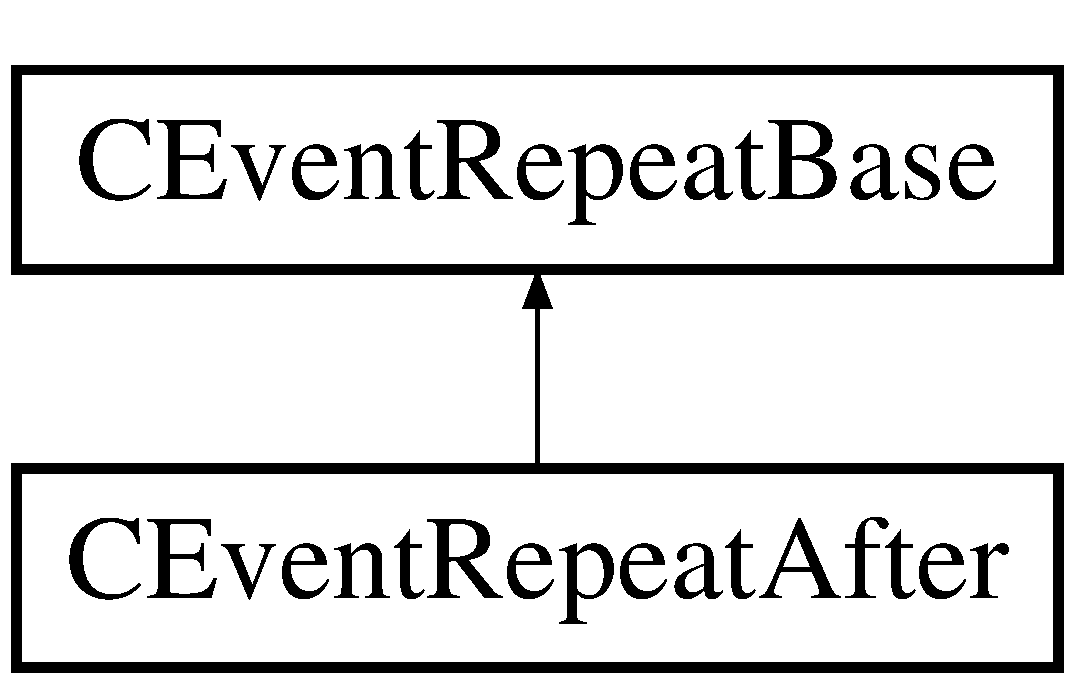
\includegraphics[height=2.000000cm]{class_c_event_repeat_after}
\end{center}
\end{figure}
\subsection*{Public Member Functions}
\begin{DoxyCompactItemize}
\item 
\mbox{\hyperlink{class_c_event_repeat_after_a6afc894472d7147d7dd57c27d9a5f12e}{C\+Event\+Repeat\+After}} (const \mbox{\hyperlink{class_c_duration}{C\+Duration}} \&duration)
\item 
\mbox{\hyperlink{class_c_event_repeat_base}{C\+Event\+Repeat\+Base}} $\ast$ \mbox{\hyperlink{class_c_event_repeat_after_ae635e551a44aeda7b155b7e5243a9872}{Clone}} () const override
\item 
\mbox{\hyperlink{class_c_event_repeat_after_a53a1a69bbeecb081673bfc4127bb8c01}{$\sim$\+C\+Event\+Repeat\+After}} () override=default
\item 
std\+::string \mbox{\hyperlink{class_c_event_repeat_after_a367f534544d07fde2ded54374152b9c3}{To\+Str}} () const override
\end{DoxyCompactItemize}
\subsection*{Protected Member Functions}
\begin{DoxyCompactItemize}
\item 
std\+::set$<$ \mbox{\hyperlink{class_c_date}{C\+Date}} $>$ \mbox{\hyperlink{class_c_event_repeat_after_ad4a4b0da551d754d657a10723b39d13c}{Test\+Range}} (const \mbox{\hyperlink{class_c_date}{C\+Date}} \&date, const \mbox{\hyperlink{class_c_date_af23472c977b14ed341b48183ec19d874}{C\+Date\+::\+Interval}} \&interval) const override
\end{DoxyCompactItemize}
\subsection*{Additional Inherited Members}


\subsection{Constructor \& Destructor Documentation}
\mbox{\Hypertarget{class_c_event_repeat_after_a6afc894472d7147d7dd57c27d9a5f12e}\label{class_c_event_repeat_after_a6afc894472d7147d7dd57c27d9a5f12e}} 
\index{C\+Event\+Repeat\+After@{C\+Event\+Repeat\+After}!C\+Event\+Repeat\+After@{C\+Event\+Repeat\+After}}
\index{C\+Event\+Repeat\+After@{C\+Event\+Repeat\+After}!C\+Event\+Repeat\+After@{C\+Event\+Repeat\+After}}
\subsubsection{\texorpdfstring{C\+Event\+Repeat\+After()}{CEventRepeatAfter()}}
{\footnotesize\ttfamily C\+Event\+Repeat\+After\+::\+C\+Event\+Repeat\+After (\begin{DoxyParamCaption}\item[{const \mbox{\hyperlink{class_c_duration}{C\+Duration}} \&}]{duration }\end{DoxyParamCaption})\hspace{0.3cm}{\ttfamily [inline]}, {\ttfamily [explicit]}}

\mbox{\Hypertarget{class_c_event_repeat_after_a53a1a69bbeecb081673bfc4127bb8c01}\label{class_c_event_repeat_after_a53a1a69bbeecb081673bfc4127bb8c01}} 
\index{C\+Event\+Repeat\+After@{C\+Event\+Repeat\+After}!````~C\+Event\+Repeat\+After@{$\sim$\+C\+Event\+Repeat\+After}}
\index{````~C\+Event\+Repeat\+After@{$\sim$\+C\+Event\+Repeat\+After}!C\+Event\+Repeat\+After@{C\+Event\+Repeat\+After}}
\subsubsection{\texorpdfstring{$\sim$\+C\+Event\+Repeat\+After()}{~CEventRepeatAfter()}}
{\footnotesize\ttfamily C\+Event\+Repeat\+After\+::$\sim$\+C\+Event\+Repeat\+After (\begin{DoxyParamCaption}{ }\end{DoxyParamCaption})\hspace{0.3cm}{\ttfamily [override]}, {\ttfamily [default]}}



\subsection{Member Function Documentation}
\mbox{\Hypertarget{class_c_event_repeat_after_ae635e551a44aeda7b155b7e5243a9872}\label{class_c_event_repeat_after_ae635e551a44aeda7b155b7e5243a9872}} 
\index{C\+Event\+Repeat\+After@{C\+Event\+Repeat\+After}!Clone@{Clone}}
\index{Clone@{Clone}!C\+Event\+Repeat\+After@{C\+Event\+Repeat\+After}}
\subsubsection{\texorpdfstring{Clone()}{Clone()}}
{\footnotesize\ttfamily \mbox{\hyperlink{class_c_event_repeat_base}{C\+Event\+Repeat\+Base}}$\ast$ C\+Event\+Repeat\+After\+::\+Clone (\begin{DoxyParamCaption}{ }\end{DoxyParamCaption}) const\hspace{0.3cm}{\ttfamily [inline]}, {\ttfamily [override]}, {\ttfamily [virtual]}}



Implements \mbox{\hyperlink{class_c_event_repeat_base_a73b079543ea6d97d38933b6a7544e349}{C\+Event\+Repeat\+Base}}.

\mbox{\Hypertarget{class_c_event_repeat_after_ad4a4b0da551d754d657a10723b39d13c}\label{class_c_event_repeat_after_ad4a4b0da551d754d657a10723b39d13c}} 
\index{C\+Event\+Repeat\+After@{C\+Event\+Repeat\+After}!Test\+Range@{Test\+Range}}
\index{Test\+Range@{Test\+Range}!C\+Event\+Repeat\+After@{C\+Event\+Repeat\+After}}
\subsubsection{\texorpdfstring{Test\+Range()}{TestRange()}}
{\footnotesize\ttfamily std\+::set$<$ \mbox{\hyperlink{class_c_date}{C\+Date}} $>$ C\+Event\+Repeat\+After\+::\+Test\+Range (\begin{DoxyParamCaption}\item[{const \mbox{\hyperlink{class_c_date}{C\+Date}} \&}]{date,  }\item[{const \mbox{\hyperlink{class_c_date_af23472c977b14ed341b48183ec19d874}{C\+Date\+::\+Interval}} \&}]{interval }\end{DoxyParamCaption}) const\hspace{0.3cm}{\ttfamily [override]}, {\ttfamily [protected]}, {\ttfamily [virtual]}}



Implements \mbox{\hyperlink{class_c_event_repeat_base_ad8371820b1c9771c93b452e4c80f4cea}{C\+Event\+Repeat\+Base}}.

\mbox{\Hypertarget{class_c_event_repeat_after_a367f534544d07fde2ded54374152b9c3}\label{class_c_event_repeat_after_a367f534544d07fde2ded54374152b9c3}} 
\index{C\+Event\+Repeat\+After@{C\+Event\+Repeat\+After}!To\+Str@{To\+Str}}
\index{To\+Str@{To\+Str}!C\+Event\+Repeat\+After@{C\+Event\+Repeat\+After}}
\subsubsection{\texorpdfstring{To\+Str()}{ToStr()}}
{\footnotesize\ttfamily std\+::string C\+Event\+Repeat\+After\+::\+To\+Str (\begin{DoxyParamCaption}{ }\end{DoxyParamCaption}) const\hspace{0.3cm}{\ttfamily [override]}, {\ttfamily [virtual]}}



Implements \mbox{\hyperlink{class_c_event_repeat_base_acf60d2b0890fdb3e701c944b26186197}{C\+Event\+Repeat\+Base}}.



The documentation for this class was generated from the following files\+:\begin{DoxyCompactItemize}
\item 
Repeat\+Strategies/\mbox{\hyperlink{_c_event_repeat_after_8h}{C\+Event\+Repeat\+After.\+h}}\item 
Repeat\+Strategies/\mbox{\hyperlink{_c_event_repeat_after_8cpp}{C\+Event\+Repeat\+After.\+cpp}}\end{DoxyCompactItemize}

\hypertarget{class_c_event_repeat_base}{}\section{C\+Event\+Repeat\+Base Class Reference}
\label{class_c_event_repeat_base}\index{C\+Event\+Repeat\+Base@{C\+Event\+Repeat\+Base}}


{\ttfamily \#include $<$C\+Event\+Repeat\+Base.\+h$>$}

Inheritance diagram for C\+Event\+Repeat\+Base\+:\begin{figure}[H]
\begin{center}
\leavevmode
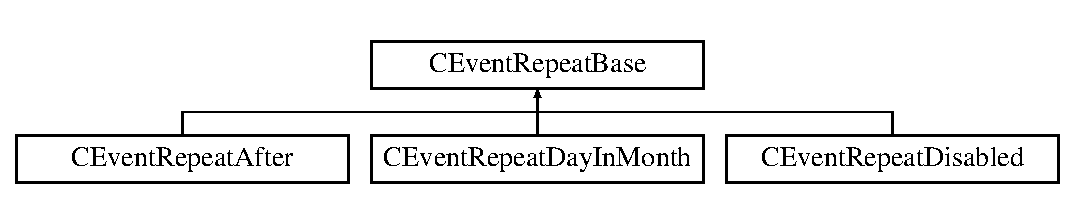
\includegraphics[height=2.000000cm]{class_c_event_repeat_base}
\end{center}
\end{figure}
\subsection*{Public Member Functions}
\begin{DoxyCompactItemize}
\item 
virtual \mbox{\hyperlink{class_c_event_repeat_base_a92978ac3d4425a8d70a0e491fffad471}{$\sim$\+C\+Event\+Repeat\+Base}} ()=default
\item 
virtual std\+::string \mbox{\hyperlink{class_c_event_repeat_base_acf60d2b0890fdb3e701c944b26186197}{To\+Str}} () const =0
\item 
virtual \mbox{\hyperlink{class_c_event_repeat_base}{C\+Event\+Repeat\+Base}} $\ast$ \mbox{\hyperlink{class_c_event_repeat_base_a73b079543ea6d97d38933b6a7544e349}{Clone}} () const =0
\item 
virtual std\+::set$<$ \mbox{\hyperlink{class_c_date}{C\+Date}} $>$ \mbox{\hyperlink{class_c_event_repeat_base_aac49d254d10deaed38bd83fad747f3b9}{Test\+Range\+With\+Exceptions}} (const \mbox{\hyperlink{class_c_date}{C\+Date}} \&date, const \mbox{\hyperlink{class_c_date_af23472c977b14ed341b48183ec19d874}{C\+Date\+::\+Interval}} \&interval)
\end{DoxyCompactItemize}
\subsection*{Static Public Member Functions}
\begin{DoxyCompactItemize}
\item 
static std\+::set$<$ std\+::pair$<$ \mbox{\hyperlink{class_c_date}{C\+Date}}, \mbox{\hyperlink{class_c_date}{C\+Date}} $>$ $>$ \mbox{\hyperlink{class_c_event_repeat_base_ab4f304478f81d70d9670e5e77e61de34}{Make\+Intervals}} (const std\+::set$<$ \mbox{\hyperlink{class_c_date}{C\+Date}} $>$ \&beginnings, const \mbox{\hyperlink{class_c_duration}{C\+Duration}} \&duration)
\end{DoxyCompactItemize}
\subsection*{Public Attributes}
\begin{DoxyCompactItemize}
\item 
std\+::set$<$ \mbox{\hyperlink{class_c_date}{C\+Date}} $>$ \mbox{\hyperlink{class_c_event_repeat_base_a8080eddd346a489c9a04573761895d53}{m\+\_\+\+Additional}}
\item 
std\+::set$<$ \mbox{\hyperlink{class_c_date}{C\+Date}} $>$ \mbox{\hyperlink{class_c_event_repeat_base_a754e059274866f1338e68307894b1602}{m\+\_\+\+Skipped}}
\end{DoxyCompactItemize}
\subsection*{Protected Member Functions}
\begin{DoxyCompactItemize}
\item 
virtual std\+::set$<$ \mbox{\hyperlink{class_c_date}{C\+Date}} $>$ \mbox{\hyperlink{class_c_event_repeat_base_ad8371820b1c9771c93b452e4c80f4cea}{Test\+Range}} (const \mbox{\hyperlink{class_c_date}{C\+Date}} \&date, const \mbox{\hyperlink{class_c_date_af23472c977b14ed341b48183ec19d874}{C\+Date\+::\+Interval}} \&interval) const =0
\end{DoxyCompactItemize}


\subsection{Constructor \& Destructor Documentation}
\mbox{\Hypertarget{class_c_event_repeat_base_a92978ac3d4425a8d70a0e491fffad471}\label{class_c_event_repeat_base_a92978ac3d4425a8d70a0e491fffad471}} 
\index{C\+Event\+Repeat\+Base@{C\+Event\+Repeat\+Base}!````~C\+Event\+Repeat\+Base@{$\sim$\+C\+Event\+Repeat\+Base}}
\index{````~C\+Event\+Repeat\+Base@{$\sim$\+C\+Event\+Repeat\+Base}!C\+Event\+Repeat\+Base@{C\+Event\+Repeat\+Base}}
\subsubsection{\texorpdfstring{$\sim$\+C\+Event\+Repeat\+Base()}{~CEventRepeatBase()}}
{\footnotesize\ttfamily virtual C\+Event\+Repeat\+Base\+::$\sim$\+C\+Event\+Repeat\+Base (\begin{DoxyParamCaption}{ }\end{DoxyParamCaption})\hspace{0.3cm}{\ttfamily [virtual]}, {\ttfamily [default]}}



\subsection{Member Function Documentation}
\mbox{\Hypertarget{class_c_event_repeat_base_a73b079543ea6d97d38933b6a7544e349}\label{class_c_event_repeat_base_a73b079543ea6d97d38933b6a7544e349}} 
\index{C\+Event\+Repeat\+Base@{C\+Event\+Repeat\+Base}!Clone@{Clone}}
\index{Clone@{Clone}!C\+Event\+Repeat\+Base@{C\+Event\+Repeat\+Base}}
\subsubsection{\texorpdfstring{Clone()}{Clone()}}
{\footnotesize\ttfamily virtual \mbox{\hyperlink{class_c_event_repeat_base}{C\+Event\+Repeat\+Base}}$\ast$ C\+Event\+Repeat\+Base\+::\+Clone (\begin{DoxyParamCaption}{ }\end{DoxyParamCaption}) const\hspace{0.3cm}{\ttfamily [pure virtual]}}



Implemented in \mbox{\hyperlink{class_c_event_repeat_day_in_month_a329373945107435d629ecc2491ce8b38}{C\+Event\+Repeat\+Day\+In\+Month}}, \mbox{\hyperlink{class_c_event_repeat_after_ae635e551a44aeda7b155b7e5243a9872}{C\+Event\+Repeat\+After}}, and \mbox{\hyperlink{class_c_event_repeat_disabled_afc00861b70904d48410ea17db3555da1}{C\+Event\+Repeat\+Disabled}}.

\mbox{\Hypertarget{class_c_event_repeat_base_ab4f304478f81d70d9670e5e77e61de34}\label{class_c_event_repeat_base_ab4f304478f81d70d9670e5e77e61de34}} 
\index{C\+Event\+Repeat\+Base@{C\+Event\+Repeat\+Base}!Make\+Intervals@{Make\+Intervals}}
\index{Make\+Intervals@{Make\+Intervals}!C\+Event\+Repeat\+Base@{C\+Event\+Repeat\+Base}}
\subsubsection{\texorpdfstring{Make\+Intervals()}{MakeIntervals()}}
{\footnotesize\ttfamily std\+::set$<$ \mbox{\hyperlink{class_c_date_af23472c977b14ed341b48183ec19d874}{C\+Date\+::\+Interval}} $>$ C\+Event\+Repeat\+Base\+::\+Make\+Intervals (\begin{DoxyParamCaption}\item[{const std\+::set$<$ \mbox{\hyperlink{class_c_date}{C\+Date}} $>$ \&}]{beginnings,  }\item[{const \mbox{\hyperlink{class_c_duration}{C\+Duration}} \&}]{duration }\end{DoxyParamCaption})\hspace{0.3cm}{\ttfamily [static]}}

\mbox{\Hypertarget{class_c_event_repeat_base_ad8371820b1c9771c93b452e4c80f4cea}\label{class_c_event_repeat_base_ad8371820b1c9771c93b452e4c80f4cea}} 
\index{C\+Event\+Repeat\+Base@{C\+Event\+Repeat\+Base}!Test\+Range@{Test\+Range}}
\index{Test\+Range@{Test\+Range}!C\+Event\+Repeat\+Base@{C\+Event\+Repeat\+Base}}
\subsubsection{\texorpdfstring{Test\+Range()}{TestRange()}}
{\footnotesize\ttfamily virtual std\+::set$<$\mbox{\hyperlink{class_c_date}{C\+Date}}$>$ C\+Event\+Repeat\+Base\+::\+Test\+Range (\begin{DoxyParamCaption}\item[{const \mbox{\hyperlink{class_c_date}{C\+Date}} \&}]{date,  }\item[{const \mbox{\hyperlink{class_c_date_af23472c977b14ed341b48183ec19d874}{C\+Date\+::\+Interval}} \&}]{interval }\end{DoxyParamCaption}) const\hspace{0.3cm}{\ttfamily [protected]}, {\ttfamily [pure virtual]}}



Implemented in \mbox{\hyperlink{class_c_event_repeat_day_in_month_a84de2696efb387af591bff04f37fd7ed}{C\+Event\+Repeat\+Day\+In\+Month}}, \mbox{\hyperlink{class_c_event_repeat_disabled_a0d9196c321d405660223d46c3c1ab27e}{C\+Event\+Repeat\+Disabled}}, and \mbox{\hyperlink{class_c_event_repeat_after_ad4a4b0da551d754d657a10723b39d13c}{C\+Event\+Repeat\+After}}.

\mbox{\Hypertarget{class_c_event_repeat_base_aac49d254d10deaed38bd83fad747f3b9}\label{class_c_event_repeat_base_aac49d254d10deaed38bd83fad747f3b9}} 
\index{C\+Event\+Repeat\+Base@{C\+Event\+Repeat\+Base}!Test\+Range\+With\+Exceptions@{Test\+Range\+With\+Exceptions}}
\index{Test\+Range\+With\+Exceptions@{Test\+Range\+With\+Exceptions}!C\+Event\+Repeat\+Base@{C\+Event\+Repeat\+Base}}
\subsubsection{\texorpdfstring{Test\+Range\+With\+Exceptions()}{TestRangeWithExceptions()}}
{\footnotesize\ttfamily std\+::set$<$ \mbox{\hyperlink{class_c_date}{C\+Date}} $>$ C\+Event\+Repeat\+Base\+::\+Test\+Range\+With\+Exceptions (\begin{DoxyParamCaption}\item[{const \mbox{\hyperlink{class_c_date}{C\+Date}} \&}]{date,  }\item[{const \mbox{\hyperlink{class_c_date_af23472c977b14ed341b48183ec19d874}{C\+Date\+::\+Interval}} \&}]{interval }\end{DoxyParamCaption})\hspace{0.3cm}{\ttfamily [virtual]}}

\mbox{\Hypertarget{class_c_event_repeat_base_acf60d2b0890fdb3e701c944b26186197}\label{class_c_event_repeat_base_acf60d2b0890fdb3e701c944b26186197}} 
\index{C\+Event\+Repeat\+Base@{C\+Event\+Repeat\+Base}!To\+Str@{To\+Str}}
\index{To\+Str@{To\+Str}!C\+Event\+Repeat\+Base@{C\+Event\+Repeat\+Base}}
\subsubsection{\texorpdfstring{To\+Str()}{ToStr()}}
{\footnotesize\ttfamily virtual std\+::string C\+Event\+Repeat\+Base\+::\+To\+Str (\begin{DoxyParamCaption}{ }\end{DoxyParamCaption}) const\hspace{0.3cm}{\ttfamily [pure virtual]}}



Implemented in \mbox{\hyperlink{class_c_event_repeat_day_in_month_a5ec4554d0d7c1c9a50cd1f37f0d76673}{C\+Event\+Repeat\+Day\+In\+Month}}, \mbox{\hyperlink{class_c_event_repeat_after_a367f534544d07fde2ded54374152b9c3}{C\+Event\+Repeat\+After}}, and \mbox{\hyperlink{class_c_event_repeat_disabled_a58cfa9f6921c351c85f747e80183842b}{C\+Event\+Repeat\+Disabled}}.



\subsection{Member Data Documentation}
\mbox{\Hypertarget{class_c_event_repeat_base_a8080eddd346a489c9a04573761895d53}\label{class_c_event_repeat_base_a8080eddd346a489c9a04573761895d53}} 
\index{C\+Event\+Repeat\+Base@{C\+Event\+Repeat\+Base}!m\+\_\+\+Additional@{m\+\_\+\+Additional}}
\index{m\+\_\+\+Additional@{m\+\_\+\+Additional}!C\+Event\+Repeat\+Base@{C\+Event\+Repeat\+Base}}
\subsubsection{\texorpdfstring{m\+\_\+\+Additional}{m\_Additional}}
{\footnotesize\ttfamily std\+::set$<$\mbox{\hyperlink{class_c_date}{C\+Date}}$>$ C\+Event\+Repeat\+Base\+::m\+\_\+\+Additional}

\mbox{\Hypertarget{class_c_event_repeat_base_a754e059274866f1338e68307894b1602}\label{class_c_event_repeat_base_a754e059274866f1338e68307894b1602}} 
\index{C\+Event\+Repeat\+Base@{C\+Event\+Repeat\+Base}!m\+\_\+\+Skipped@{m\+\_\+\+Skipped}}
\index{m\+\_\+\+Skipped@{m\+\_\+\+Skipped}!C\+Event\+Repeat\+Base@{C\+Event\+Repeat\+Base}}
\subsubsection{\texorpdfstring{m\+\_\+\+Skipped}{m\_Skipped}}
{\footnotesize\ttfamily std\+::set$<$\mbox{\hyperlink{class_c_date}{C\+Date}}$>$ C\+Event\+Repeat\+Base\+::m\+\_\+\+Skipped}



The documentation for this class was generated from the following files\+:\begin{DoxyCompactItemize}
\item 
Repeat\+Strategies/\mbox{\hyperlink{_c_event_repeat_base_8h}{C\+Event\+Repeat\+Base.\+h}}\item 
Repeat\+Strategies/\mbox{\hyperlink{_c_event_repeat_base_8cpp}{C\+Event\+Repeat\+Base.\+cpp}}\end{DoxyCompactItemize}

\hypertarget{class_c_event_repeat_day_in_month}{}\section{C\+Event\+Repeat\+Day\+In\+Month Class Reference}
\label{class_c_event_repeat_day_in_month}\index{C\+Event\+Repeat\+Day\+In\+Month@{C\+Event\+Repeat\+Day\+In\+Month}}


{\ttfamily \#include $<$C\+Event\+Repeat\+Day\+In\+Month.\+h$>$}

Inheritance diagram for C\+Event\+Repeat\+Day\+In\+Month\+:\begin{figure}[H]
\begin{center}
\leavevmode
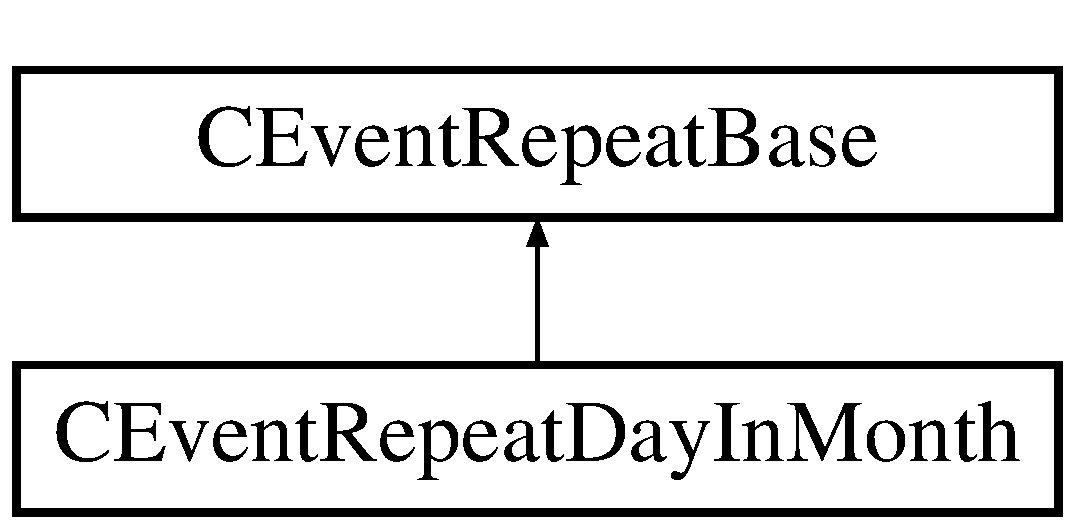
\includegraphics[height=2.000000cm]{class_c_event_repeat_day_in_month}
\end{center}
\end{figure}
\subsection*{Public Member Functions}
\begin{DoxyCompactItemize}
\item 
\mbox{\hyperlink{class_c_event_repeat_day_in_month_a161460e3eeb9fa2a027d39004828a760}{C\+Event\+Repeat\+Day\+In\+Month}} (int day)
\item 
\mbox{\hyperlink{class_c_event_repeat_day_in_month_a37483901cea40744356c63cc491f759a}{$\sim$\+C\+Event\+Repeat\+Day\+In\+Month}} () override=default
\item 
\mbox{\hyperlink{class_c_event_repeat_base}{C\+Event\+Repeat\+Base}} $\ast$ \mbox{\hyperlink{class_c_event_repeat_day_in_month_a329373945107435d629ecc2491ce8b38}{Clone}} () const override
\item 
std\+::string \mbox{\hyperlink{class_c_event_repeat_day_in_month_a5ec4554d0d7c1c9a50cd1f37f0d76673}{To\+Str}} () const override
\end{DoxyCompactItemize}
\subsection*{Protected Member Functions}
\begin{DoxyCompactItemize}
\item 
std\+::set$<$ \mbox{\hyperlink{class_c_date}{C\+Date}} $>$ \mbox{\hyperlink{class_c_event_repeat_day_in_month_a84de2696efb387af591bff04f37fd7ed}{Test\+Range}} (const \mbox{\hyperlink{class_c_date}{C\+Date}} \&date, const \mbox{\hyperlink{class_c_date_af23472c977b14ed341b48183ec19d874}{C\+Date\+::\+Interval}} \&interval) const override
\end{DoxyCompactItemize}
\subsection*{Additional Inherited Members}


\subsection{Detailed Description}
Allows expressions like 10. day in month. Or last day of month. 

\subsection{Constructor \& Destructor Documentation}
\mbox{\Hypertarget{class_c_event_repeat_day_in_month_a161460e3eeb9fa2a027d39004828a760}\label{class_c_event_repeat_day_in_month_a161460e3eeb9fa2a027d39004828a760}} 
\index{C\+Event\+Repeat\+Day\+In\+Month@{C\+Event\+Repeat\+Day\+In\+Month}!C\+Event\+Repeat\+Day\+In\+Month@{C\+Event\+Repeat\+Day\+In\+Month}}
\index{C\+Event\+Repeat\+Day\+In\+Month@{C\+Event\+Repeat\+Day\+In\+Month}!C\+Event\+Repeat\+Day\+In\+Month@{C\+Event\+Repeat\+Day\+In\+Month}}
\subsubsection{\texorpdfstring{C\+Event\+Repeat\+Day\+In\+Month()}{CEventRepeatDayInMonth()}}
{\footnotesize\ttfamily C\+Event\+Repeat\+Day\+In\+Month\+::\+C\+Event\+Repeat\+Day\+In\+Month (\begin{DoxyParamCaption}\item[{int}]{day }\end{DoxyParamCaption})\hspace{0.3cm}{\ttfamily [inline]}, {\ttfamily [explicit]}}

Constructor 
\begin{DoxyParams}{Parameters}
{\em day} & Non-\/zero number between -\/31 and 31. Negative value means from the back. E. g. -\/1 in January means 31. In February 28 and 29 for non-\/leap and leap respectively. Throws invalid\+\_\+argument if out of boundaries. Event will not trigger if day is 30 and month is February. \\
\hline
\end{DoxyParams}
\mbox{\Hypertarget{class_c_event_repeat_day_in_month_a37483901cea40744356c63cc491f759a}\label{class_c_event_repeat_day_in_month_a37483901cea40744356c63cc491f759a}} 
\index{C\+Event\+Repeat\+Day\+In\+Month@{C\+Event\+Repeat\+Day\+In\+Month}!````~C\+Event\+Repeat\+Day\+In\+Month@{$\sim$\+C\+Event\+Repeat\+Day\+In\+Month}}
\index{````~C\+Event\+Repeat\+Day\+In\+Month@{$\sim$\+C\+Event\+Repeat\+Day\+In\+Month}!C\+Event\+Repeat\+Day\+In\+Month@{C\+Event\+Repeat\+Day\+In\+Month}}
\subsubsection{\texorpdfstring{$\sim$\+C\+Event\+Repeat\+Day\+In\+Month()}{~CEventRepeatDayInMonth()}}
{\footnotesize\ttfamily C\+Event\+Repeat\+Day\+In\+Month\+::$\sim$\+C\+Event\+Repeat\+Day\+In\+Month (\begin{DoxyParamCaption}{ }\end{DoxyParamCaption})\hspace{0.3cm}{\ttfamily [override]}, {\ttfamily [default]}}



\subsection{Member Function Documentation}
\mbox{\Hypertarget{class_c_event_repeat_day_in_month_a329373945107435d629ecc2491ce8b38}\label{class_c_event_repeat_day_in_month_a329373945107435d629ecc2491ce8b38}} 
\index{C\+Event\+Repeat\+Day\+In\+Month@{C\+Event\+Repeat\+Day\+In\+Month}!Clone@{Clone}}
\index{Clone@{Clone}!C\+Event\+Repeat\+Day\+In\+Month@{C\+Event\+Repeat\+Day\+In\+Month}}
\subsubsection{\texorpdfstring{Clone()}{Clone()}}
{\footnotesize\ttfamily \mbox{\hyperlink{class_c_event_repeat_base}{C\+Event\+Repeat\+Base}}$\ast$ C\+Event\+Repeat\+Day\+In\+Month\+::\+Clone (\begin{DoxyParamCaption}{ }\end{DoxyParamCaption}) const\hspace{0.3cm}{\ttfamily [inline]}, {\ttfamily [override]}, {\ttfamily [virtual]}}



Implements \mbox{\hyperlink{class_c_event_repeat_base_a73b079543ea6d97d38933b6a7544e349}{C\+Event\+Repeat\+Base}}.

\mbox{\Hypertarget{class_c_event_repeat_day_in_month_a84de2696efb387af591bff04f37fd7ed}\label{class_c_event_repeat_day_in_month_a84de2696efb387af591bff04f37fd7ed}} 
\index{C\+Event\+Repeat\+Day\+In\+Month@{C\+Event\+Repeat\+Day\+In\+Month}!Test\+Range@{Test\+Range}}
\index{Test\+Range@{Test\+Range}!C\+Event\+Repeat\+Day\+In\+Month@{C\+Event\+Repeat\+Day\+In\+Month}}
\subsubsection{\texorpdfstring{Test\+Range()}{TestRange()}}
{\footnotesize\ttfamily std\+::set$<$ \mbox{\hyperlink{class_c_date}{C\+Date}} $>$ C\+Event\+Repeat\+Day\+In\+Month\+::\+Test\+Range (\begin{DoxyParamCaption}\item[{const \mbox{\hyperlink{class_c_date}{C\+Date}} \&}]{date,  }\item[{const \mbox{\hyperlink{class_c_date_af23472c977b14ed341b48183ec19d874}{C\+Date\+::\+Interval}} \&}]{interval }\end{DoxyParamCaption}) const\hspace{0.3cm}{\ttfamily [override]}, {\ttfamily [protected]}, {\ttfamily [virtual]}}



Implements \mbox{\hyperlink{class_c_event_repeat_base_ad8371820b1c9771c93b452e4c80f4cea}{C\+Event\+Repeat\+Base}}.

\mbox{\Hypertarget{class_c_event_repeat_day_in_month_a5ec4554d0d7c1c9a50cd1f37f0d76673}\label{class_c_event_repeat_day_in_month_a5ec4554d0d7c1c9a50cd1f37f0d76673}} 
\index{C\+Event\+Repeat\+Day\+In\+Month@{C\+Event\+Repeat\+Day\+In\+Month}!To\+Str@{To\+Str}}
\index{To\+Str@{To\+Str}!C\+Event\+Repeat\+Day\+In\+Month@{C\+Event\+Repeat\+Day\+In\+Month}}
\subsubsection{\texorpdfstring{To\+Str()}{ToStr()}}
{\footnotesize\ttfamily std\+::string C\+Event\+Repeat\+Day\+In\+Month\+::\+To\+Str (\begin{DoxyParamCaption}{ }\end{DoxyParamCaption}) const\hspace{0.3cm}{\ttfamily [override]}, {\ttfamily [virtual]}}



Implements \mbox{\hyperlink{class_c_event_repeat_base_acf60d2b0890fdb3e701c944b26186197}{C\+Event\+Repeat\+Base}}.



The documentation for this class was generated from the following files\+:\begin{DoxyCompactItemize}
\item 
Repeat\+Strategies/\mbox{\hyperlink{_c_event_repeat_day_in_month_8h}{C\+Event\+Repeat\+Day\+In\+Month.\+h}}\item 
Repeat\+Strategies/\mbox{\hyperlink{_c_event_repeat_day_in_month_8cpp}{C\+Event\+Repeat\+Day\+In\+Month.\+cpp}}\end{DoxyCompactItemize}

\hypertarget{class_c_event_repeat_disabled}{}\section{C\+Event\+Repeat\+Disabled Class Reference}
\label{class_c_event_repeat_disabled}\index{C\+Event\+Repeat\+Disabled@{C\+Event\+Repeat\+Disabled}}


{\ttfamily \#include $<$C\+Event\+Repeat\+Disabled.\+h$>$}

Inheritance diagram for C\+Event\+Repeat\+Disabled\+:\begin{figure}[H]
\begin{center}
\leavevmode
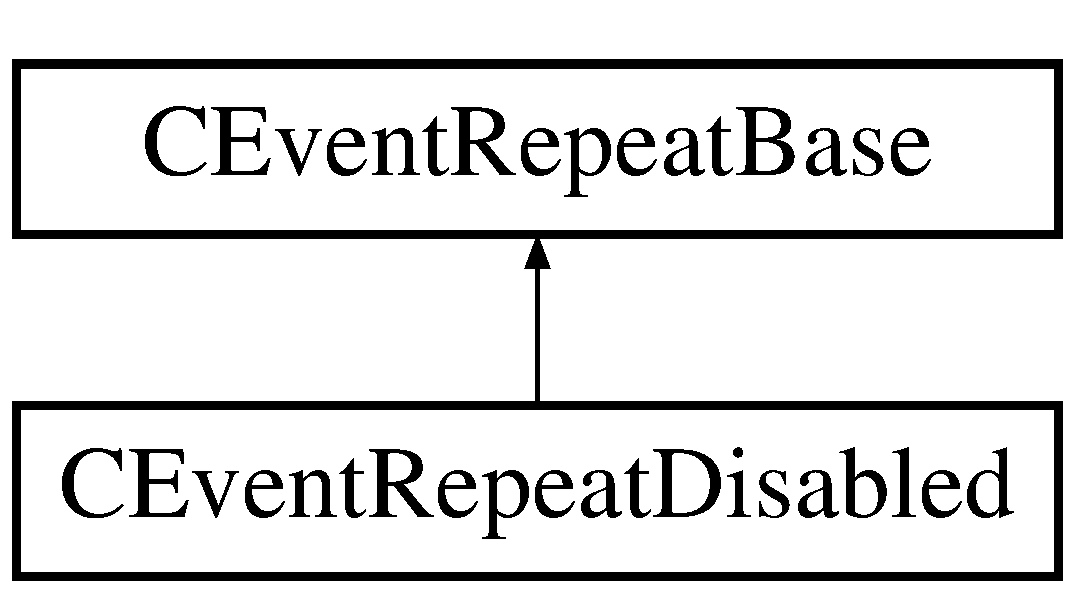
\includegraphics[height=2.000000cm]{class_c_event_repeat_disabled}
\end{center}
\end{figure}
\subsection*{Public Member Functions}
\begin{DoxyCompactItemize}
\item 
\mbox{\hyperlink{class_c_event_repeat_disabled_a3ab08c68323db33b823f3232b02dd5ac}{$\sim$\+C\+Event\+Repeat\+Disabled}} () override=default
\item 
\mbox{\hyperlink{class_c_event_repeat_base}{C\+Event\+Repeat\+Base}} $\ast$ \mbox{\hyperlink{class_c_event_repeat_disabled_afc00861b70904d48410ea17db3555da1}{Clone}} () const override
\item 
std\+::string \mbox{\hyperlink{class_c_event_repeat_disabled_a58cfa9f6921c351c85f747e80183842b}{To\+Str}} () const override
\end{DoxyCompactItemize}
\subsection*{Protected Member Functions}
\begin{DoxyCompactItemize}
\item 
std\+::set$<$ \mbox{\hyperlink{class_c_date}{C\+Date}} $>$ \mbox{\hyperlink{class_c_event_repeat_disabled_a0d9196c321d405660223d46c3c1ab27e}{Test\+Range}} (const \mbox{\hyperlink{class_c_date}{C\+Date}} \&date, const \mbox{\hyperlink{class_c_date_af23472c977b14ed341b48183ec19d874}{C\+Date\+::\+Interval}} \&interval) const override
\end{DoxyCompactItemize}
\subsection*{Additional Inherited Members}


\subsection{Constructor \& Destructor Documentation}
\mbox{\Hypertarget{class_c_event_repeat_disabled_a3ab08c68323db33b823f3232b02dd5ac}\label{class_c_event_repeat_disabled_a3ab08c68323db33b823f3232b02dd5ac}} 
\index{C\+Event\+Repeat\+Disabled@{C\+Event\+Repeat\+Disabled}!````~C\+Event\+Repeat\+Disabled@{$\sim$\+C\+Event\+Repeat\+Disabled}}
\index{````~C\+Event\+Repeat\+Disabled@{$\sim$\+C\+Event\+Repeat\+Disabled}!C\+Event\+Repeat\+Disabled@{C\+Event\+Repeat\+Disabled}}
\subsubsection{\texorpdfstring{$\sim$\+C\+Event\+Repeat\+Disabled()}{~CEventRepeatDisabled()}}
{\footnotesize\ttfamily C\+Event\+Repeat\+Disabled\+::$\sim$\+C\+Event\+Repeat\+Disabled (\begin{DoxyParamCaption}{ }\end{DoxyParamCaption})\hspace{0.3cm}{\ttfamily [override]}, {\ttfamily [default]}}



\subsection{Member Function Documentation}
\mbox{\Hypertarget{class_c_event_repeat_disabled_afc00861b70904d48410ea17db3555da1}\label{class_c_event_repeat_disabled_afc00861b70904d48410ea17db3555da1}} 
\index{C\+Event\+Repeat\+Disabled@{C\+Event\+Repeat\+Disabled}!Clone@{Clone}}
\index{Clone@{Clone}!C\+Event\+Repeat\+Disabled@{C\+Event\+Repeat\+Disabled}}
\subsubsection{\texorpdfstring{Clone()}{Clone()}}
{\footnotesize\ttfamily \mbox{\hyperlink{class_c_event_repeat_base}{C\+Event\+Repeat\+Base}}$\ast$ C\+Event\+Repeat\+Disabled\+::\+Clone (\begin{DoxyParamCaption}{ }\end{DoxyParamCaption}) const\hspace{0.3cm}{\ttfamily [inline]}, {\ttfamily [override]}, {\ttfamily [virtual]}}



Implements \mbox{\hyperlink{class_c_event_repeat_base_a73b079543ea6d97d38933b6a7544e349}{C\+Event\+Repeat\+Base}}.

\mbox{\Hypertarget{class_c_event_repeat_disabled_a0d9196c321d405660223d46c3c1ab27e}\label{class_c_event_repeat_disabled_a0d9196c321d405660223d46c3c1ab27e}} 
\index{C\+Event\+Repeat\+Disabled@{C\+Event\+Repeat\+Disabled}!Test\+Range@{Test\+Range}}
\index{Test\+Range@{Test\+Range}!C\+Event\+Repeat\+Disabled@{C\+Event\+Repeat\+Disabled}}
\subsubsection{\texorpdfstring{Test\+Range()}{TestRange()}}
{\footnotesize\ttfamily std\+::set$<$ \mbox{\hyperlink{class_c_date}{C\+Date}} $>$ C\+Event\+Repeat\+Disabled\+::\+Test\+Range (\begin{DoxyParamCaption}\item[{const \mbox{\hyperlink{class_c_date}{C\+Date}} \&}]{date,  }\item[{const \mbox{\hyperlink{class_c_date_af23472c977b14ed341b48183ec19d874}{C\+Date\+::\+Interval}} \&}]{interval }\end{DoxyParamCaption}) const\hspace{0.3cm}{\ttfamily [override]}, {\ttfamily [protected]}, {\ttfamily [virtual]}}



Implements \mbox{\hyperlink{class_c_event_repeat_base_ad8371820b1c9771c93b452e4c80f4cea}{C\+Event\+Repeat\+Base}}.

\mbox{\Hypertarget{class_c_event_repeat_disabled_a58cfa9f6921c351c85f747e80183842b}\label{class_c_event_repeat_disabled_a58cfa9f6921c351c85f747e80183842b}} 
\index{C\+Event\+Repeat\+Disabled@{C\+Event\+Repeat\+Disabled}!To\+Str@{To\+Str}}
\index{To\+Str@{To\+Str}!C\+Event\+Repeat\+Disabled@{C\+Event\+Repeat\+Disabled}}
\subsubsection{\texorpdfstring{To\+Str()}{ToStr()}}
{\footnotesize\ttfamily std\+::string C\+Event\+Repeat\+Disabled\+::\+To\+Str (\begin{DoxyParamCaption}{ }\end{DoxyParamCaption}) const\hspace{0.3cm}{\ttfamily [override]}, {\ttfamily [virtual]}}



Implements \mbox{\hyperlink{class_c_event_repeat_base_acf60d2b0890fdb3e701c944b26186197}{C\+Event\+Repeat\+Base}}.



The documentation for this class was generated from the following files\+:\begin{DoxyCompactItemize}
\item 
Repeat\+Strategies/\mbox{\hyperlink{_c_event_repeat_disabled_8h}{C\+Event\+Repeat\+Disabled.\+h}}\item 
Repeat\+Strategies/\mbox{\hyperlink{_c_event_repeat_disabled_8cpp}{C\+Event\+Repeat\+Disabled.\+cpp}}\end{DoxyCompactItemize}

\hypertarget{class_c_event_transfer_base}{}\section{C\+Event\+Transfer\+Base Class Reference}
\label{class_c_event_transfer_base}\index{C\+Event\+Transfer\+Base@{C\+Event\+Transfer\+Base}}


{\ttfamily \#include $<$C\+Event\+Transfer\+Base.\+h$>$}

Inheritance diagram for C\+Event\+Transfer\+Base\+:\begin{figure}[H]
\begin{center}
\leavevmode
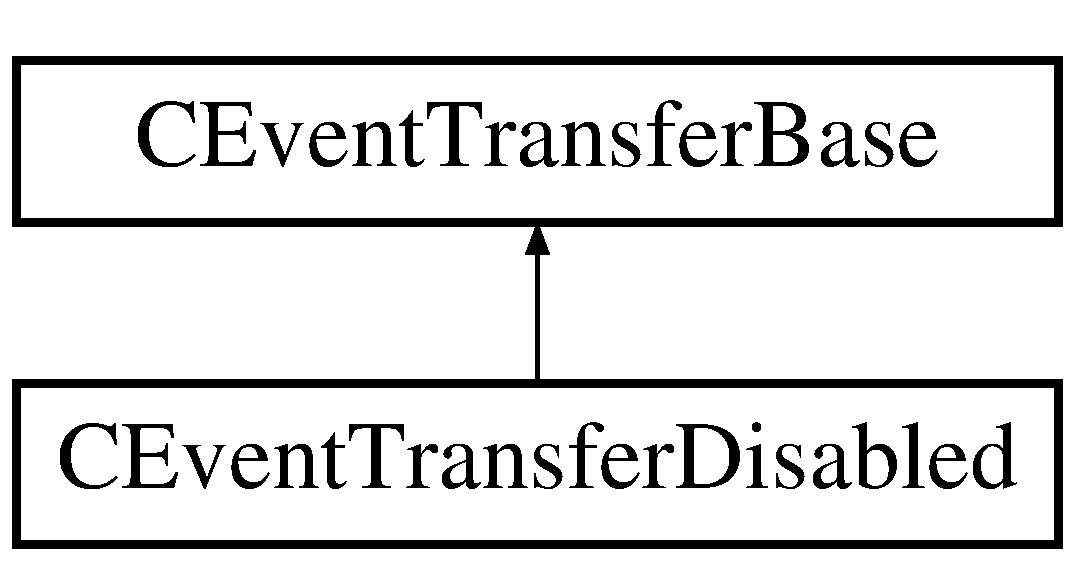
\includegraphics[height=2.000000cm]{class_c_event_transfer_base}
\end{center}
\end{figure}
\subsection*{Public Member Functions}
\begin{DoxyCompactItemize}
\item 
virtual \mbox{\hyperlink{class_c_event_transfer_base_a94196ebb46e7ae58fa72d83a790ebaaf}{$\sim$\+C\+Event\+Transfer\+Base}} ()=default
\item 
virtual bool \mbox{\hyperlink{class_c_event_transfer_base_aa72518d8ee05349865216c8e60459669}{Transfer\+Possible}} (const \mbox{\hyperlink{class_c_date}{C\+Date}} \&from, const \mbox{\hyperlink{class_c_date}{C\+Date}} \&to) const =0
\end{DoxyCompactItemize}


\subsection{Constructor \& Destructor Documentation}
\mbox{\Hypertarget{class_c_event_transfer_base_a94196ebb46e7ae58fa72d83a790ebaaf}\label{class_c_event_transfer_base_a94196ebb46e7ae58fa72d83a790ebaaf}} 
\index{C\+Event\+Transfer\+Base@{C\+Event\+Transfer\+Base}!````~C\+Event\+Transfer\+Base@{$\sim$\+C\+Event\+Transfer\+Base}}
\index{````~C\+Event\+Transfer\+Base@{$\sim$\+C\+Event\+Transfer\+Base}!C\+Event\+Transfer\+Base@{C\+Event\+Transfer\+Base}}
\subsubsection{\texorpdfstring{$\sim$\+C\+Event\+Transfer\+Base()}{~CEventTransferBase()}}
{\footnotesize\ttfamily virtual C\+Event\+Transfer\+Base\+::$\sim$\+C\+Event\+Transfer\+Base (\begin{DoxyParamCaption}{ }\end{DoxyParamCaption})\hspace{0.3cm}{\ttfamily [virtual]}, {\ttfamily [default]}}



\subsection{Member Function Documentation}
\mbox{\Hypertarget{class_c_event_transfer_base_aa72518d8ee05349865216c8e60459669}\label{class_c_event_transfer_base_aa72518d8ee05349865216c8e60459669}} 
\index{C\+Event\+Transfer\+Base@{C\+Event\+Transfer\+Base}!Transfer\+Possible@{Transfer\+Possible}}
\index{Transfer\+Possible@{Transfer\+Possible}!C\+Event\+Transfer\+Base@{C\+Event\+Transfer\+Base}}
\subsubsection{\texorpdfstring{Transfer\+Possible()}{TransferPossible()}}
{\footnotesize\ttfamily virtual bool C\+Event\+Transfer\+Base\+::\+Transfer\+Possible (\begin{DoxyParamCaption}\item[{const \mbox{\hyperlink{class_c_date}{C\+Date}} \&}]{from,  }\item[{const \mbox{\hyperlink{class_c_date}{C\+Date}} \&}]{to }\end{DoxyParamCaption}) const\hspace{0.3cm}{\ttfamily [pure virtual]}}



Implemented in \mbox{\hyperlink{class_c_event_transfer_disabled_a5015ce168c3fcba4a20381256f901c3a}{C\+Event\+Transfer\+Disabled}}.



The documentation for this class was generated from the following file\+:\begin{DoxyCompactItemize}
\item 
Transfer\+Strategies/\mbox{\hyperlink{_c_event_transfer_base_8h}{C\+Event\+Transfer\+Base.\+h}}\end{DoxyCompactItemize}

\hypertarget{class_c_event_transfer_disabled}{}\section{C\+Event\+Transfer\+Disabled Class Reference}
\label{class_c_event_transfer_disabled}\index{C\+Event\+Transfer\+Disabled@{C\+Event\+Transfer\+Disabled}}


{\ttfamily \#include $<$C\+Event\+Transfer\+Disabled.\+h$>$}

Inheritance diagram for C\+Event\+Transfer\+Disabled\+:\begin{figure}[H]
\begin{center}
\leavevmode
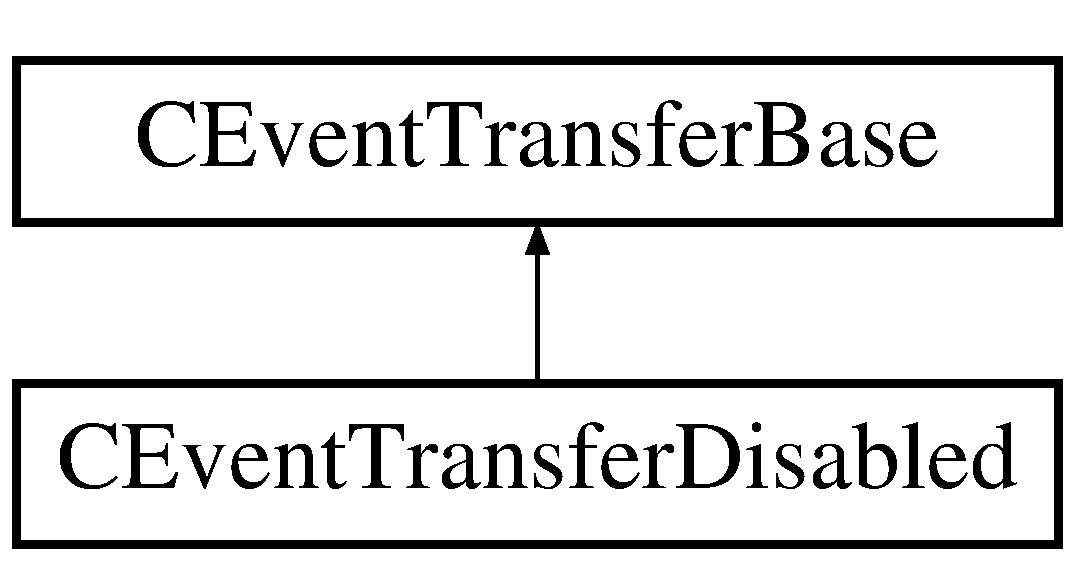
\includegraphics[height=2.000000cm]{class_c_event_transfer_disabled}
\end{center}
\end{figure}
\subsection*{Public Member Functions}
\begin{DoxyCompactItemize}
\item 
\mbox{\hyperlink{class_c_event_transfer_disabled_a3daa2c2c89449d98faeab6a57e57b8e7}{$\sim$\+C\+Event\+Transfer\+Disabled}} () override
\item 
bool \mbox{\hyperlink{class_c_event_transfer_disabled_a5015ce168c3fcba4a20381256f901c3a}{Transfer\+Possible}} (const \mbox{\hyperlink{class_c_date}{C\+Date}} \&from, const \mbox{\hyperlink{class_c_date}{C\+Date}} \&to) const override
\end{DoxyCompactItemize}


\subsection{Constructor \& Destructor Documentation}
\mbox{\Hypertarget{class_c_event_transfer_disabled_a3daa2c2c89449d98faeab6a57e57b8e7}\label{class_c_event_transfer_disabled_a3daa2c2c89449d98faeab6a57e57b8e7}} 
\index{C\+Event\+Transfer\+Disabled@{C\+Event\+Transfer\+Disabled}!````~C\+Event\+Transfer\+Disabled@{$\sim$\+C\+Event\+Transfer\+Disabled}}
\index{````~C\+Event\+Transfer\+Disabled@{$\sim$\+C\+Event\+Transfer\+Disabled}!C\+Event\+Transfer\+Disabled@{C\+Event\+Transfer\+Disabled}}
\subsubsection{\texorpdfstring{$\sim$\+C\+Event\+Transfer\+Disabled()}{~CEventTransferDisabled()}}
{\footnotesize\ttfamily C\+Event\+Transfer\+Disabled\+::$\sim$\+C\+Event\+Transfer\+Disabled (\begin{DoxyParamCaption}{ }\end{DoxyParamCaption})\hspace{0.3cm}{\ttfamily [inline]}, {\ttfamily [override]}}



\subsection{Member Function Documentation}
\mbox{\Hypertarget{class_c_event_transfer_disabled_a5015ce168c3fcba4a20381256f901c3a}\label{class_c_event_transfer_disabled_a5015ce168c3fcba4a20381256f901c3a}} 
\index{C\+Event\+Transfer\+Disabled@{C\+Event\+Transfer\+Disabled}!Transfer\+Possible@{Transfer\+Possible}}
\index{Transfer\+Possible@{Transfer\+Possible}!C\+Event\+Transfer\+Disabled@{C\+Event\+Transfer\+Disabled}}
\subsubsection{\texorpdfstring{Transfer\+Possible()}{TransferPossible()}}
{\footnotesize\ttfamily bool C\+Event\+Transfer\+Disabled\+::\+Transfer\+Possible (\begin{DoxyParamCaption}\item[{const \mbox{\hyperlink{class_c_date}{C\+Date}} \&}]{from,  }\item[{const \mbox{\hyperlink{class_c_date}{C\+Date}} \&}]{to }\end{DoxyParamCaption}) const\hspace{0.3cm}{\ttfamily [override]}, {\ttfamily [virtual]}}



Implements \mbox{\hyperlink{class_c_event_transfer_base_aa72518d8ee05349865216c8e60459669}{C\+Event\+Transfer\+Base}}.



The documentation for this class was generated from the following files\+:\begin{DoxyCompactItemize}
\item 
Transfer\+Strategies/\mbox{\hyperlink{_c_event_transfer_disabled_8h}{C\+Event\+Transfer\+Disabled.\+h}}\item 
Transfer\+Strategies/\mbox{\hyperlink{_c_event_transfer_disabled_8cpp}{C\+Event\+Transfer\+Disabled.\+cpp}}\end{DoxyCompactItemize}

\hypertarget{struct_c_i_d_extractor}{}\section{C\+I\+D\+Extractor$<$ T $>$ Struct Template Reference}
\label{struct_c_i_d_extractor}\index{C\+I\+D\+Extractor$<$ T $>$@{C\+I\+D\+Extractor$<$ T $>$}}


{\ttfamily \#include $<$C\+Suggestor.\+h$>$}

\subsection*{Public Member Functions}
\begin{DoxyCompactItemize}
\item 
std\+::vector$<$ std\+::string $>$ \mbox{\hyperlink{struct_c_i_d_extractor_a1e791baeb8a514450f17117e5446df2e}{operator()}} (const T \&item) const
\end{DoxyCompactItemize}


\subsection{Member Function Documentation}
\mbox{\Hypertarget{struct_c_i_d_extractor_a1e791baeb8a514450f17117e5446df2e}\label{struct_c_i_d_extractor_a1e791baeb8a514450f17117e5446df2e}} 
\index{C\+I\+D\+Extractor@{C\+I\+D\+Extractor}!operator()@{operator()}}
\index{operator()@{operator()}!C\+I\+D\+Extractor@{C\+I\+D\+Extractor}}
\subsubsection{\texorpdfstring{operator()()}{operator()()}}
{\footnotesize\ttfamily template$<$typename T $>$ \\
std\+::vector$<$std\+::string$>$ \mbox{\hyperlink{struct_c_i_d_extractor}{C\+I\+D\+Extractor}}$<$ T $>$\+::operator() (\begin{DoxyParamCaption}\item[{const T \&}]{item }\end{DoxyParamCaption}) const}



The documentation for this struct was generated from the following file\+:\begin{DoxyCompactItemize}
\item 
utils/\mbox{\hyperlink{_c_suggestor_8h}{C\+Suggestor.\+h}}\end{DoxyCompactItemize}

\hypertarget{class_c_suggestor}{}\section{C\+Suggestor$<$ T, Extractor $>$ Class Template Reference}
\label{class_c_suggestor}\index{C\+Suggestor$<$ T, Extractor $>$@{C\+Suggestor$<$ T, Extractor $>$}}


{\ttfamily \#include $<$C\+Suggestor.\+h$>$}

\subsection*{Public Member Functions}
\begin{DoxyCompactItemize}
\item 
\mbox{\hyperlink{class_c_suggestor}{C\+Suggestor}} \& \mbox{\hyperlink{class_c_suggestor_a7dcad2589a3752d147b20c5fc208a655}{Insert}} (const T \&item)
\item 
\mbox{\hyperlink{class_c_suggestor}{C\+Suggestor}} \& \mbox{\hyperlink{class_c_suggestor_a2ec0c6c48be4916eae4b939f23759a53}{Remove}} (const T \&item)
\item 
std\+::vector$<$ T $>$ \mbox{\hyperlink{class_c_suggestor_acc8fed68baf0287a5d4b8204dfc7f392}{Suggest}} (const std\+::string \&query) const
\item 
void \mbox{\hyperlink{class_c_suggestor_aed01dde97e7f7e316e79b0b05a238ac3}{Clear}} ()
\end{DoxyCompactItemize}


\subsection{Detailed Description}
\subsubsection*{template$<$typename T, typename Extractor = C\+I\+D\+Extractor$<$\+T$>$$>$\newline
class C\+Suggestor$<$ T, Extractor $>$}

Template class managing lookups and sorting them. Parameter T is type of items stored and Extractor is functor which extracts vector of strings from item passed as parameter in operator(). The strings are then separated into terms and used to save items T. Class is defined in header file because it would not compile separated. 
\begin{DoxyTemplParams}{Template Parameters}
{\em T} & Items to be saved, removed and searched. \\
\hline
{\em Extractor} & Helper function to extract identifier strings from items T. \\
\hline
\end{DoxyTemplParams}


\subsection{Member Function Documentation}
\mbox{\Hypertarget{class_c_suggestor_aed01dde97e7f7e316e79b0b05a238ac3}\label{class_c_suggestor_aed01dde97e7f7e316e79b0b05a238ac3}} 
\index{C\+Suggestor@{C\+Suggestor}!Clear@{Clear}}
\index{Clear@{Clear}!C\+Suggestor@{C\+Suggestor}}
\subsubsection{\texorpdfstring{Clear()}{Clear()}}
{\footnotesize\ttfamily template$<$typename T, typename Extractor = C\+I\+D\+Extractor$<$\+T$>$$>$ \\
void \mbox{\hyperlink{class_c_suggestor}{C\+Suggestor}}$<$ T, Extractor $>$\+::Clear (\begin{DoxyParamCaption}{ }\end{DoxyParamCaption})\hspace{0.3cm}{\ttfamily [inline]}}

\mbox{\Hypertarget{class_c_suggestor_a7dcad2589a3752d147b20c5fc208a655}\label{class_c_suggestor_a7dcad2589a3752d147b20c5fc208a655}} 
\index{C\+Suggestor@{C\+Suggestor}!Insert@{Insert}}
\index{Insert@{Insert}!C\+Suggestor@{C\+Suggestor}}
\subsubsection{\texorpdfstring{Insert()}{Insert()}}
{\footnotesize\ttfamily template$<$typename T, typename Extractor = C\+I\+D\+Extractor$<$\+T$>$$>$ \\
\mbox{\hyperlink{class_c_suggestor}{C\+Suggestor}}\& \mbox{\hyperlink{class_c_suggestor}{C\+Suggestor}}$<$ T, Extractor $>$\+::Insert (\begin{DoxyParamCaption}\item[{const T \&}]{item }\end{DoxyParamCaption})\hspace{0.3cm}{\ttfamily [inline]}}

Name speaks for itself. 
\begin{DoxyParams}{Parameters}
{\em item} & Item to be inserted. No need for keys. Extractor takes care of that. \\
\hline
\end{DoxyParams}
\begin{DoxyReturn}{Returns}
reference to self. 
\end{DoxyReturn}
\mbox{\Hypertarget{class_c_suggestor_a2ec0c6c48be4916eae4b939f23759a53}\label{class_c_suggestor_a2ec0c6c48be4916eae4b939f23759a53}} 
\index{C\+Suggestor@{C\+Suggestor}!Remove@{Remove}}
\index{Remove@{Remove}!C\+Suggestor@{C\+Suggestor}}
\subsubsection{\texorpdfstring{Remove()}{Remove()}}
{\footnotesize\ttfamily template$<$typename T, typename Extractor = C\+I\+D\+Extractor$<$\+T$>$$>$ \\
\mbox{\hyperlink{class_c_suggestor}{C\+Suggestor}}\& \mbox{\hyperlink{class_c_suggestor}{C\+Suggestor}}$<$ T, Extractor $>$\+::Remove (\begin{DoxyParamCaption}\item[{const T \&}]{item }\end{DoxyParamCaption})\hspace{0.3cm}{\ttfamily [inline]}}

Name speaks for itself. 
\begin{DoxyParams}{Parameters}
{\em item} & Item to be removed. \\
\hline
\end{DoxyParams}
\begin{DoxyReturn}{Returns}
reference to self. 
\end{DoxyReturn}
\mbox{\Hypertarget{class_c_suggestor_acc8fed68baf0287a5d4b8204dfc7f392}\label{class_c_suggestor_acc8fed68baf0287a5d4b8204dfc7f392}} 
\index{C\+Suggestor@{C\+Suggestor}!Suggest@{Suggest}}
\index{Suggest@{Suggest}!C\+Suggestor@{C\+Suggestor}}
\subsubsection{\texorpdfstring{Suggest()}{Suggest()}}
{\footnotesize\ttfamily template$<$typename T, typename Extractor = C\+I\+D\+Extractor$<$\+T$>$$>$ \\
std\+::vector$<$T$>$ \mbox{\hyperlink{class_c_suggestor}{C\+Suggestor}}$<$ T, Extractor $>$\+::Suggest (\begin{DoxyParamCaption}\item[{const std\+::string \&}]{query }\end{DoxyParamCaption}) const\hspace{0.3cm}{\ttfamily [inline]}}

Finds items and sorts them by significance. The match is not always accurate as only one term of only one identifier must match only one term of query. Example\+:

Database\+: 1 (ID = \{\char`\"{}\+Hello Worl\+D\char`\"{}, \char`\"{}w\+O\+Rl\+D\char`\"{}\}), 2 (ID = \{\char`\"{}\+Hello world from Czech Republic\char`\"{}\}), 3 (ID = \{\char`\"{}worlds\char`\"{}\})

Query \char`\"{}world\char`\"{} results in \{1, 2\} while order is not given. Item 3 does not contain term \char`\"{}world\char`\"{} so it does not appear in results. Query \char`\"{}hello czech\char`\"{} returns \{2, 1\}. Item 2 must be first as the match is better. However item 1 matches at least one term and cannot be ignored.


\begin{DoxyParams}{Parameters}
{\em query} & string to be searched. \\
\hline
\end{DoxyParams}
\begin{DoxyReturn}{Returns}
vector of items sorted by significance. 
\end{DoxyReturn}


The documentation for this class was generated from the following file\+:\begin{DoxyCompactItemize}
\item 
utils/\mbox{\hyperlink{_c_suggestor_8h}{C\+Suggestor.\+h}}\end{DoxyCompactItemize}

\hypertarget{class_c_view_base}{}\section{C\+View\+Base Class Reference}
\label{class_c_view_base}\index{C\+View\+Base@{C\+View\+Base}}


{\ttfamily \#include $<$C\+View\+Base.\+h$>$}

Inheritance diagram for C\+View\+Base\+:\begin{figure}[H]
\begin{center}
\leavevmode
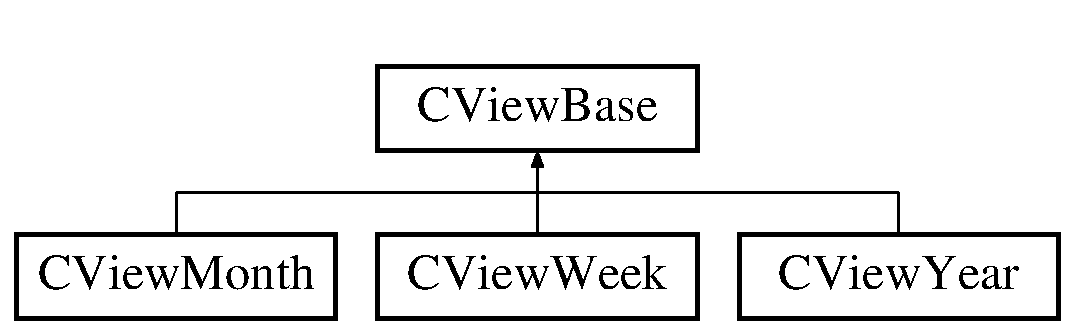
\includegraphics[height=2.000000cm]{class_c_view_base}
\end{center}
\end{figure}
\subsection*{Public Member Functions}
\begin{DoxyCompactItemize}
\item 
virtual \mbox{\hyperlink{class_c_view_base_ae4d24781c607bf3c22923c7cd40e1943}{$\sim$\+C\+View\+Base}} ()=default
\item 
virtual void \mbox{\hyperlink{class_c_view_base_a10a44a3680cc7ba6cd42ed99d128ed22}{Draw}} (const \mbox{\hyperlink{class_c_calendar}{C\+Calendar}} \&calendar, const \mbox{\hyperlink{class_c_date}{C\+Date}} \&date) const =0
\item 
virtual \mbox{\hyperlink{class_c_date}{C\+Date}} \mbox{\hyperlink{class_c_view_base_a9f5365e3225fb1b96058a9f8a599db6b}{Previous}} (const \mbox{\hyperlink{class_c_date}{C\+Date}} \&date) const =0
\item 
virtual \mbox{\hyperlink{class_c_date}{C\+Date}} \mbox{\hyperlink{class_c_view_base_afac2271f0a54dfa083246d4e9c3d0742}{Next}} (const \mbox{\hyperlink{class_c_date}{C\+Date}} \&date) const =0
\end{DoxyCompactItemize}


\subsection{Constructor \& Destructor Documentation}
\mbox{\Hypertarget{class_c_view_base_ae4d24781c607bf3c22923c7cd40e1943}\label{class_c_view_base_ae4d24781c607bf3c22923c7cd40e1943}} 
\index{C\+View\+Base@{C\+View\+Base}!````~C\+View\+Base@{$\sim$\+C\+View\+Base}}
\index{````~C\+View\+Base@{$\sim$\+C\+View\+Base}!C\+View\+Base@{C\+View\+Base}}
\subsubsection{\texorpdfstring{$\sim$\+C\+View\+Base()}{~CViewBase()}}
{\footnotesize\ttfamily virtual C\+View\+Base\+::$\sim$\+C\+View\+Base (\begin{DoxyParamCaption}{ }\end{DoxyParamCaption})\hspace{0.3cm}{\ttfamily [virtual]}, {\ttfamily [default]}}



\subsection{Member Function Documentation}
\mbox{\Hypertarget{class_c_view_base_a10a44a3680cc7ba6cd42ed99d128ed22}\label{class_c_view_base_a10a44a3680cc7ba6cd42ed99d128ed22}} 
\index{C\+View\+Base@{C\+View\+Base}!Draw@{Draw}}
\index{Draw@{Draw}!C\+View\+Base@{C\+View\+Base}}
\subsubsection{\texorpdfstring{Draw()}{Draw()}}
{\footnotesize\ttfamily virtual void C\+View\+Base\+::\+Draw (\begin{DoxyParamCaption}\item[{const \mbox{\hyperlink{class_c_calendar}{C\+Calendar}} \&}]{calendar,  }\item[{const \mbox{\hyperlink{class_c_date}{C\+Date}} \&}]{date }\end{DoxyParamCaption}) const\hspace{0.3cm}{\ttfamily [pure virtual]}}



Implemented in \mbox{\hyperlink{class_c_view_year_ad8f7c1b95dc1e46ae842f9e36aff6669}{C\+View\+Year}}, and \mbox{\hyperlink{class_c_view_month_acfed5c2bd785ee77f5528539a46f743c}{C\+View\+Month}}.

\mbox{\Hypertarget{class_c_view_base_afac2271f0a54dfa083246d4e9c3d0742}\label{class_c_view_base_afac2271f0a54dfa083246d4e9c3d0742}} 
\index{C\+View\+Base@{C\+View\+Base}!Next@{Next}}
\index{Next@{Next}!C\+View\+Base@{C\+View\+Base}}
\subsubsection{\texorpdfstring{Next()}{Next()}}
{\footnotesize\ttfamily virtual \mbox{\hyperlink{class_c_date}{C\+Date}} C\+View\+Base\+::\+Next (\begin{DoxyParamCaption}\item[{const \mbox{\hyperlink{class_c_date}{C\+Date}} \&}]{date }\end{DoxyParamCaption}) const\hspace{0.3cm}{\ttfamily [pure virtual]}}



Implemented in \mbox{\hyperlink{class_c_view_year_a93c8851786eac9fffe55cf006965a505}{C\+View\+Year}}, and \mbox{\hyperlink{class_c_view_month_a61677174b4ffadff768792deeef52b5e}{C\+View\+Month}}.

\mbox{\Hypertarget{class_c_view_base_a9f5365e3225fb1b96058a9f8a599db6b}\label{class_c_view_base_a9f5365e3225fb1b96058a9f8a599db6b}} 
\index{C\+View\+Base@{C\+View\+Base}!Previous@{Previous}}
\index{Previous@{Previous}!C\+View\+Base@{C\+View\+Base}}
\subsubsection{\texorpdfstring{Previous()}{Previous()}}
{\footnotesize\ttfamily virtual \mbox{\hyperlink{class_c_date}{C\+Date}} C\+View\+Base\+::\+Previous (\begin{DoxyParamCaption}\item[{const \mbox{\hyperlink{class_c_date}{C\+Date}} \&}]{date }\end{DoxyParamCaption}) const\hspace{0.3cm}{\ttfamily [pure virtual]}}



Implemented in \mbox{\hyperlink{class_c_view_year_a638b9541c8e0396a263bcff37a126f81}{C\+View\+Year}}, and \mbox{\hyperlink{class_c_view_month_ad945457c5bf0dbd491facee6a0852714}{C\+View\+Month}}.



The documentation for this class was generated from the following file\+:\begin{DoxyCompactItemize}
\item 
U\+I/\mbox{\hyperlink{_c_view_base_8h}{C\+View\+Base.\+h}}\end{DoxyCompactItemize}

\hypertarget{class_c_view_day}{}\section{C\+View\+Day Class Reference}
\label{class_c_view_day}\index{C\+View\+Day@{C\+View\+Day}}


{\ttfamily \#include $<$C\+View\+Day.\+h$>$}



The documentation for this class was generated from the following file\+:\begin{DoxyCompactItemize}
\item 
U\+I/\mbox{\hyperlink{_c_view_day_8h}{C\+View\+Day.\+h}}\end{DoxyCompactItemize}

\hypertarget{class_c_view_month}{}\section{C\+View\+Month Class Reference}
\label{class_c_view_month}\index{C\+View\+Month@{C\+View\+Month}}


{\ttfamily \#include $<$C\+View\+Month.\+h$>$}

Inheritance diagram for C\+View\+Month\+:\begin{figure}[H]
\begin{center}
\leavevmode
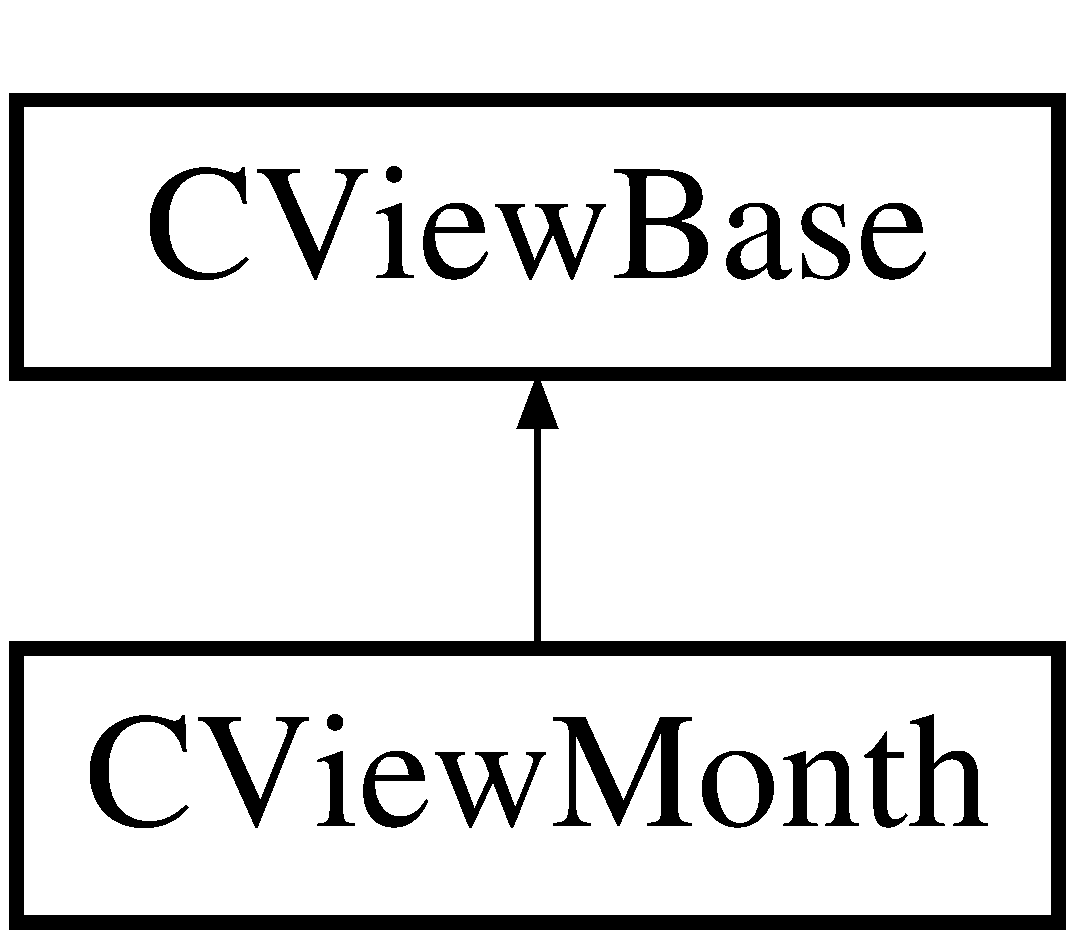
\includegraphics[height=2.000000cm]{class_c_view_month}
\end{center}
\end{figure}
\subsection*{Public Member Functions}
\begin{DoxyCompactItemize}
\item 
\mbox{\hyperlink{class_c_view_month_afaa51a2b2d21e1765618d10c56fa8fcd}{$\sim$\+C\+View\+Month}} ()=default
\item 
void \mbox{\hyperlink{class_c_view_month_acfed5c2bd785ee77f5528539a46f743c}{Draw}} (const \mbox{\hyperlink{class_c_calendar}{C\+Calendar}} \&calendar, const \mbox{\hyperlink{class_c_date}{C\+Date}} \&date) const override
\item 
\mbox{\hyperlink{class_c_date}{C\+Date}} \mbox{\hyperlink{class_c_view_month_ad945457c5bf0dbd491facee6a0852714}{Previous}} (const \mbox{\hyperlink{class_c_date}{C\+Date}} \&date) const override
\item 
\mbox{\hyperlink{class_c_date}{C\+Date}} \mbox{\hyperlink{class_c_view_month_a61677174b4ffadff768792deeef52b5e}{Next}} (const \mbox{\hyperlink{class_c_date}{C\+Date}} \&date) const override
\end{DoxyCompactItemize}


\subsection{Constructor \& Destructor Documentation}
\mbox{\Hypertarget{class_c_view_month_afaa51a2b2d21e1765618d10c56fa8fcd}\label{class_c_view_month_afaa51a2b2d21e1765618d10c56fa8fcd}} 
\index{C\+View\+Month@{C\+View\+Month}!````~C\+View\+Month@{$\sim$\+C\+View\+Month}}
\index{````~C\+View\+Month@{$\sim$\+C\+View\+Month}!C\+View\+Month@{C\+View\+Month}}
\subsubsection{\texorpdfstring{$\sim$\+C\+View\+Month()}{~CViewMonth()}}
{\footnotesize\ttfamily C\+View\+Month\+::$\sim$\+C\+View\+Month (\begin{DoxyParamCaption}{ }\end{DoxyParamCaption})\hspace{0.3cm}{\ttfamily [default]}}



\subsection{Member Function Documentation}
\mbox{\Hypertarget{class_c_view_month_acfed5c2bd785ee77f5528539a46f743c}\label{class_c_view_month_acfed5c2bd785ee77f5528539a46f743c}} 
\index{C\+View\+Month@{C\+View\+Month}!Draw@{Draw}}
\index{Draw@{Draw}!C\+View\+Month@{C\+View\+Month}}
\subsubsection{\texorpdfstring{Draw()}{Draw()}}
{\footnotesize\ttfamily void C\+View\+Month\+::\+Draw (\begin{DoxyParamCaption}\item[{const \mbox{\hyperlink{class_c_calendar}{C\+Calendar}} \&}]{calendar,  }\item[{const \mbox{\hyperlink{class_c_date}{C\+Date}} \&}]{date }\end{DoxyParamCaption}) const\hspace{0.3cm}{\ttfamily [override]}, {\ttfamily [virtual]}}



Implements \mbox{\hyperlink{class_c_view_base_a10a44a3680cc7ba6cd42ed99d128ed22}{C\+View\+Base}}.

\mbox{\Hypertarget{class_c_view_month_a61677174b4ffadff768792deeef52b5e}\label{class_c_view_month_a61677174b4ffadff768792deeef52b5e}} 
\index{C\+View\+Month@{C\+View\+Month}!Next@{Next}}
\index{Next@{Next}!C\+View\+Month@{C\+View\+Month}}
\subsubsection{\texorpdfstring{Next()}{Next()}}
{\footnotesize\ttfamily \mbox{\hyperlink{class_c_date}{C\+Date}} C\+View\+Month\+::\+Next (\begin{DoxyParamCaption}\item[{const \mbox{\hyperlink{class_c_date}{C\+Date}} \&}]{date }\end{DoxyParamCaption}) const\hspace{0.3cm}{\ttfamily [override]}, {\ttfamily [virtual]}}



Implements \mbox{\hyperlink{class_c_view_base_afac2271f0a54dfa083246d4e9c3d0742}{C\+View\+Base}}.

\mbox{\Hypertarget{class_c_view_month_ad945457c5bf0dbd491facee6a0852714}\label{class_c_view_month_ad945457c5bf0dbd491facee6a0852714}} 
\index{C\+View\+Month@{C\+View\+Month}!Previous@{Previous}}
\index{Previous@{Previous}!C\+View\+Month@{C\+View\+Month}}
\subsubsection{\texorpdfstring{Previous()}{Previous()}}
{\footnotesize\ttfamily \mbox{\hyperlink{class_c_date}{C\+Date}} C\+View\+Month\+::\+Previous (\begin{DoxyParamCaption}\item[{const \mbox{\hyperlink{class_c_date}{C\+Date}} \&}]{date }\end{DoxyParamCaption}) const\hspace{0.3cm}{\ttfamily [override]}, {\ttfamily [virtual]}}



Implements \mbox{\hyperlink{class_c_view_base_a9f5365e3225fb1b96058a9f8a599db6b}{C\+View\+Base}}.



The documentation for this class was generated from the following files\+:\begin{DoxyCompactItemize}
\item 
U\+I/\mbox{\hyperlink{_c_view_month_8h}{C\+View\+Month.\+h}}\item 
U\+I/\mbox{\hyperlink{_c_view_month_8cpp}{C\+View\+Month.\+cpp}}\end{DoxyCompactItemize}

\hypertarget{class_c_view_week}{}\section{C\+View\+Week Class Reference}
\label{class_c_view_week}\index{C\+View\+Week@{C\+View\+Week}}


{\ttfamily \#include $<$C\+View\+Week.\+h$>$}

Inheritance diagram for C\+View\+Week\+:\begin{figure}[H]
\begin{center}
\leavevmode
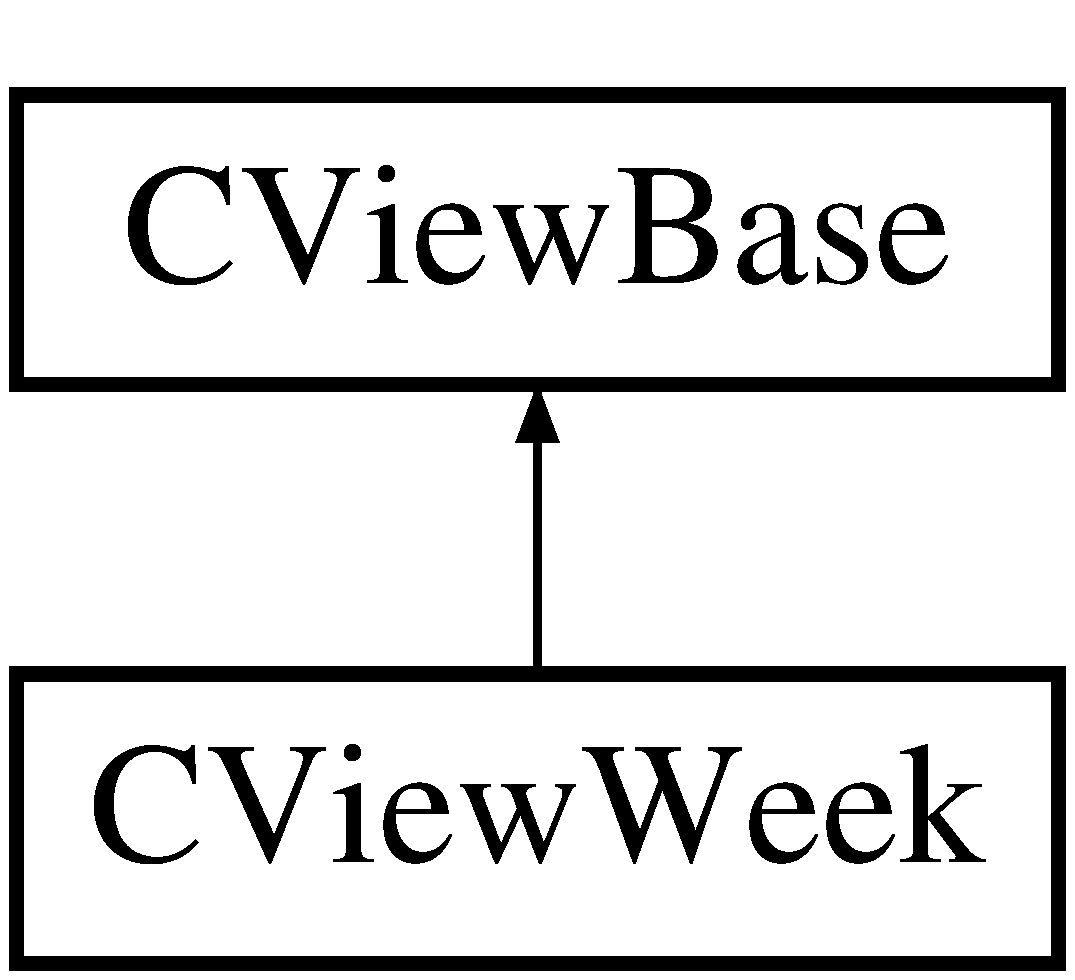
\includegraphics[height=2.000000cm]{class_c_view_week}
\end{center}
\end{figure}
\subsection*{Additional Inherited Members}


The documentation for this class was generated from the following files\+:\begin{DoxyCompactItemize}
\item 
U\+I/\mbox{\hyperlink{_c_view_week_8h}{C\+View\+Week.\+h}}\item 
U\+I/\mbox{\hyperlink{_c_view_week_8cpp}{C\+View\+Week.\+cpp}}\end{DoxyCompactItemize}

\hypertarget{class_c_view_year}{}\section{C\+View\+Year Class Reference}
\label{class_c_view_year}\index{C\+View\+Year@{C\+View\+Year}}


{\ttfamily \#include $<$C\+View\+Year.\+h$>$}

Inheritance diagram for C\+View\+Year\+:\begin{figure}[H]
\begin{center}
\leavevmode
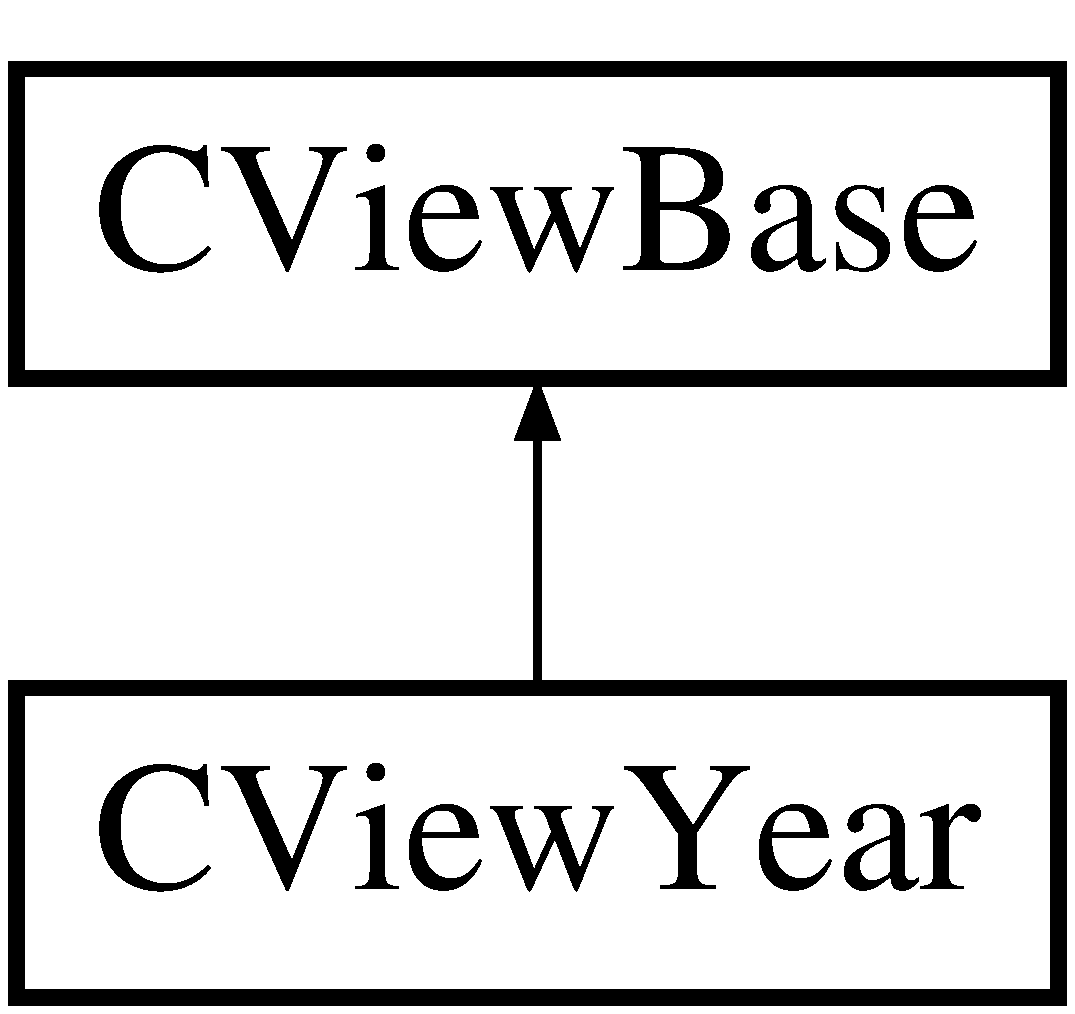
\includegraphics[height=2.000000cm]{class_c_view_year}
\end{center}
\end{figure}
\subsection*{Public Member Functions}
\begin{DoxyCompactItemize}
\item 
\mbox{\hyperlink{class_c_view_year_ac69be96e6e14d86bf4507e4a549e1710}{$\sim$\+C\+View\+Year}} ()=default
\item 
void \mbox{\hyperlink{class_c_view_year_ad8f7c1b95dc1e46ae842f9e36aff6669}{Draw}} (const \mbox{\hyperlink{class_c_calendar}{C\+Calendar}} \&calendar, const \mbox{\hyperlink{class_c_date}{C\+Date}} \&date) const override
\item 
\mbox{\hyperlink{class_c_date}{C\+Date}} \mbox{\hyperlink{class_c_view_year_a638b9541c8e0396a263bcff37a126f81}{Previous}} (const \mbox{\hyperlink{class_c_date}{C\+Date}} \&date) const override
\item 
\mbox{\hyperlink{class_c_date}{C\+Date}} \mbox{\hyperlink{class_c_view_year_a93c8851786eac9fffe55cf006965a505}{Next}} (const \mbox{\hyperlink{class_c_date}{C\+Date}} \&date) const override
\end{DoxyCompactItemize}


\subsection{Constructor \& Destructor Documentation}
\mbox{\Hypertarget{class_c_view_year_ac69be96e6e14d86bf4507e4a549e1710}\label{class_c_view_year_ac69be96e6e14d86bf4507e4a549e1710}} 
\index{C\+View\+Year@{C\+View\+Year}!````~C\+View\+Year@{$\sim$\+C\+View\+Year}}
\index{````~C\+View\+Year@{$\sim$\+C\+View\+Year}!C\+View\+Year@{C\+View\+Year}}
\subsubsection{\texorpdfstring{$\sim$\+C\+View\+Year()}{~CViewYear()}}
{\footnotesize\ttfamily C\+View\+Year\+::$\sim$\+C\+View\+Year (\begin{DoxyParamCaption}{ }\end{DoxyParamCaption})\hspace{0.3cm}{\ttfamily [default]}}



\subsection{Member Function Documentation}
\mbox{\Hypertarget{class_c_view_year_ad8f7c1b95dc1e46ae842f9e36aff6669}\label{class_c_view_year_ad8f7c1b95dc1e46ae842f9e36aff6669}} 
\index{C\+View\+Year@{C\+View\+Year}!Draw@{Draw}}
\index{Draw@{Draw}!C\+View\+Year@{C\+View\+Year}}
\subsubsection{\texorpdfstring{Draw()}{Draw()}}
{\footnotesize\ttfamily void C\+View\+Year\+::\+Draw (\begin{DoxyParamCaption}\item[{const \mbox{\hyperlink{class_c_calendar}{C\+Calendar}} \&}]{calendar,  }\item[{const \mbox{\hyperlink{class_c_date}{C\+Date}} \&}]{date }\end{DoxyParamCaption}) const\hspace{0.3cm}{\ttfamily [override]}, {\ttfamily [virtual]}}



Implements \mbox{\hyperlink{class_c_view_base_a10a44a3680cc7ba6cd42ed99d128ed22}{C\+View\+Base}}.

\mbox{\Hypertarget{class_c_view_year_a93c8851786eac9fffe55cf006965a505}\label{class_c_view_year_a93c8851786eac9fffe55cf006965a505}} 
\index{C\+View\+Year@{C\+View\+Year}!Next@{Next}}
\index{Next@{Next}!C\+View\+Year@{C\+View\+Year}}
\subsubsection{\texorpdfstring{Next()}{Next()}}
{\footnotesize\ttfamily \mbox{\hyperlink{class_c_date}{C\+Date}} C\+View\+Year\+::\+Next (\begin{DoxyParamCaption}\item[{const \mbox{\hyperlink{class_c_date}{C\+Date}} \&}]{date }\end{DoxyParamCaption}) const\hspace{0.3cm}{\ttfamily [override]}, {\ttfamily [virtual]}}



Implements \mbox{\hyperlink{class_c_view_base_afac2271f0a54dfa083246d4e9c3d0742}{C\+View\+Base}}.

\mbox{\Hypertarget{class_c_view_year_a638b9541c8e0396a263bcff37a126f81}\label{class_c_view_year_a638b9541c8e0396a263bcff37a126f81}} 
\index{C\+View\+Year@{C\+View\+Year}!Previous@{Previous}}
\index{Previous@{Previous}!C\+View\+Year@{C\+View\+Year}}
\subsubsection{\texorpdfstring{Previous()}{Previous()}}
{\footnotesize\ttfamily \mbox{\hyperlink{class_c_date}{C\+Date}} C\+View\+Year\+::\+Previous (\begin{DoxyParamCaption}\item[{const \mbox{\hyperlink{class_c_date}{C\+Date}} \&}]{date }\end{DoxyParamCaption}) const\hspace{0.3cm}{\ttfamily [override]}, {\ttfamily [virtual]}}



Implements \mbox{\hyperlink{class_c_view_base_a9f5365e3225fb1b96058a9f8a599db6b}{C\+View\+Base}}.



The documentation for this class was generated from the following files\+:\begin{DoxyCompactItemize}
\item 
U\+I/\mbox{\hyperlink{_c_view_year_8h}{C\+View\+Year.\+h}}\item 
U\+I/\mbox{\hyperlink{_c_view_year_8cpp}{C\+View\+Year.\+cpp}}\end{DoxyCompactItemize}

\hypertarget{class_empty_line_exception}{}\section{Empty\+Line\+Exception Class Reference}
\label{class_empty_line_exception}\index{Empty\+Line\+Exception@{Empty\+Line\+Exception}}


{\ttfamily \#include $<$utils.\+h$>$}



\subsection{Detailed Description}
Thrown in some cases when stream has empy line in it. 

The documentation for this class was generated from the following file\+:\begin{DoxyCompactItemize}
\item 
utils/\mbox{\hyperlink{utils_8h}{utils.\+h}}\end{DoxyCompactItemize}

\hypertarget{struct_c_event_1_1_get_searchable}{}\section{C\+Event\+:\+:Get\+Searchable Struct Reference}
\label{struct_c_event_1_1_get_searchable}\index{C\+Event\+::\+Get\+Searchable@{C\+Event\+::\+Get\+Searchable}}


{\ttfamily \#include $<$C\+Event.\+h$>$}

\subsection*{Public Member Functions}
\begin{DoxyCompactItemize}
\item 
std\+::vector$<$ std\+::string $>$ \mbox{\hyperlink{struct_c_event_1_1_get_searchable_a0a63d28071344813d360cd4cff268fab}{operator()}} (\mbox{\hyperlink{class_c_event}{C\+Event}} $\ast$const \&ev) const
\end{DoxyCompactItemize}


\subsection{Member Function Documentation}
\mbox{\Hypertarget{struct_c_event_1_1_get_searchable_a0a63d28071344813d360cd4cff268fab}\label{struct_c_event_1_1_get_searchable_a0a63d28071344813d360cd4cff268fab}} 
\index{C\+Event\+::\+Get\+Searchable@{C\+Event\+::\+Get\+Searchable}!operator()@{operator()}}
\index{operator()@{operator()}!C\+Event\+::\+Get\+Searchable@{C\+Event\+::\+Get\+Searchable}}
\subsubsection{\texorpdfstring{operator()()}{operator()()}}
{\footnotesize\ttfamily std\+::vector$<$ std\+::string $>$ C\+Event\+::\+Get\+Searchable\+::operator() (\begin{DoxyParamCaption}\item[{\mbox{\hyperlink{class_c_event}{C\+Event}} $\ast$const \&}]{ev }\end{DoxyParamCaption}) const}



The documentation for this struct was generated from the following files\+:\begin{DoxyCompactItemize}
\item 
Event/\mbox{\hyperlink{_c_event_8h}{C\+Event.\+h}}\item 
Event/\mbox{\hyperlink{_c_event_8cpp}{C\+Event.\+cpp}}\end{DoxyCompactItemize}

\hypertarget{struct_c_duration_1_1_separated}{}\section{C\+Duration\+:\+:Separated Struct Reference}
\label{struct_c_duration_1_1_separated}\index{C\+Duration\+::\+Separated@{C\+Duration\+::\+Separated}}


{\ttfamily \#include $<$C\+Duration.\+h$>$}

\subsection*{Public Attributes}
\begin{DoxyCompactItemize}
\item 
long long int \mbox{\hyperlink{struct_c_duration_1_1_separated_acbdcab6679092f3db70f9bc804757764}{years}}
\item 
long long int \mbox{\hyperlink{struct_c_duration_1_1_separated_afa838287265025d66478f6c2be9795b4}{months}}
\item 
long long int \mbox{\hyperlink{struct_c_duration_1_1_separated_ac4b83435c7d0e87d5335a20039b01753}{weeks}}
\item 
long long int \mbox{\hyperlink{struct_c_duration_1_1_separated_ac2dc46b006d0b613c72558c325a847c8}{days}}
\item 
long long int \mbox{\hyperlink{struct_c_duration_1_1_separated_a15c891acabf59f674ea756cc8a567d06}{hours}}
\item 
long long int \mbox{\hyperlink{struct_c_duration_1_1_separated_ab5def9b56f227359f798fe02d1b688ca}{minutes}}
\item 
long long int \mbox{\hyperlink{struct_c_duration_1_1_separated_ae3682ffed4c8577cd77185ace9d21fcf}{seconds}}
\end{DoxyCompactItemize}


\subsection{Member Data Documentation}
\mbox{\Hypertarget{struct_c_duration_1_1_separated_ac2dc46b006d0b613c72558c325a847c8}\label{struct_c_duration_1_1_separated_ac2dc46b006d0b613c72558c325a847c8}} 
\index{C\+Duration\+::\+Separated@{C\+Duration\+::\+Separated}!days@{days}}
\index{days@{days}!C\+Duration\+::\+Separated@{C\+Duration\+::\+Separated}}
\subsubsection{\texorpdfstring{days}{days}}
{\footnotesize\ttfamily long long int C\+Duration\+::\+Separated\+::days}

\mbox{\Hypertarget{struct_c_duration_1_1_separated_a15c891acabf59f674ea756cc8a567d06}\label{struct_c_duration_1_1_separated_a15c891acabf59f674ea756cc8a567d06}} 
\index{C\+Duration\+::\+Separated@{C\+Duration\+::\+Separated}!hours@{hours}}
\index{hours@{hours}!C\+Duration\+::\+Separated@{C\+Duration\+::\+Separated}}
\subsubsection{\texorpdfstring{hours}{hours}}
{\footnotesize\ttfamily long long int C\+Duration\+::\+Separated\+::hours}

\mbox{\Hypertarget{struct_c_duration_1_1_separated_ab5def9b56f227359f798fe02d1b688ca}\label{struct_c_duration_1_1_separated_ab5def9b56f227359f798fe02d1b688ca}} 
\index{C\+Duration\+::\+Separated@{C\+Duration\+::\+Separated}!minutes@{minutes}}
\index{minutes@{minutes}!C\+Duration\+::\+Separated@{C\+Duration\+::\+Separated}}
\subsubsection{\texorpdfstring{minutes}{minutes}}
{\footnotesize\ttfamily long long int C\+Duration\+::\+Separated\+::minutes}

\mbox{\Hypertarget{struct_c_duration_1_1_separated_afa838287265025d66478f6c2be9795b4}\label{struct_c_duration_1_1_separated_afa838287265025d66478f6c2be9795b4}} 
\index{C\+Duration\+::\+Separated@{C\+Duration\+::\+Separated}!months@{months}}
\index{months@{months}!C\+Duration\+::\+Separated@{C\+Duration\+::\+Separated}}
\subsubsection{\texorpdfstring{months}{months}}
{\footnotesize\ttfamily long long int C\+Duration\+::\+Separated\+::months}

\mbox{\Hypertarget{struct_c_duration_1_1_separated_ae3682ffed4c8577cd77185ace9d21fcf}\label{struct_c_duration_1_1_separated_ae3682ffed4c8577cd77185ace9d21fcf}} 
\index{C\+Duration\+::\+Separated@{C\+Duration\+::\+Separated}!seconds@{seconds}}
\index{seconds@{seconds}!C\+Duration\+::\+Separated@{C\+Duration\+::\+Separated}}
\subsubsection{\texorpdfstring{seconds}{seconds}}
{\footnotesize\ttfamily long long int C\+Duration\+::\+Separated\+::seconds}

\mbox{\Hypertarget{struct_c_duration_1_1_separated_ac4b83435c7d0e87d5335a20039b01753}\label{struct_c_duration_1_1_separated_ac4b83435c7d0e87d5335a20039b01753}} 
\index{C\+Duration\+::\+Separated@{C\+Duration\+::\+Separated}!weeks@{weeks}}
\index{weeks@{weeks}!C\+Duration\+::\+Separated@{C\+Duration\+::\+Separated}}
\subsubsection{\texorpdfstring{weeks}{weeks}}
{\footnotesize\ttfamily long long int C\+Duration\+::\+Separated\+::weeks}

\mbox{\Hypertarget{struct_c_duration_1_1_separated_acbdcab6679092f3db70f9bc804757764}\label{struct_c_duration_1_1_separated_acbdcab6679092f3db70f9bc804757764}} 
\index{C\+Duration\+::\+Separated@{C\+Duration\+::\+Separated}!years@{years}}
\index{years@{years}!C\+Duration\+::\+Separated@{C\+Duration\+::\+Separated}}
\subsubsection{\texorpdfstring{years}{years}}
{\footnotesize\ttfamily long long int C\+Duration\+::\+Separated\+::years}



The documentation for this struct was generated from the following file\+:\begin{DoxyCompactItemize}
\item 
Date/\mbox{\hyperlink{_c_duration_8h}{C\+Duration.\+h}}\end{DoxyCompactItemize}

\chapter{File Documentation}
\hypertarget{_c_calendar_8cpp}{}\section{Calendar/\+C\+Calendar.cpp File Reference}
\label{_c_calendar_8cpp}\index{Calendar/\+C\+Calendar.\+cpp@{Calendar/\+C\+Calendar.\+cpp}}
{\ttfamily \#include $<$vector$>$}\newline
{\ttfamily \#include \char`\"{}C\+Calendar.\+h\char`\"{}}\newline
{\ttfamily \#include \char`\"{}../utils/utils.\+h\char`\"{}}\newline

\hypertarget{_c_calendar_8h}{}\section{Calendar/\+C\+Calendar.h File Reference}
\label{_c_calendar_8h}\index{Calendar/\+C\+Calendar.\+h@{Calendar/\+C\+Calendar.\+h}}
{\ttfamily \#include $<$vector$>$}\newline
{\ttfamily \#include $<$string$>$}\newline
{\ttfamily \#include \char`\"{}../utils/\+C\+Suggestor.\+h\char`\"{}}\newline
{\ttfamily \#include \char`\"{}../\+Event/\+C\+Event.\+h\char`\"{}}\newline
\subsection*{Classes}
\begin{DoxyCompactItemize}
\item 
class \mbox{\hyperlink{class_c_calendar}{C\+Calendar}}
\end{DoxyCompactItemize}

\hypertarget{_c_make_c_compiler_id_8c}{}\section{cmake-\/build-\/debug/\+C\+Make\+Files/3.8.2/\+Compiler\+Id\+C/\+C\+Make\+C\+Compiler\+Id.c File Reference}
\label{_c_make_c_compiler_id_8c}\index{cmake-\/build-\/debug/\+C\+Make\+Files/3.\+8.\+2/\+Compiler\+Id\+C/\+C\+Make\+C\+Compiler\+Id.\+c@{cmake-\/build-\/debug/\+C\+Make\+Files/3.\+8.\+2/\+Compiler\+Id\+C/\+C\+Make\+C\+Compiler\+Id.\+c}}
\subsection*{Macros}
\begin{DoxyCompactItemize}
\item 
\#define \mbox{\hyperlink{_c_make_c_compiler_id_8c_a81dee0709ded976b2e0319239f72d174}{C\+O\+M\+P\+I\+L\+E\+R\+\_\+\+ID}}~\char`\"{}\char`\"{}
\item 
\#define \mbox{\hyperlink{_c_make_c_compiler_id_8c_a2ae9b72bb13abaabfcf2ee0ba7d3fa1d}{S\+T\+R\+I\+N\+G\+I\+F\+Y\+\_\+\+H\+E\+L\+P\+ER}}(X)~\#X
\item 
\#define \mbox{\hyperlink{_c_make_c_compiler_id_8c_a43e1cad902b6477bec893cb6430bd6c8}{S\+T\+R\+I\+N\+G\+I\+FY}}(X)~\mbox{\hyperlink{_c_make_c_x_x_compiler_id_8cpp_a2ae9b72bb13abaabfcf2ee0ba7d3fa1d}{S\+T\+R\+I\+N\+G\+I\+F\+Y\+\_\+\+H\+E\+L\+P\+ER}}(X)
\item 
\#define \mbox{\hyperlink{_c_make_c_compiler_id_8c_adbc5372f40838899018fadbc89bd588b}{P\+L\+A\+T\+F\+O\+R\+M\+\_\+\+ID}}
\item 
\#define \mbox{\hyperlink{_c_make_c_compiler_id_8c_aba35d0d200deaeb06aee95ca297acb28}{A\+R\+C\+H\+I\+T\+E\+C\+T\+U\+R\+E\+\_\+\+ID}}
\item 
\#define \mbox{\hyperlink{_c_make_c_compiler_id_8c_ad1280362da42492bbc11aa78cbf776ad}{D\+EC}}(n)
\item 
\#define \mbox{\hyperlink{_c_make_c_compiler_id_8c_a46d5d95daa1bef867bd0179594310ed5}{H\+EX}}(n)
\item 
\#define \mbox{\hyperlink{_c_make_c_compiler_id_8c_a07f8e5783674099cd7f5110e22a78cdb}{C\+\_\+\+D\+I\+A\+L\+E\+CT}}
\end{DoxyCompactItemize}
\subsection*{Functions}
\begin{DoxyCompactItemize}
\item 
int \mbox{\hyperlink{_c_make_c_compiler_id_8c_a0ddf1224851353fc92bfbff6f499fa97}{main}} (int argc, char $\ast$argv\mbox{[}$\,$\mbox{]})
\end{DoxyCompactItemize}
\subsection*{Variables}
\begin{DoxyCompactItemize}
\item 
char const  $\ast$ \mbox{\hyperlink{_c_make_c_compiler_id_8c_a4b0efeb7a5d59313986b3a0390f050f6}{info\+\_\+compiler}} = \char`\"{}I\+N\+FO\char`\"{} \char`\"{}\+:\char`\"{} \char`\"{}compiler\mbox{[}\char`\"{} C\+O\+M\+P\+I\+L\+E\+R\+\_\+\+ID \char`\"{}\mbox{]}\char`\"{}
\item 
char const  $\ast$ \mbox{\hyperlink{_c_make_c_compiler_id_8c_a2321403dee54ee23f0c2fa849c60f7d4}{info\+\_\+platform}} = \char`\"{}I\+N\+FO\char`\"{} \char`\"{}\+:\char`\"{} \char`\"{}platform\mbox{[}\char`\"{} P\+L\+A\+T\+F\+O\+R\+M\+\_\+\+ID \char`\"{}\mbox{]}\char`\"{}
\item 
char const  $\ast$ \mbox{\hyperlink{_c_make_c_compiler_id_8c_a59647e99d304ed33b15cb284c27ed391}{info\+\_\+arch}} = \char`\"{}I\+N\+FO\char`\"{} \char`\"{}\+:\char`\"{} \char`\"{}arch\mbox{[}\char`\"{} A\+R\+C\+H\+I\+T\+E\+C\+T\+U\+R\+E\+\_\+\+ID \char`\"{}\mbox{]}\char`\"{}
\item 
const char $\ast$ \mbox{\hyperlink{_c_make_c_compiler_id_8c_a1ce162bad2fe6966ac8b33cc19e120b8}{info\+\_\+language\+\_\+dialect\+\_\+default}}
\end{DoxyCompactItemize}


\subsection{Macro Definition Documentation}
\mbox{\Hypertarget{_c_make_c_compiler_id_8c_aba35d0d200deaeb06aee95ca297acb28}\label{_c_make_c_compiler_id_8c_aba35d0d200deaeb06aee95ca297acb28}} 
\index{C\+Make\+C\+Compiler\+Id.\+c@{C\+Make\+C\+Compiler\+Id.\+c}!A\+R\+C\+H\+I\+T\+E\+C\+T\+U\+R\+E\+\_\+\+ID@{A\+R\+C\+H\+I\+T\+E\+C\+T\+U\+R\+E\+\_\+\+ID}}
\index{A\+R\+C\+H\+I\+T\+E\+C\+T\+U\+R\+E\+\_\+\+ID@{A\+R\+C\+H\+I\+T\+E\+C\+T\+U\+R\+E\+\_\+\+ID}!C\+Make\+C\+Compiler\+Id.\+c@{C\+Make\+C\+Compiler\+Id.\+c}}
\subsubsection{\texorpdfstring{A\+R\+C\+H\+I\+T\+E\+C\+T\+U\+R\+E\+\_\+\+ID}{ARCHITECTURE\_ID}}
{\footnotesize\ttfamily \#define A\+R\+C\+H\+I\+T\+E\+C\+T\+U\+R\+E\+\_\+\+ID}

\mbox{\Hypertarget{_c_make_c_compiler_id_8c_a07f8e5783674099cd7f5110e22a78cdb}\label{_c_make_c_compiler_id_8c_a07f8e5783674099cd7f5110e22a78cdb}} 
\index{C\+Make\+C\+Compiler\+Id.\+c@{C\+Make\+C\+Compiler\+Id.\+c}!C\+\_\+\+D\+I\+A\+L\+E\+CT@{C\+\_\+\+D\+I\+A\+L\+E\+CT}}
\index{C\+\_\+\+D\+I\+A\+L\+E\+CT@{C\+\_\+\+D\+I\+A\+L\+E\+CT}!C\+Make\+C\+Compiler\+Id.\+c@{C\+Make\+C\+Compiler\+Id.\+c}}
\subsubsection{\texorpdfstring{C\+\_\+\+D\+I\+A\+L\+E\+CT}{C\_DIALECT}}
{\footnotesize\ttfamily \#define C\+\_\+\+D\+I\+A\+L\+E\+CT}

\mbox{\Hypertarget{_c_make_c_compiler_id_8c_a81dee0709ded976b2e0319239f72d174}\label{_c_make_c_compiler_id_8c_a81dee0709ded976b2e0319239f72d174}} 
\index{C\+Make\+C\+Compiler\+Id.\+c@{C\+Make\+C\+Compiler\+Id.\+c}!C\+O\+M\+P\+I\+L\+E\+R\+\_\+\+ID@{C\+O\+M\+P\+I\+L\+E\+R\+\_\+\+ID}}
\index{C\+O\+M\+P\+I\+L\+E\+R\+\_\+\+ID@{C\+O\+M\+P\+I\+L\+E\+R\+\_\+\+ID}!C\+Make\+C\+Compiler\+Id.\+c@{C\+Make\+C\+Compiler\+Id.\+c}}
\subsubsection{\texorpdfstring{C\+O\+M\+P\+I\+L\+E\+R\+\_\+\+ID}{COMPILER\_ID}}
{\footnotesize\ttfamily \#define C\+O\+M\+P\+I\+L\+E\+R\+\_\+\+ID~\char`\"{}\char`\"{}}

\mbox{\Hypertarget{_c_make_c_compiler_id_8c_ad1280362da42492bbc11aa78cbf776ad}\label{_c_make_c_compiler_id_8c_ad1280362da42492bbc11aa78cbf776ad}} 
\index{C\+Make\+C\+Compiler\+Id.\+c@{C\+Make\+C\+Compiler\+Id.\+c}!D\+EC@{D\+EC}}
\index{D\+EC@{D\+EC}!C\+Make\+C\+Compiler\+Id.\+c@{C\+Make\+C\+Compiler\+Id.\+c}}
\subsubsection{\texorpdfstring{D\+EC}{DEC}}
{\footnotesize\ttfamily \#define D\+EC(\begin{DoxyParamCaption}\item[{}]{n }\end{DoxyParamCaption})}

{\bfseries Value\+:}
\begin{DoxyCode}
(\textcolor{charliteral}{'0'} + (((n) / 10000000)%10)), \(\backslash\)
  (\textcolor{charliteral}{'0'} + (((n) / 1000000)%10)),  \(\backslash\)
  (\textcolor{charliteral}{'0'} + (((n) / 100000)%10)),   \(\backslash\)
  (\textcolor{charliteral}{'0'} + (((n) / 10000)%10)),    \(\backslash\)
  (\textcolor{charliteral}{'0'} + (((n) / 1000)%10)),     \(\backslash\)
  (\textcolor{charliteral}{'0'} + (((n) / 100)%10)),      \(\backslash\)
  (\textcolor{charliteral}{'0'} + (((n) / 10)%10)),       \(\backslash\)
  (\textcolor{charliteral}{'0'} +  ((n) % 10))
\end{DoxyCode}
\mbox{\Hypertarget{_c_make_c_compiler_id_8c_a46d5d95daa1bef867bd0179594310ed5}\label{_c_make_c_compiler_id_8c_a46d5d95daa1bef867bd0179594310ed5}} 
\index{C\+Make\+C\+Compiler\+Id.\+c@{C\+Make\+C\+Compiler\+Id.\+c}!H\+EX@{H\+EX}}
\index{H\+EX@{H\+EX}!C\+Make\+C\+Compiler\+Id.\+c@{C\+Make\+C\+Compiler\+Id.\+c}}
\subsubsection{\texorpdfstring{H\+EX}{HEX}}
{\footnotesize\ttfamily \#define H\+EX(\begin{DoxyParamCaption}\item[{}]{n }\end{DoxyParamCaption})}

{\bfseries Value\+:}
\begin{DoxyCode}
(\textcolor{charliteral}{'0'} + ((n)>>28 & 0xF)), \(\backslash\)
  (\textcolor{charliteral}{'0'} + ((n)>>24 & 0xF)), \(\backslash\)
  (\textcolor{charliteral}{'0'} + ((n)>>20 & 0xF)), \(\backslash\)
  (\textcolor{charliteral}{'0'} + ((n)>>16 & 0xF)), \(\backslash\)
  (\textcolor{charliteral}{'0'} + ((n)>>12 & 0xF)), \(\backslash\)
  (\textcolor{charliteral}{'0'} + ((n)>>8  & 0xF)), \(\backslash\)
  (\textcolor{charliteral}{'0'} + ((n)>>4  & 0xF)), \(\backslash\)
  (\textcolor{charliteral}{'0'} + ((n)     & 0xF))
\end{DoxyCode}
\mbox{\Hypertarget{_c_make_c_compiler_id_8c_adbc5372f40838899018fadbc89bd588b}\label{_c_make_c_compiler_id_8c_adbc5372f40838899018fadbc89bd588b}} 
\index{C\+Make\+C\+Compiler\+Id.\+c@{C\+Make\+C\+Compiler\+Id.\+c}!P\+L\+A\+T\+F\+O\+R\+M\+\_\+\+ID@{P\+L\+A\+T\+F\+O\+R\+M\+\_\+\+ID}}
\index{P\+L\+A\+T\+F\+O\+R\+M\+\_\+\+ID@{P\+L\+A\+T\+F\+O\+R\+M\+\_\+\+ID}!C\+Make\+C\+Compiler\+Id.\+c@{C\+Make\+C\+Compiler\+Id.\+c}}
\subsubsection{\texorpdfstring{P\+L\+A\+T\+F\+O\+R\+M\+\_\+\+ID}{PLATFORM\_ID}}
{\footnotesize\ttfamily \#define P\+L\+A\+T\+F\+O\+R\+M\+\_\+\+ID}

\mbox{\Hypertarget{_c_make_c_compiler_id_8c_a43e1cad902b6477bec893cb6430bd6c8}\label{_c_make_c_compiler_id_8c_a43e1cad902b6477bec893cb6430bd6c8}} 
\index{C\+Make\+C\+Compiler\+Id.\+c@{C\+Make\+C\+Compiler\+Id.\+c}!S\+T\+R\+I\+N\+G\+I\+FY@{S\+T\+R\+I\+N\+G\+I\+FY}}
\index{S\+T\+R\+I\+N\+G\+I\+FY@{S\+T\+R\+I\+N\+G\+I\+FY}!C\+Make\+C\+Compiler\+Id.\+c@{C\+Make\+C\+Compiler\+Id.\+c}}
\subsubsection{\texorpdfstring{S\+T\+R\+I\+N\+G\+I\+FY}{STRINGIFY}}
{\footnotesize\ttfamily \#define S\+T\+R\+I\+N\+G\+I\+FY(\begin{DoxyParamCaption}\item[{}]{X }\end{DoxyParamCaption})~\mbox{\hyperlink{_c_make_c_x_x_compiler_id_8cpp_a2ae9b72bb13abaabfcf2ee0ba7d3fa1d}{S\+T\+R\+I\+N\+G\+I\+F\+Y\+\_\+\+H\+E\+L\+P\+ER}}(X)}

\mbox{\Hypertarget{_c_make_c_compiler_id_8c_a2ae9b72bb13abaabfcf2ee0ba7d3fa1d}\label{_c_make_c_compiler_id_8c_a2ae9b72bb13abaabfcf2ee0ba7d3fa1d}} 
\index{C\+Make\+C\+Compiler\+Id.\+c@{C\+Make\+C\+Compiler\+Id.\+c}!S\+T\+R\+I\+N\+G\+I\+F\+Y\+\_\+\+H\+E\+L\+P\+ER@{S\+T\+R\+I\+N\+G\+I\+F\+Y\+\_\+\+H\+E\+L\+P\+ER}}
\index{S\+T\+R\+I\+N\+G\+I\+F\+Y\+\_\+\+H\+E\+L\+P\+ER@{S\+T\+R\+I\+N\+G\+I\+F\+Y\+\_\+\+H\+E\+L\+P\+ER}!C\+Make\+C\+Compiler\+Id.\+c@{C\+Make\+C\+Compiler\+Id.\+c}}
\subsubsection{\texorpdfstring{S\+T\+R\+I\+N\+G\+I\+F\+Y\+\_\+\+H\+E\+L\+P\+ER}{STRINGIFY\_HELPER}}
{\footnotesize\ttfamily \#define S\+T\+R\+I\+N\+G\+I\+F\+Y\+\_\+\+H\+E\+L\+P\+ER(\begin{DoxyParamCaption}\item[{}]{X }\end{DoxyParamCaption})~\#X}



\subsection{Function Documentation}
\mbox{\Hypertarget{_c_make_c_compiler_id_8c_a0ddf1224851353fc92bfbff6f499fa97}\label{_c_make_c_compiler_id_8c_a0ddf1224851353fc92bfbff6f499fa97}} 
\index{C\+Make\+C\+Compiler\+Id.\+c@{C\+Make\+C\+Compiler\+Id.\+c}!main@{main}}
\index{main@{main}!C\+Make\+C\+Compiler\+Id.\+c@{C\+Make\+C\+Compiler\+Id.\+c}}
\subsubsection{\texorpdfstring{main()}{main()}}
{\footnotesize\ttfamily int main (\begin{DoxyParamCaption}\item[{int}]{argc,  }\item[{char $\ast$}]{argv\mbox{[}$\,$\mbox{]} }\end{DoxyParamCaption})}



\subsection{Variable Documentation}
\mbox{\Hypertarget{_c_make_c_compiler_id_8c_a59647e99d304ed33b15cb284c27ed391}\label{_c_make_c_compiler_id_8c_a59647e99d304ed33b15cb284c27ed391}} 
\index{C\+Make\+C\+Compiler\+Id.\+c@{C\+Make\+C\+Compiler\+Id.\+c}!info\+\_\+arch@{info\+\_\+arch}}
\index{info\+\_\+arch@{info\+\_\+arch}!C\+Make\+C\+Compiler\+Id.\+c@{C\+Make\+C\+Compiler\+Id.\+c}}
\subsubsection{\texorpdfstring{info\+\_\+arch}{info\_arch}}
{\footnotesize\ttfamily char const$\ast$ info\+\_\+arch = \char`\"{}I\+N\+FO\char`\"{} \char`\"{}\+:\char`\"{} \char`\"{}arch\mbox{[}\char`\"{} A\+R\+C\+H\+I\+T\+E\+C\+T\+U\+R\+E\+\_\+\+ID \char`\"{}\mbox{]}\char`\"{}}

\mbox{\Hypertarget{_c_make_c_compiler_id_8c_a4b0efeb7a5d59313986b3a0390f050f6}\label{_c_make_c_compiler_id_8c_a4b0efeb7a5d59313986b3a0390f050f6}} 
\index{C\+Make\+C\+Compiler\+Id.\+c@{C\+Make\+C\+Compiler\+Id.\+c}!info\+\_\+compiler@{info\+\_\+compiler}}
\index{info\+\_\+compiler@{info\+\_\+compiler}!C\+Make\+C\+Compiler\+Id.\+c@{C\+Make\+C\+Compiler\+Id.\+c}}
\subsubsection{\texorpdfstring{info\+\_\+compiler}{info\_compiler}}
{\footnotesize\ttfamily char const$\ast$ info\+\_\+compiler = \char`\"{}I\+N\+FO\char`\"{} \char`\"{}\+:\char`\"{} \char`\"{}compiler\mbox{[}\char`\"{} C\+O\+M\+P\+I\+L\+E\+R\+\_\+\+ID \char`\"{}\mbox{]}\char`\"{}}

\mbox{\Hypertarget{_c_make_c_compiler_id_8c_a1ce162bad2fe6966ac8b33cc19e120b8}\label{_c_make_c_compiler_id_8c_a1ce162bad2fe6966ac8b33cc19e120b8}} 
\index{C\+Make\+C\+Compiler\+Id.\+c@{C\+Make\+C\+Compiler\+Id.\+c}!info\+\_\+language\+\_\+dialect\+\_\+default@{info\+\_\+language\+\_\+dialect\+\_\+default}}
\index{info\+\_\+language\+\_\+dialect\+\_\+default@{info\+\_\+language\+\_\+dialect\+\_\+default}!C\+Make\+C\+Compiler\+Id.\+c@{C\+Make\+C\+Compiler\+Id.\+c}}
\subsubsection{\texorpdfstring{info\+\_\+language\+\_\+dialect\+\_\+default}{info\_language\_dialect\_default}}
{\footnotesize\ttfamily const char$\ast$ info\+\_\+language\+\_\+dialect\+\_\+default}

{\bfseries Initial value\+:}
\begin{DoxyCode}
=
  \textcolor{stringliteral}{"INFO"} \textcolor{stringliteral}{":"} \textcolor{stringliteral}{"dialect\_default["} \mbox{\hyperlink{_c_make_c_compiler_id_8c_a07f8e5783674099cd7f5110e22a78cdb}{C\_DIALECT}} \textcolor{stringliteral}{"]"}
\end{DoxyCode}
\mbox{\Hypertarget{_c_make_c_compiler_id_8c_a2321403dee54ee23f0c2fa849c60f7d4}\label{_c_make_c_compiler_id_8c_a2321403dee54ee23f0c2fa849c60f7d4}} 
\index{C\+Make\+C\+Compiler\+Id.\+c@{C\+Make\+C\+Compiler\+Id.\+c}!info\+\_\+platform@{info\+\_\+platform}}
\index{info\+\_\+platform@{info\+\_\+platform}!C\+Make\+C\+Compiler\+Id.\+c@{C\+Make\+C\+Compiler\+Id.\+c}}
\subsubsection{\texorpdfstring{info\+\_\+platform}{info\_platform}}
{\footnotesize\ttfamily char const$\ast$ info\+\_\+platform = \char`\"{}I\+N\+FO\char`\"{} \char`\"{}\+:\char`\"{} \char`\"{}platform\mbox{[}\char`\"{} P\+L\+A\+T\+F\+O\+R\+M\+\_\+\+ID \char`\"{}\mbox{]}\char`\"{}}


\hypertarget{_c_make_c_x_x_compiler_id_8cpp}{}\section{cmake-\/build-\/debug/\+C\+Make\+Files/3.8.2/\+Compiler\+Id\+C\+X\+X/\+C\+Make\+C\+X\+X\+Compiler\+Id.cpp File Reference}
\label{_c_make_c_x_x_compiler_id_8cpp}\index{cmake-\/build-\/debug/\+C\+Make\+Files/3.\+8.\+2/\+Compiler\+Id\+C\+X\+X/\+C\+Make\+C\+X\+X\+Compiler\+Id.\+cpp@{cmake-\/build-\/debug/\+C\+Make\+Files/3.\+8.\+2/\+Compiler\+Id\+C\+X\+X/\+C\+Make\+C\+X\+X\+Compiler\+Id.\+cpp}}
\subsection*{Macros}
\begin{DoxyCompactItemize}
\item 
\#define \mbox{\hyperlink{_c_make_c_x_x_compiler_id_8cpp_a81dee0709ded976b2e0319239f72d174}{C\+O\+M\+P\+I\+L\+E\+R\+\_\+\+ID}}~\char`\"{}\char`\"{}
\item 
\#define \mbox{\hyperlink{_c_make_c_x_x_compiler_id_8cpp_a2ae9b72bb13abaabfcf2ee0ba7d3fa1d}{S\+T\+R\+I\+N\+G\+I\+F\+Y\+\_\+\+H\+E\+L\+P\+ER}}(X)~\#X
\item 
\#define \mbox{\hyperlink{_c_make_c_x_x_compiler_id_8cpp_a43e1cad902b6477bec893cb6430bd6c8}{S\+T\+R\+I\+N\+G\+I\+FY}}(X)~\mbox{\hyperlink{_c_make_c_x_x_compiler_id_8cpp_a2ae9b72bb13abaabfcf2ee0ba7d3fa1d}{S\+T\+R\+I\+N\+G\+I\+F\+Y\+\_\+\+H\+E\+L\+P\+ER}}(X)
\item 
\#define \mbox{\hyperlink{_c_make_c_x_x_compiler_id_8cpp_adbc5372f40838899018fadbc89bd588b}{P\+L\+A\+T\+F\+O\+R\+M\+\_\+\+ID}}
\item 
\#define \mbox{\hyperlink{_c_make_c_x_x_compiler_id_8cpp_aba35d0d200deaeb06aee95ca297acb28}{A\+R\+C\+H\+I\+T\+E\+C\+T\+U\+R\+E\+\_\+\+ID}}
\item 
\#define \mbox{\hyperlink{_c_make_c_x_x_compiler_id_8cpp_ad1280362da42492bbc11aa78cbf776ad}{D\+EC}}(n)
\item 
\#define \mbox{\hyperlink{_c_make_c_x_x_compiler_id_8cpp_a46d5d95daa1bef867bd0179594310ed5}{H\+EX}}(n)
\end{DoxyCompactItemize}
\subsection*{Functions}
\begin{DoxyCompactItemize}
\item 
int \mbox{\hyperlink{_c_make_c_x_x_compiler_id_8cpp_a0ddf1224851353fc92bfbff6f499fa97}{main}} (int argc, char $\ast$argv\mbox{[}$\,$\mbox{]})
\end{DoxyCompactItemize}
\subsection*{Variables}
\begin{DoxyCompactItemize}
\item 
char const  $\ast$ \mbox{\hyperlink{_c_make_c_x_x_compiler_id_8cpp_a4b0efeb7a5d59313986b3a0390f050f6}{info\+\_\+compiler}} = \char`\"{}I\+N\+FO\char`\"{} \char`\"{}\+:\char`\"{} \char`\"{}compiler\mbox{[}\char`\"{} C\+O\+M\+P\+I\+L\+E\+R\+\_\+\+ID \char`\"{}\mbox{]}\char`\"{}
\item 
char const  $\ast$ \mbox{\hyperlink{_c_make_c_x_x_compiler_id_8cpp_a2321403dee54ee23f0c2fa849c60f7d4}{info\+\_\+platform}} = \char`\"{}I\+N\+FO\char`\"{} \char`\"{}\+:\char`\"{} \char`\"{}platform\mbox{[}\char`\"{} P\+L\+A\+T\+F\+O\+R\+M\+\_\+\+ID \char`\"{}\mbox{]}\char`\"{}
\item 
char const  $\ast$ \mbox{\hyperlink{_c_make_c_x_x_compiler_id_8cpp_a59647e99d304ed33b15cb284c27ed391}{info\+\_\+arch}} = \char`\"{}I\+N\+FO\char`\"{} \char`\"{}\+:\char`\"{} \char`\"{}arch\mbox{[}\char`\"{} A\+R\+C\+H\+I\+T\+E\+C\+T\+U\+R\+E\+\_\+\+ID \char`\"{}\mbox{]}\char`\"{}
\item 
const char $\ast$ \mbox{\hyperlink{_c_make_c_x_x_compiler_id_8cpp_a1ce162bad2fe6966ac8b33cc19e120b8}{info\+\_\+language\+\_\+dialect\+\_\+default}}
\end{DoxyCompactItemize}


\subsection{Macro Definition Documentation}
\mbox{\Hypertarget{_c_make_c_x_x_compiler_id_8cpp_aba35d0d200deaeb06aee95ca297acb28}\label{_c_make_c_x_x_compiler_id_8cpp_aba35d0d200deaeb06aee95ca297acb28}} 
\index{C\+Make\+C\+X\+X\+Compiler\+Id.\+cpp@{C\+Make\+C\+X\+X\+Compiler\+Id.\+cpp}!A\+R\+C\+H\+I\+T\+E\+C\+T\+U\+R\+E\+\_\+\+ID@{A\+R\+C\+H\+I\+T\+E\+C\+T\+U\+R\+E\+\_\+\+ID}}
\index{A\+R\+C\+H\+I\+T\+E\+C\+T\+U\+R\+E\+\_\+\+ID@{A\+R\+C\+H\+I\+T\+E\+C\+T\+U\+R\+E\+\_\+\+ID}!C\+Make\+C\+X\+X\+Compiler\+Id.\+cpp@{C\+Make\+C\+X\+X\+Compiler\+Id.\+cpp}}
\subsubsection{\texorpdfstring{A\+R\+C\+H\+I\+T\+E\+C\+T\+U\+R\+E\+\_\+\+ID}{ARCHITECTURE\_ID}}
{\footnotesize\ttfamily \#define A\+R\+C\+H\+I\+T\+E\+C\+T\+U\+R\+E\+\_\+\+ID}

\mbox{\Hypertarget{_c_make_c_x_x_compiler_id_8cpp_a81dee0709ded976b2e0319239f72d174}\label{_c_make_c_x_x_compiler_id_8cpp_a81dee0709ded976b2e0319239f72d174}} 
\index{C\+Make\+C\+X\+X\+Compiler\+Id.\+cpp@{C\+Make\+C\+X\+X\+Compiler\+Id.\+cpp}!C\+O\+M\+P\+I\+L\+E\+R\+\_\+\+ID@{C\+O\+M\+P\+I\+L\+E\+R\+\_\+\+ID}}
\index{C\+O\+M\+P\+I\+L\+E\+R\+\_\+\+ID@{C\+O\+M\+P\+I\+L\+E\+R\+\_\+\+ID}!C\+Make\+C\+X\+X\+Compiler\+Id.\+cpp@{C\+Make\+C\+X\+X\+Compiler\+Id.\+cpp}}
\subsubsection{\texorpdfstring{C\+O\+M\+P\+I\+L\+E\+R\+\_\+\+ID}{COMPILER\_ID}}
{\footnotesize\ttfamily \#define C\+O\+M\+P\+I\+L\+E\+R\+\_\+\+ID~\char`\"{}\char`\"{}}

\mbox{\Hypertarget{_c_make_c_x_x_compiler_id_8cpp_ad1280362da42492bbc11aa78cbf776ad}\label{_c_make_c_x_x_compiler_id_8cpp_ad1280362da42492bbc11aa78cbf776ad}} 
\index{C\+Make\+C\+X\+X\+Compiler\+Id.\+cpp@{C\+Make\+C\+X\+X\+Compiler\+Id.\+cpp}!D\+EC@{D\+EC}}
\index{D\+EC@{D\+EC}!C\+Make\+C\+X\+X\+Compiler\+Id.\+cpp@{C\+Make\+C\+X\+X\+Compiler\+Id.\+cpp}}
\subsubsection{\texorpdfstring{D\+EC}{DEC}}
{\footnotesize\ttfamily \#define D\+EC(\begin{DoxyParamCaption}\item[{}]{n }\end{DoxyParamCaption})}

{\bfseries Value\+:}
\begin{DoxyCode}
(\textcolor{charliteral}{'0'} + (((n) / 10000000)%10)), \(\backslash\)
  (\textcolor{charliteral}{'0'} + (((n) / 1000000)%10)),  \(\backslash\)
  (\textcolor{charliteral}{'0'} + (((n) / 100000)%10)),   \(\backslash\)
  (\textcolor{charliteral}{'0'} + (((n) / 10000)%10)),    \(\backslash\)
  (\textcolor{charliteral}{'0'} + (((n) / 1000)%10)),     \(\backslash\)
  (\textcolor{charliteral}{'0'} + (((n) / 100)%10)),      \(\backslash\)
  (\textcolor{charliteral}{'0'} + (((n) / 10)%10)),       \(\backslash\)
  (\textcolor{charliteral}{'0'} +  ((n) % 10))
\end{DoxyCode}
\mbox{\Hypertarget{_c_make_c_x_x_compiler_id_8cpp_a46d5d95daa1bef867bd0179594310ed5}\label{_c_make_c_x_x_compiler_id_8cpp_a46d5d95daa1bef867bd0179594310ed5}} 
\index{C\+Make\+C\+X\+X\+Compiler\+Id.\+cpp@{C\+Make\+C\+X\+X\+Compiler\+Id.\+cpp}!H\+EX@{H\+EX}}
\index{H\+EX@{H\+EX}!C\+Make\+C\+X\+X\+Compiler\+Id.\+cpp@{C\+Make\+C\+X\+X\+Compiler\+Id.\+cpp}}
\subsubsection{\texorpdfstring{H\+EX}{HEX}}
{\footnotesize\ttfamily \#define H\+EX(\begin{DoxyParamCaption}\item[{}]{n }\end{DoxyParamCaption})}

{\bfseries Value\+:}
\begin{DoxyCode}
(\textcolor{charliteral}{'0'} + ((n)>>28 & 0xF)), \(\backslash\)
  (\textcolor{charliteral}{'0'} + ((n)>>24 & 0xF)), \(\backslash\)
  (\textcolor{charliteral}{'0'} + ((n)>>20 & 0xF)), \(\backslash\)
  (\textcolor{charliteral}{'0'} + ((n)>>16 & 0xF)), \(\backslash\)
  (\textcolor{charliteral}{'0'} + ((n)>>12 & 0xF)), \(\backslash\)
  (\textcolor{charliteral}{'0'} + ((n)>>8  & 0xF)), \(\backslash\)
  (\textcolor{charliteral}{'0'} + ((n)>>4  & 0xF)), \(\backslash\)
  (\textcolor{charliteral}{'0'} + ((n)     & 0xF))
\end{DoxyCode}
\mbox{\Hypertarget{_c_make_c_x_x_compiler_id_8cpp_adbc5372f40838899018fadbc89bd588b}\label{_c_make_c_x_x_compiler_id_8cpp_adbc5372f40838899018fadbc89bd588b}} 
\index{C\+Make\+C\+X\+X\+Compiler\+Id.\+cpp@{C\+Make\+C\+X\+X\+Compiler\+Id.\+cpp}!P\+L\+A\+T\+F\+O\+R\+M\+\_\+\+ID@{P\+L\+A\+T\+F\+O\+R\+M\+\_\+\+ID}}
\index{P\+L\+A\+T\+F\+O\+R\+M\+\_\+\+ID@{P\+L\+A\+T\+F\+O\+R\+M\+\_\+\+ID}!C\+Make\+C\+X\+X\+Compiler\+Id.\+cpp@{C\+Make\+C\+X\+X\+Compiler\+Id.\+cpp}}
\subsubsection{\texorpdfstring{P\+L\+A\+T\+F\+O\+R\+M\+\_\+\+ID}{PLATFORM\_ID}}
{\footnotesize\ttfamily \#define P\+L\+A\+T\+F\+O\+R\+M\+\_\+\+ID}

\mbox{\Hypertarget{_c_make_c_x_x_compiler_id_8cpp_a43e1cad902b6477bec893cb6430bd6c8}\label{_c_make_c_x_x_compiler_id_8cpp_a43e1cad902b6477bec893cb6430bd6c8}} 
\index{C\+Make\+C\+X\+X\+Compiler\+Id.\+cpp@{C\+Make\+C\+X\+X\+Compiler\+Id.\+cpp}!S\+T\+R\+I\+N\+G\+I\+FY@{S\+T\+R\+I\+N\+G\+I\+FY}}
\index{S\+T\+R\+I\+N\+G\+I\+FY@{S\+T\+R\+I\+N\+G\+I\+FY}!C\+Make\+C\+X\+X\+Compiler\+Id.\+cpp@{C\+Make\+C\+X\+X\+Compiler\+Id.\+cpp}}
\subsubsection{\texorpdfstring{S\+T\+R\+I\+N\+G\+I\+FY}{STRINGIFY}}
{\footnotesize\ttfamily \#define S\+T\+R\+I\+N\+G\+I\+FY(\begin{DoxyParamCaption}\item[{}]{X }\end{DoxyParamCaption})~\mbox{\hyperlink{_c_make_c_x_x_compiler_id_8cpp_a2ae9b72bb13abaabfcf2ee0ba7d3fa1d}{S\+T\+R\+I\+N\+G\+I\+F\+Y\+\_\+\+H\+E\+L\+P\+ER}}(X)}

\mbox{\Hypertarget{_c_make_c_x_x_compiler_id_8cpp_a2ae9b72bb13abaabfcf2ee0ba7d3fa1d}\label{_c_make_c_x_x_compiler_id_8cpp_a2ae9b72bb13abaabfcf2ee0ba7d3fa1d}} 
\index{C\+Make\+C\+X\+X\+Compiler\+Id.\+cpp@{C\+Make\+C\+X\+X\+Compiler\+Id.\+cpp}!S\+T\+R\+I\+N\+G\+I\+F\+Y\+\_\+\+H\+E\+L\+P\+ER@{S\+T\+R\+I\+N\+G\+I\+F\+Y\+\_\+\+H\+E\+L\+P\+ER}}
\index{S\+T\+R\+I\+N\+G\+I\+F\+Y\+\_\+\+H\+E\+L\+P\+ER@{S\+T\+R\+I\+N\+G\+I\+F\+Y\+\_\+\+H\+E\+L\+P\+ER}!C\+Make\+C\+X\+X\+Compiler\+Id.\+cpp@{C\+Make\+C\+X\+X\+Compiler\+Id.\+cpp}}
\subsubsection{\texorpdfstring{S\+T\+R\+I\+N\+G\+I\+F\+Y\+\_\+\+H\+E\+L\+P\+ER}{STRINGIFY\_HELPER}}
{\footnotesize\ttfamily \#define S\+T\+R\+I\+N\+G\+I\+F\+Y\+\_\+\+H\+E\+L\+P\+ER(\begin{DoxyParamCaption}\item[{}]{X }\end{DoxyParamCaption})~\#X}



\subsection{Function Documentation}
\mbox{\Hypertarget{_c_make_c_x_x_compiler_id_8cpp_a0ddf1224851353fc92bfbff6f499fa97}\label{_c_make_c_x_x_compiler_id_8cpp_a0ddf1224851353fc92bfbff6f499fa97}} 
\index{C\+Make\+C\+X\+X\+Compiler\+Id.\+cpp@{C\+Make\+C\+X\+X\+Compiler\+Id.\+cpp}!main@{main}}
\index{main@{main}!C\+Make\+C\+X\+X\+Compiler\+Id.\+cpp@{C\+Make\+C\+X\+X\+Compiler\+Id.\+cpp}}
\subsubsection{\texorpdfstring{main()}{main()}}
{\footnotesize\ttfamily int main (\begin{DoxyParamCaption}\item[{int}]{argc,  }\item[{char $\ast$}]{argv\mbox{[}$\,$\mbox{]} }\end{DoxyParamCaption})}



\subsection{Variable Documentation}
\mbox{\Hypertarget{_c_make_c_x_x_compiler_id_8cpp_a59647e99d304ed33b15cb284c27ed391}\label{_c_make_c_x_x_compiler_id_8cpp_a59647e99d304ed33b15cb284c27ed391}} 
\index{C\+Make\+C\+X\+X\+Compiler\+Id.\+cpp@{C\+Make\+C\+X\+X\+Compiler\+Id.\+cpp}!info\+\_\+arch@{info\+\_\+arch}}
\index{info\+\_\+arch@{info\+\_\+arch}!C\+Make\+C\+X\+X\+Compiler\+Id.\+cpp@{C\+Make\+C\+X\+X\+Compiler\+Id.\+cpp}}
\subsubsection{\texorpdfstring{info\+\_\+arch}{info\_arch}}
{\footnotesize\ttfamily char const$\ast$ info\+\_\+arch = \char`\"{}I\+N\+FO\char`\"{} \char`\"{}\+:\char`\"{} \char`\"{}arch\mbox{[}\char`\"{} A\+R\+C\+H\+I\+T\+E\+C\+T\+U\+R\+E\+\_\+\+ID \char`\"{}\mbox{]}\char`\"{}}

\mbox{\Hypertarget{_c_make_c_x_x_compiler_id_8cpp_a4b0efeb7a5d59313986b3a0390f050f6}\label{_c_make_c_x_x_compiler_id_8cpp_a4b0efeb7a5d59313986b3a0390f050f6}} 
\index{C\+Make\+C\+X\+X\+Compiler\+Id.\+cpp@{C\+Make\+C\+X\+X\+Compiler\+Id.\+cpp}!info\+\_\+compiler@{info\+\_\+compiler}}
\index{info\+\_\+compiler@{info\+\_\+compiler}!C\+Make\+C\+X\+X\+Compiler\+Id.\+cpp@{C\+Make\+C\+X\+X\+Compiler\+Id.\+cpp}}
\subsubsection{\texorpdfstring{info\+\_\+compiler}{info\_compiler}}
{\footnotesize\ttfamily char const$\ast$ info\+\_\+compiler = \char`\"{}I\+N\+FO\char`\"{} \char`\"{}\+:\char`\"{} \char`\"{}compiler\mbox{[}\char`\"{} C\+O\+M\+P\+I\+L\+E\+R\+\_\+\+ID \char`\"{}\mbox{]}\char`\"{}}

\mbox{\Hypertarget{_c_make_c_x_x_compiler_id_8cpp_a1ce162bad2fe6966ac8b33cc19e120b8}\label{_c_make_c_x_x_compiler_id_8cpp_a1ce162bad2fe6966ac8b33cc19e120b8}} 
\index{C\+Make\+C\+X\+X\+Compiler\+Id.\+cpp@{C\+Make\+C\+X\+X\+Compiler\+Id.\+cpp}!info\+\_\+language\+\_\+dialect\+\_\+default@{info\+\_\+language\+\_\+dialect\+\_\+default}}
\index{info\+\_\+language\+\_\+dialect\+\_\+default@{info\+\_\+language\+\_\+dialect\+\_\+default}!C\+Make\+C\+X\+X\+Compiler\+Id.\+cpp@{C\+Make\+C\+X\+X\+Compiler\+Id.\+cpp}}
\subsubsection{\texorpdfstring{info\+\_\+language\+\_\+dialect\+\_\+default}{info\_language\_dialect\_default}}
{\footnotesize\ttfamily const char$\ast$ info\+\_\+language\+\_\+dialect\+\_\+default}

{\bfseries Initial value\+:}
\begin{DoxyCode}
= \textcolor{stringliteral}{"INFO"} \textcolor{stringliteral}{":"} \textcolor{stringliteral}{"dialect\_default["}







  \textcolor{stringliteral}{"98"}

\textcolor{stringliteral}{"]"}
\end{DoxyCode}
\mbox{\Hypertarget{_c_make_c_x_x_compiler_id_8cpp_a2321403dee54ee23f0c2fa849c60f7d4}\label{_c_make_c_x_x_compiler_id_8cpp_a2321403dee54ee23f0c2fa849c60f7d4}} 
\index{C\+Make\+C\+X\+X\+Compiler\+Id.\+cpp@{C\+Make\+C\+X\+X\+Compiler\+Id.\+cpp}!info\+\_\+platform@{info\+\_\+platform}}
\index{info\+\_\+platform@{info\+\_\+platform}!C\+Make\+C\+X\+X\+Compiler\+Id.\+cpp@{C\+Make\+C\+X\+X\+Compiler\+Id.\+cpp}}
\subsubsection{\texorpdfstring{info\+\_\+platform}{info\_platform}}
{\footnotesize\ttfamily char const$\ast$ info\+\_\+platform = \char`\"{}I\+N\+FO\char`\"{} \char`\"{}\+:\char`\"{} \char`\"{}platform\mbox{[}\char`\"{} P\+L\+A\+T\+F\+O\+R\+M\+\_\+\+ID \char`\"{}\mbox{]}\char`\"{}}


\hypertarget{feature__tests_8c}{}\section{cmake-\/build-\/debug/\+C\+Make\+Files/feature\+\_\+tests.c File Reference}
\label{feature__tests_8c}\index{cmake-\/build-\/debug/\+C\+Make\+Files/feature\+\_\+tests.\+c@{cmake-\/build-\/debug/\+C\+Make\+Files/feature\+\_\+tests.\+c}}
\subsection*{Functions}
\begin{DoxyCompactItemize}
\item 
int \mbox{\hyperlink{feature__tests_8c_a3c04138a5bfe5d72780bb7e82a18e627}{main}} (int argc, char $\ast$$\ast$argv)
\end{DoxyCompactItemize}
\subsection*{Variables}
\begin{DoxyCompactItemize}
\item 
const char \mbox{\hyperlink{feature__tests_8c_a1582568e32f689337602a16bf8a5bff0}{features}} \mbox{[}$\,$\mbox{]}
\end{DoxyCompactItemize}


\subsection{Function Documentation}
\mbox{\Hypertarget{feature__tests_8c_a3c04138a5bfe5d72780bb7e82a18e627}\label{feature__tests_8c_a3c04138a5bfe5d72780bb7e82a18e627}} 
\index{feature\+\_\+tests.\+c@{feature\+\_\+tests.\+c}!main@{main}}
\index{main@{main}!feature\+\_\+tests.\+c@{feature\+\_\+tests.\+c}}
\subsubsection{\texorpdfstring{main()}{main()}}
{\footnotesize\ttfamily int main (\begin{DoxyParamCaption}\item[{int}]{argc,  }\item[{char $\ast$$\ast$}]{argv }\end{DoxyParamCaption})}



\subsection{Variable Documentation}
\mbox{\Hypertarget{feature__tests_8c_a1582568e32f689337602a16bf8a5bff0}\label{feature__tests_8c_a1582568e32f689337602a16bf8a5bff0}} 
\index{feature\+\_\+tests.\+c@{feature\+\_\+tests.\+c}!features@{features}}
\index{features@{features}!feature\+\_\+tests.\+c@{feature\+\_\+tests.\+c}}
\subsubsection{\texorpdfstring{features}{features}}
{\footnotesize\ttfamily const char features\mbox{[}$\,$\mbox{]}}


\hypertarget{feature__tests_8cxx}{}\section{cmake-\/build-\/debug/\+C\+Make\+Files/feature\+\_\+tests.cxx File Reference}
\label{feature__tests_8cxx}\index{cmake-\/build-\/debug/\+C\+Make\+Files/feature\+\_\+tests.\+cxx@{cmake-\/build-\/debug/\+C\+Make\+Files/feature\+\_\+tests.\+cxx}}
\subsection*{Functions}
\begin{DoxyCompactItemize}
\item 
int \mbox{\hyperlink{feature__tests_8cxx_a3c04138a5bfe5d72780bb7e82a18e627}{main}} (int argc, char $\ast$$\ast$argv)
\end{DoxyCompactItemize}
\subsection*{Variables}
\begin{DoxyCompactItemize}
\item 
const char \mbox{\hyperlink{feature__tests_8cxx_a1582568e32f689337602a16bf8a5bff0}{features}} \mbox{[}$\,$\mbox{]}
\end{DoxyCompactItemize}


\subsection{Function Documentation}
\mbox{\Hypertarget{feature__tests_8cxx_a3c04138a5bfe5d72780bb7e82a18e627}\label{feature__tests_8cxx_a3c04138a5bfe5d72780bb7e82a18e627}} 
\index{feature\+\_\+tests.\+cxx@{feature\+\_\+tests.\+cxx}!main@{main}}
\index{main@{main}!feature\+\_\+tests.\+cxx@{feature\+\_\+tests.\+cxx}}
\subsubsection{\texorpdfstring{main()}{main()}}
{\footnotesize\ttfamily int main (\begin{DoxyParamCaption}\item[{int}]{argc,  }\item[{char $\ast$$\ast$}]{argv }\end{DoxyParamCaption})}



\subsection{Variable Documentation}
\mbox{\Hypertarget{feature__tests_8cxx_a1582568e32f689337602a16bf8a5bff0}\label{feature__tests_8cxx_a1582568e32f689337602a16bf8a5bff0}} 
\index{feature\+\_\+tests.\+cxx@{feature\+\_\+tests.\+cxx}!features@{features}}
\index{features@{features}!feature\+\_\+tests.\+cxx@{feature\+\_\+tests.\+cxx}}
\subsubsection{\texorpdfstring{features}{features}}
{\footnotesize\ttfamily const char features\mbox{[}$\,$\mbox{]}}


\hypertarget{_c_date_8cpp}{}\section{Date/\+C\+Date.cpp File Reference}
\label{_c_date_8cpp}\index{Date/\+C\+Date.\+cpp@{Date/\+C\+Date.\+cpp}}
{\ttfamily \#include \char`\"{}C\+Date.\+h\char`\"{}}\newline
{\ttfamily \#include \char`\"{}../utils/utils.\+h\char`\"{}}\newline
{\ttfamily \#include $<$iomanip$>$}\newline
{\ttfamily \#include $<$sstream$>$}\newline
\subsection*{Functions}
\begin{DoxyCompactItemize}
\item 
std\+::ostream \& \mbox{\hyperlink{_c_date_8cpp_a6101b1c471c7790dcb75f5746f719c5f}{operator$<$$<$}} (std\+::ostream \&stream, const \mbox{\hyperlink{class_c_date}{C\+Date}} \&date)
\item 
std\+::ostream \& \mbox{\hyperlink{_c_date_8cpp_a4414c2f98725d7b2865080c5edc7ab62}{operator$<$$<$}} (std\+::ostream \&stream, const \mbox{\hyperlink{class_c_date_af23472c977b14ed341b48183ec19d874}{C\+Date\+::\+Interval}} \&interval)
\end{DoxyCompactItemize}


\subsection{Function Documentation}
\mbox{\Hypertarget{_c_date_8cpp_a6101b1c471c7790dcb75f5746f719c5f}\label{_c_date_8cpp_a6101b1c471c7790dcb75f5746f719c5f}} 
\index{C\+Date.\+cpp@{C\+Date.\+cpp}!operator$<$$<$@{operator$<$$<$}}
\index{operator$<$$<$@{operator$<$$<$}!C\+Date.\+cpp@{C\+Date.\+cpp}}
\subsubsection{\texorpdfstring{operator$<$$<$()}{operator<<()}\hspace{0.1cm}{\footnotesize\ttfamily [1/2]}}
{\footnotesize\ttfamily std\+::ostream\& operator$<$$<$ (\begin{DoxyParamCaption}\item[{std\+::ostream \&}]{stream,  }\item[{const \mbox{\hyperlink{class_c_date}{C\+Date}} \&}]{date }\end{DoxyParamCaption})}

\mbox{\Hypertarget{_c_date_8cpp_a4414c2f98725d7b2865080c5edc7ab62}\label{_c_date_8cpp_a4414c2f98725d7b2865080c5edc7ab62}} 
\index{C\+Date.\+cpp@{C\+Date.\+cpp}!operator$<$$<$@{operator$<$$<$}}
\index{operator$<$$<$@{operator$<$$<$}!C\+Date.\+cpp@{C\+Date.\+cpp}}
\subsubsection{\texorpdfstring{operator$<$$<$()}{operator<<()}\hspace{0.1cm}{\footnotesize\ttfamily [2/2]}}
{\footnotesize\ttfamily std\+::ostream\& operator$<$$<$ (\begin{DoxyParamCaption}\item[{std\+::ostream \&}]{stream,  }\item[{const \mbox{\hyperlink{class_c_date_af23472c977b14ed341b48183ec19d874}{C\+Date\+::\+Interval}} \&}]{interval }\end{DoxyParamCaption})}


\hypertarget{_c_date_8h}{}\section{Date/\+C\+Date.h File Reference}
\label{_c_date_8h}\index{Date/\+C\+Date.\+h@{Date/\+C\+Date.\+h}}
{\ttfamily \#include $<$ctime$>$}\newline
{\ttfamily \#include $<$iostream$>$}\newline
{\ttfamily \#include $<$functional$>$}\newline
{\ttfamily \#include $<$ratio$>$}\newline
{\ttfamily \#include $<$chrono$>$}\newline
{\ttfamily \#include \char`\"{}C\+Duration.\+h\char`\"{}}\newline
\subsection*{Classes}
\begin{DoxyCompactItemize}
\item 
class \mbox{\hyperlink{class_c_date}{C\+Date}}
\end{DoxyCompactItemize}

\hypertarget{_c_duration_8cpp}{}\section{Date/\+C\+Duration.cpp File Reference}
\label{_c_duration_8cpp}\index{Date/\+C\+Duration.\+cpp@{Date/\+C\+Duration.\+cpp}}
{\ttfamily \#include $<$functional$>$}\newline
{\ttfamily \#include $<$vector$>$}\newline
{\ttfamily \#include \char`\"{}C\+Duration.\+h\char`\"{}}\newline
{\ttfamily \#include \char`\"{}../utils/utils.\+h\char`\"{}}\newline
\subsection*{Functions}
\begin{DoxyCompactItemize}
\item 
std\+::ostream \& \mbox{\hyperlink{_c_duration_8cpp_acbd3966012525c6563be675ce44b6c06}{operator$<$$<$}} (std\+::ostream \&stream, const \mbox{\hyperlink{class_c_duration}{C\+Duration}} \&duration)
\end{DoxyCompactItemize}


\subsection{Function Documentation}
\mbox{\Hypertarget{_c_duration_8cpp_acbd3966012525c6563be675ce44b6c06}\label{_c_duration_8cpp_acbd3966012525c6563be675ce44b6c06}} 
\index{C\+Duration.\+cpp@{C\+Duration.\+cpp}!operator$<$$<$@{operator$<$$<$}}
\index{operator$<$$<$@{operator$<$$<$}!C\+Duration.\+cpp@{C\+Duration.\+cpp}}
\subsubsection{\texorpdfstring{operator$<$$<$()}{operator<<()}}
{\footnotesize\ttfamily std\+::ostream\& operator$<$$<$ (\begin{DoxyParamCaption}\item[{std\+::ostream \&}]{stream,  }\item[{const \mbox{\hyperlink{class_c_duration}{C\+Duration}} \&}]{duration }\end{DoxyParamCaption})}


\hypertarget{_c_duration_8h}{}\section{Date/\+C\+Duration.h File Reference}
\label{_c_duration_8h}\index{Date/\+C\+Duration.\+h@{Date/\+C\+Duration.\+h}}
{\ttfamily \#include $<$string$>$}\newline
{\ttfamily \#include $<$ostream$>$}\newline
\subsection*{Classes}
\begin{DoxyCompactItemize}
\item 
class \mbox{\hyperlink{class_c_duration}{C\+Duration}}
\item 
struct \mbox{\hyperlink{struct_c_duration_1_1_separated}{C\+Duration\+::\+Separated}}
\end{DoxyCompactItemize}

\hypertarget{_c_event_8cpp}{}\section{Event/\+C\+Event.cpp File Reference}
\label{_c_event_8cpp}\index{Event/\+C\+Event.\+cpp@{Event/\+C\+Event.\+cpp}}
{\ttfamily \#include $<$string$>$}\newline
{\ttfamily \#include $<$vector$>$}\newline
{\ttfamily \#include \char`\"{}../\+Date/\+C\+Date.\+h\char`\"{}}\newline
{\ttfamily \#include \char`\"{}C\+Event.\+h\char`\"{}}\newline
{\ttfamily \#include \char`\"{}../utils/utils.\+h\char`\"{}}\newline
{\ttfamily \#include \char`\"{}../\+Repeat\+Strategies/\+C\+Event\+Repeat\+Disabled.\+h\char`\"{}}\newline
{\ttfamily \#include \char`\"{}../\+Repeat\+Strategies/\+C\+Event\+Repeat\+Day\+In\+Month.\+h\char`\"{}}\newline
{\ttfamily \#include \char`\"{}../\+Repeat\+Strategies/\+C\+Event\+Repeat\+After.\+h\char`\"{}}\newline
\subsection*{Functions}
\begin{DoxyCompactItemize}
\item 
std\+::ostream \& \mbox{\hyperlink{_c_event_8cpp_a660eccf6bdf9ccc6764389844758d339}{operator$<$$<$}} (std\+::ostream \&s, const \mbox{\hyperlink{class_c_event}{C\+Event}} \&ev)
\item 
std\+::ostream \& \mbox{\hyperlink{_c_event_8cpp_a5d65822e265f6f6537e4acab12bb9119}{operator$<$$<$}} (std\+::ostream \&s, const \mbox{\hyperlink{class_c_event}{C\+Event}} $\ast$ev)
\end{DoxyCompactItemize}


\subsection{Function Documentation}
\mbox{\Hypertarget{_c_event_8cpp_a660eccf6bdf9ccc6764389844758d339}\label{_c_event_8cpp_a660eccf6bdf9ccc6764389844758d339}} 
\index{C\+Event.\+cpp@{C\+Event.\+cpp}!operator$<$$<$@{operator$<$$<$}}
\index{operator$<$$<$@{operator$<$$<$}!C\+Event.\+cpp@{C\+Event.\+cpp}}
\subsubsection{\texorpdfstring{operator$<$$<$()}{operator<<()}\hspace{0.1cm}{\footnotesize\ttfamily [1/2]}}
{\footnotesize\ttfamily std\+::ostream\& operator$<$$<$ (\begin{DoxyParamCaption}\item[{std\+::ostream \&}]{s,  }\item[{const \mbox{\hyperlink{class_c_event}{C\+Event}} \&}]{ev }\end{DoxyParamCaption})}

\mbox{\Hypertarget{_c_event_8cpp_a5d65822e265f6f6537e4acab12bb9119}\label{_c_event_8cpp_a5d65822e265f6f6537e4acab12bb9119}} 
\index{C\+Event.\+cpp@{C\+Event.\+cpp}!operator$<$$<$@{operator$<$$<$}}
\index{operator$<$$<$@{operator$<$$<$}!C\+Event.\+cpp@{C\+Event.\+cpp}}
\subsubsection{\texorpdfstring{operator$<$$<$()}{operator<<()}\hspace{0.1cm}{\footnotesize\ttfamily [2/2]}}
{\footnotesize\ttfamily std\+::ostream\& operator$<$$<$ (\begin{DoxyParamCaption}\item[{std\+::ostream \&}]{s,  }\item[{const \mbox{\hyperlink{class_c_event}{C\+Event}} $\ast$}]{ev }\end{DoxyParamCaption})}


\hypertarget{_c_event_8h}{}\section{Event/\+C\+Event.h File Reference}
\label{_c_event_8h}\index{Event/\+C\+Event.\+h@{Event/\+C\+Event.\+h}}
{\ttfamily \#include $<$string$>$}\newline
{\ttfamily \#include $<$vector$>$}\newline
{\ttfamily \#include \char`\"{}../\+Date/\+C\+Date.\+h\char`\"{}}\newline
{\ttfamily \#include \char`\"{}../\+Transfer\+Strategies/\+C\+Event\+Transfer\+Base.\+h\char`\"{}}\newline
{\ttfamily \#include \char`\"{}../\+Repeat\+Strategies/\+C\+Event\+Repeat\+Base.\+h\char`\"{}}\newline
\subsection*{Classes}
\begin{DoxyCompactItemize}
\item 
class \mbox{\hyperlink{class_c_event}{C\+Event}}
\item 
struct \mbox{\hyperlink{struct_c_event_1_1_get_searchable}{C\+Event\+::\+Get\+Searchable}}
\end{DoxyCompactItemize}

\hypertarget{_c_calendar_export_base_8h}{}\section{Exporters/\+C\+Calendar\+Export\+Base.h File Reference}
\label{_c_calendar_export_base_8h}\index{Exporters/\+C\+Calendar\+Export\+Base.\+h@{Exporters/\+C\+Calendar\+Export\+Base.\+h}}
{\ttfamily \#include \char`\"{}../\+Calendar/\+C\+Calendar.\+h\char`\"{}}\newline
{\ttfamily \#include $<$fstream$>$}\newline
\subsection*{Classes}
\begin{DoxyCompactItemize}
\item 
class \mbox{\hyperlink{class_c_calendar_export_base}{C\+Calendar\+Export\+Base}}
\end{DoxyCompactItemize}

\hypertarget{main_8cpp}{}\section{main.\+cpp File Reference}
\label{main_8cpp}\index{main.\+cpp@{main.\+cpp}}
{\ttfamily \#include $<$iostream$>$}\newline
{\ttfamily \#include $<$ctime$>$}\newline
{\ttfamily \#include $<$cassert$>$}\newline
{\ttfamily \#include $<$sstream$>$}\newline
{\ttfamily \#include \char`\"{}Date/\+C\+Date.\+h\char`\"{}}\newline
{\ttfamily \#include \char`\"{}Event/\+C\+Event.\+h\char`\"{}}\newline
{\ttfamily \#include \char`\"{}Calendar/\+C\+Calendar.\+h\char`\"{}}\newline
{\ttfamily \#include \char`\"{}U\+I/\+C\+Command\+Interpreter.\+h\char`\"{}}\newline
{\ttfamily \#include \char`\"{}utils/utils.\+h\char`\"{}}\newline
{\ttfamily \#include \char`\"{}Repeat\+Strategies/\+C\+Event\+Repeat\+After.\+h\char`\"{}}\newline
{\ttfamily \#include \char`\"{}Repeat\+Strategies/\+C\+Event\+Repeat\+Day\+In\+Month.\+h\char`\"{}}\newline
{\ttfamily \#include \char`\"{}U\+I/\+C\+View\+Year.\+h\char`\"{}}\newline
{\ttfamily \#include \char`\"{}U\+I/\+C\+View\+Month.\+h\char`\"{}}\newline
\subsection*{Functions}
\begin{DoxyCompactItemize}
\item 
void \mbox{\hyperlink{main_8cpp_a99a54e80affffbdaa57b3d0f94788ba3}{Date\+Test}} ()
\item 
void \mbox{\hyperlink{main_8cpp_a8d361252eaddf1b7c4b57e4212b844b1}{Calendar\+Test}} ()
\item 
int \mbox{\hyperlink{main_8cpp_ae66f6b31b5ad750f1fe042a706a4e3d4}{main}} ()
\end{DoxyCompactItemize}


\subsection{Function Documentation}
\mbox{\Hypertarget{main_8cpp_a8d361252eaddf1b7c4b57e4212b844b1}\label{main_8cpp_a8d361252eaddf1b7c4b57e4212b844b1}} 
\index{main.\+cpp@{main.\+cpp}!Calendar\+Test@{Calendar\+Test}}
\index{Calendar\+Test@{Calendar\+Test}!main.\+cpp@{main.\+cpp}}
\subsubsection{\texorpdfstring{Calendar\+Test()}{CalendarTest()}}
{\footnotesize\ttfamily void Calendar\+Test (\begin{DoxyParamCaption}{ }\end{DoxyParamCaption})}

\mbox{\Hypertarget{main_8cpp_a99a54e80affffbdaa57b3d0f94788ba3}\label{main_8cpp_a99a54e80affffbdaa57b3d0f94788ba3}} 
\index{main.\+cpp@{main.\+cpp}!Date\+Test@{Date\+Test}}
\index{Date\+Test@{Date\+Test}!main.\+cpp@{main.\+cpp}}
\subsubsection{\texorpdfstring{Date\+Test()}{DateTest()}}
{\footnotesize\ttfamily void Date\+Test (\begin{DoxyParamCaption}{ }\end{DoxyParamCaption})}

\mbox{\Hypertarget{main_8cpp_ae66f6b31b5ad750f1fe042a706a4e3d4}\label{main_8cpp_ae66f6b31b5ad750f1fe042a706a4e3d4}} 
\index{main.\+cpp@{main.\+cpp}!main@{main}}
\index{main@{main}!main.\+cpp@{main.\+cpp}}
\subsubsection{\texorpdfstring{main()}{main()}}
{\footnotesize\ttfamily int main (\begin{DoxyParamCaption}{ }\end{DoxyParamCaption})}


\hypertarget{_c_event_repeat_after_8cpp}{}\section{Repeat\+Strategies/\+C\+Event\+Repeat\+After.cpp File Reference}
\label{_c_event_repeat_after_8cpp}\index{Repeat\+Strategies/\+C\+Event\+Repeat\+After.\+cpp@{Repeat\+Strategies/\+C\+Event\+Repeat\+After.\+cpp}}
{\ttfamily \#include $<$cmath$>$}\newline
{\ttfamily \#include $<$sstream$>$}\newline
{\ttfamily \#include \char`\"{}C\+Event\+Repeat\+After.\+h\char`\"{}}\newline
{\ttfamily \#include \char`\"{}../utils/utils.\+h\char`\"{}}\newline

\hypertarget{_c_event_repeat_after_8h}{}\section{Repeat\+Strategies/\+C\+Event\+Repeat\+After.h File Reference}
\label{_c_event_repeat_after_8h}\index{Repeat\+Strategies/\+C\+Event\+Repeat\+After.\+h@{Repeat\+Strategies/\+C\+Event\+Repeat\+After.\+h}}
{\ttfamily \#include \char`\"{}C\+Event\+Repeat\+Base.\+h\char`\"{}}\newline
\subsection*{Classes}
\begin{DoxyCompactItemize}
\item 
class \mbox{\hyperlink{class_c_event_repeat_after}{C\+Event\+Repeat\+After}}
\end{DoxyCompactItemize}

\hypertarget{_c_event_repeat_base_8cpp}{}\section{Repeat\+Strategies/\+C\+Event\+Repeat\+Base.cpp File Reference}
\label{_c_event_repeat_base_8cpp}\index{Repeat\+Strategies/\+C\+Event\+Repeat\+Base.\+cpp@{Repeat\+Strategies/\+C\+Event\+Repeat\+Base.\+cpp}}
{\ttfamily \#include $<$algorithm$>$}\newline
{\ttfamily \#include \char`\"{}C\+Event\+Repeat\+Base.\+h\char`\"{}}\newline

\hypertarget{_c_event_repeat_base_8h}{}\section{Repeat\+Strategies/\+C\+Event\+Repeat\+Base.h File Reference}
\label{_c_event_repeat_base_8h}\index{Repeat\+Strategies/\+C\+Event\+Repeat\+Base.\+h@{Repeat\+Strategies/\+C\+Event\+Repeat\+Base.\+h}}
{\ttfamily \#include $<$set$>$}\newline
{\ttfamily \#include \char`\"{}../\+Date/\+C\+Date.\+h\char`\"{}}\newline
\subsection*{Classes}
\begin{DoxyCompactItemize}
\item 
class \mbox{\hyperlink{class_c_event_repeat_base}{C\+Event\+Repeat\+Base}}
\end{DoxyCompactItemize}

\hypertarget{_c_event_repeat_day_in_month_8cpp}{}\section{Repeat\+Strategies/\+C\+Event\+Repeat\+Day\+In\+Month.cpp File Reference}
\label{_c_event_repeat_day_in_month_8cpp}\index{Repeat\+Strategies/\+C\+Event\+Repeat\+Day\+In\+Month.\+cpp@{Repeat\+Strategies/\+C\+Event\+Repeat\+Day\+In\+Month.\+cpp}}
{\ttfamily \#include \char`\"{}C\+Event\+Repeat\+Day\+In\+Month.\+h\char`\"{}}\newline

\hypertarget{_c_event_repeat_day_in_month_8h}{}\section{Repeat\+Strategies/\+C\+Event\+Repeat\+Day\+In\+Month.h File Reference}
\label{_c_event_repeat_day_in_month_8h}\index{Repeat\+Strategies/\+C\+Event\+Repeat\+Day\+In\+Month.\+h@{Repeat\+Strategies/\+C\+Event\+Repeat\+Day\+In\+Month.\+h}}
{\ttfamily \#include \char`\"{}C\+Event\+Repeat\+Base.\+h\char`\"{}}\newline
{\ttfamily \#include \char`\"{}../utils/utils.\+h\char`\"{}}\newline
\subsection*{Classes}
\begin{DoxyCompactItemize}
\item 
class \mbox{\hyperlink{class_c_event_repeat_day_in_month}{C\+Event\+Repeat\+Day\+In\+Month}}
\end{DoxyCompactItemize}

\hypertarget{_c_event_repeat_disabled_8cpp}{}\section{Repeat\+Strategies/\+C\+Event\+Repeat\+Disabled.cpp File Reference}
\label{_c_event_repeat_disabled_8cpp}\index{Repeat\+Strategies/\+C\+Event\+Repeat\+Disabled.\+cpp@{Repeat\+Strategies/\+C\+Event\+Repeat\+Disabled.\+cpp}}
{\ttfamily \#include \char`\"{}C\+Event\+Repeat\+Disabled.\+h\char`\"{}}\newline

\hypertarget{_c_event_repeat_disabled_8h}{}\section{Repeat\+Strategies/\+C\+Event\+Repeat\+Disabled.h File Reference}
\label{_c_event_repeat_disabled_8h}\index{Repeat\+Strategies/\+C\+Event\+Repeat\+Disabled.\+h@{Repeat\+Strategies/\+C\+Event\+Repeat\+Disabled.\+h}}
{\ttfamily \#include \char`\"{}C\+Event\+Repeat\+Base.\+h\char`\"{}}\newline
\subsection*{Classes}
\begin{DoxyCompactItemize}
\item 
class \mbox{\hyperlink{class_c_event_repeat_disabled}{C\+Event\+Repeat\+Disabled}}
\end{DoxyCompactItemize}

\hypertarget{_c_event_transfer_base_8h}{}\section{Transfer\+Strategies/\+C\+Event\+Transfer\+Base.h File Reference}
\label{_c_event_transfer_base_8h}\index{Transfer\+Strategies/\+C\+Event\+Transfer\+Base.\+h@{Transfer\+Strategies/\+C\+Event\+Transfer\+Base.\+h}}
{\ttfamily \#include \char`\"{}../\+Date/\+C\+Date.\+h\char`\"{}}\newline
\subsection*{Classes}
\begin{DoxyCompactItemize}
\item 
class \mbox{\hyperlink{class_c_event_transfer_base}{C\+Event\+Transfer\+Base}}
\end{DoxyCompactItemize}

\hypertarget{_c_event_transfer_disabled_8cpp}{}\section{Transfer\+Strategies/\+C\+Event\+Transfer\+Disabled.cpp File Reference}
\label{_c_event_transfer_disabled_8cpp}\index{Transfer\+Strategies/\+C\+Event\+Transfer\+Disabled.\+cpp@{Transfer\+Strategies/\+C\+Event\+Transfer\+Disabled.\+cpp}}
{\ttfamily \#include \char`\"{}C\+Event\+Transfer\+Disabled.\+h\char`\"{}}\newline

\hypertarget{_c_event_transfer_disabled_8h}{}\section{Transfer\+Strategies/\+C\+Event\+Transfer\+Disabled.h File Reference}
\label{_c_event_transfer_disabled_8h}\index{Transfer\+Strategies/\+C\+Event\+Transfer\+Disabled.\+h@{Transfer\+Strategies/\+C\+Event\+Transfer\+Disabled.\+h}}
{\ttfamily \#include \char`\"{}C\+Event\+Transfer\+Base.\+h\char`\"{}}\newline
\subsection*{Classes}
\begin{DoxyCompactItemize}
\item 
class \mbox{\hyperlink{class_c_event_transfer_disabled}{C\+Event\+Transfer\+Disabled}}
\end{DoxyCompactItemize}

\hypertarget{_c_command_interpreter_8cpp}{}\section{U\+I/\+C\+Command\+Interpreter.cpp File Reference}
\label{_c_command_interpreter_8cpp}\index{U\+I/\+C\+Command\+Interpreter.\+cpp@{U\+I/\+C\+Command\+Interpreter.\+cpp}}
{\ttfamily \#include $<$iostream$>$}\newline
{\ttfamily \#include \char`\"{}../utils/utils.\+h\char`\"{}}\newline
{\ttfamily \#include \char`\"{}C\+Command\+Interpreter.\+h\char`\"{}}\newline

\hypertarget{_c_command_interpreter_8h}{}\section{U\+I/\+C\+Command\+Interpreter.h File Reference}
\label{_c_command_interpreter_8h}\index{U\+I/\+C\+Command\+Interpreter.\+h@{U\+I/\+C\+Command\+Interpreter.\+h}}
{\ttfamily \#include $<$string$>$}\newline
{\ttfamily \#include \char`\"{}../\+Calendar/\+C\+Calendar.\+h\char`\"{}}\newline
\subsection*{Classes}
\begin{DoxyCompactItemize}
\item 
class \mbox{\hyperlink{class_c_command_interpreter}{C\+Command\+Interpreter}}
\end{DoxyCompactItemize}

\hypertarget{_c_view_base_8cpp}{}\section{U\+I/\+C\+View\+Base.cpp File Reference}
\label{_c_view_base_8cpp}\index{U\+I/\+C\+View\+Base.\+cpp@{U\+I/\+C\+View\+Base.\+cpp}}
{\ttfamily \#include \char`\"{}C\+View\+Base.\+h\char`\"{}}\newline

\hypertarget{_c_view_base_8h}{}\section{U\+I/\+C\+View\+Base.h File Reference}
\label{_c_view_base_8h}\index{U\+I/\+C\+View\+Base.\+h@{U\+I/\+C\+View\+Base.\+h}}
{\ttfamily \#include \char`\"{}../\+Date/\+C\+Date.\+h\char`\"{}}\newline
{\ttfamily \#include \char`\"{}../\+Calendar/\+C\+Calendar.\+h\char`\"{}}\newline
\subsection*{Classes}
\begin{DoxyCompactItemize}
\item 
class \mbox{\hyperlink{class_c_view_base}{C\+View\+Base}}
\end{DoxyCompactItemize}

\hypertarget{_c_view_day_8cpp}{}\section{U\+I/\+C\+View\+Day.cpp File Reference}
\label{_c_view_day_8cpp}\index{U\+I/\+C\+View\+Day.\+cpp@{U\+I/\+C\+View\+Day.\+cpp}}
{\ttfamily \#include \char`\"{}C\+View\+Day.\+h\char`\"{}}\newline

\hypertarget{_c_view_day_8h}{}\section{U\+I/\+C\+View\+Day.h File Reference}
\label{_c_view_day_8h}\index{U\+I/\+C\+View\+Day.\+h@{U\+I/\+C\+View\+Day.\+h}}
\subsection*{Classes}
\begin{DoxyCompactItemize}
\item 
class \mbox{\hyperlink{class_c_view_day}{C\+View\+Day}}
\end{DoxyCompactItemize}

\hypertarget{_c_view_month_8cpp}{}\section{U\+I/\+C\+View\+Month.cpp File Reference}
\label{_c_view_month_8cpp}\index{U\+I/\+C\+View\+Month.\+cpp@{U\+I/\+C\+View\+Month.\+cpp}}
{\ttfamily \#include $<$iomanip$>$}\newline
{\ttfamily \#include \char`\"{}C\+View\+Month.\+h\char`\"{}}\newline

\hypertarget{_c_view_month_8h}{}\section{U\+I/\+C\+View\+Month.h File Reference}
\label{_c_view_month_8h}\index{U\+I/\+C\+View\+Month.\+h@{U\+I/\+C\+View\+Month.\+h}}
{\ttfamily \#include \char`\"{}C\+View\+Base.\+h\char`\"{}}\newline
\subsection*{Classes}
\begin{DoxyCompactItemize}
\item 
class \mbox{\hyperlink{class_c_view_month}{C\+View\+Month}}
\end{DoxyCompactItemize}

\hypertarget{_c_view_week_8cpp}{}\section{U\+I/\+C\+View\+Week.cpp File Reference}
\label{_c_view_week_8cpp}\index{U\+I/\+C\+View\+Week.\+cpp@{U\+I/\+C\+View\+Week.\+cpp}}
{\ttfamily \#include \char`\"{}C\+View\+Week.\+h\char`\"{}}\newline

\hypertarget{_c_view_week_8h}{}\section{U\+I/\+C\+View\+Week.h File Reference}
\label{_c_view_week_8h}\index{U\+I/\+C\+View\+Week.\+h@{U\+I/\+C\+View\+Week.\+h}}
{\ttfamily \#include \char`\"{}C\+View\+Base.\+h\char`\"{}}\newline
\subsection*{Classes}
\begin{DoxyCompactItemize}
\item 
class \mbox{\hyperlink{class_c_view_week}{C\+View\+Week}}
\end{DoxyCompactItemize}

\hypertarget{_c_view_year_8cpp}{}\section{U\+I/\+C\+View\+Year.cpp File Reference}
\label{_c_view_year_8cpp}\index{U\+I/\+C\+View\+Year.\+cpp@{U\+I/\+C\+View\+Year.\+cpp}}
{\ttfamily \#include \char`\"{}C\+View\+Year.\+h\char`\"{}}\newline

\hypertarget{_c_view_year_8h}{}\section{U\+I/\+C\+View\+Year.h File Reference}
\label{_c_view_year_8h}\index{U\+I/\+C\+View\+Year.\+h@{U\+I/\+C\+View\+Year.\+h}}
{\ttfamily \#include \char`\"{}C\+View\+Base.\+h\char`\"{}}\newline
\subsection*{Classes}
\begin{DoxyCompactItemize}
\item 
class \mbox{\hyperlink{class_c_view_year}{C\+View\+Year}}
\end{DoxyCompactItemize}

\hypertarget{_c_suggestor_8h}{}\section{utils/\+C\+Suggestor.h File Reference}
\label{_c_suggestor_8h}\index{utils/\+C\+Suggestor.\+h@{utils/\+C\+Suggestor.\+h}}
{\ttfamily \#include $<$string$>$}\newline
{\ttfamily \#include $<$vector$>$}\newline
{\ttfamily \#include $<$functional$>$}\newline
{\ttfamily \#include $<$map$>$}\newline
{\ttfamily \#include $<$set$>$}\newline
{\ttfamily \#include $<$algorithm$>$}\newline
{\ttfamily \#include $<$sstream$>$}\newline
\subsection*{Classes}
\begin{DoxyCompactItemize}
\item 
struct \mbox{\hyperlink{struct_c_i_d_extractor}{C\+I\+D\+Extractor$<$ T $>$}}
\item 
class \mbox{\hyperlink{class_c_suggestor}{C\+Suggestor$<$ T, Extractor $>$}}
\end{DoxyCompactItemize}

\hypertarget{utils_8cpp}{}\section{utils/utils.cpp File Reference}
\label{utils_8cpp}\index{utils/utils.\+cpp@{utils/utils.\+cpp}}
{\ttfamily \#include $<$iostream$>$}\newline
{\ttfamily \#include \char`\"{}utils.\+h\char`\"{}}\newline
\subsection*{Functions}
\begin{DoxyCompactItemize}
\item 
bool \mbox{\hyperlink{utils_8cpp_ae9b00e5ca12e18e4b4a4b3f90fbd0271}{request\+Confirm}} (const std\+::string \&msg)
\end{DoxyCompactItemize}


\subsection{Function Documentation}
\mbox{\Hypertarget{utils_8cpp_ae9b00e5ca12e18e4b4a4b3f90fbd0271}\label{utils_8cpp_ae9b00e5ca12e18e4b4a4b3f90fbd0271}} 
\index{utils.\+cpp@{utils.\+cpp}!request\+Confirm@{request\+Confirm}}
\index{request\+Confirm@{request\+Confirm}!utils.\+cpp@{utils.\+cpp}}
\subsubsection{\texorpdfstring{request\+Confirm()}{requestConfirm()}}
{\footnotesize\ttfamily bool request\+Confirm (\begin{DoxyParamCaption}\item[{const std\+::string \&}]{msg }\end{DoxyParamCaption})}


\hypertarget{utils_8h}{}\section{utils/utils.h File Reference}
\label{utils_8h}\index{utils/utils.\+h@{utils/utils.\+h}}
{\ttfamily \#include $<$algorithm$>$}\newline
{\ttfamily \#include $<$string$>$}\newline
{\ttfamily \#include $<$sstream$>$}\newline
\subsection*{Classes}
\begin{DoxyCompactItemize}
\item 
class \mbox{\hyperlink{class_empty_line_exception}{Empty\+Line\+Exception}}
\end{DoxyCompactItemize}
\subsection*{Macros}
\begin{DoxyCompactItemize}
\item 
\#define \mbox{\hyperlink{utils_8h_a3acffbd305ee72dcd4593c0d8af64a4f}{M\+IN}}(a,  b)~((a) $<$ (b) ? (a) \+: (b))
\item 
\#define \mbox{\hyperlink{utils_8h_afa99ec4acc4ecb2dc3c2d05da15d0e3f}{M\+AX}}(a,  b)~((a) $>$ (b) ? (a) \+: (b))
\end{DoxyCompactItemize}
\subsection*{Functions}
\begin{DoxyCompactItemize}
\item 
bool \mbox{\hyperlink{utils_8h_ae9b00e5ca12e18e4b4a4b3f90fbd0271}{request\+Confirm}} (const std\+::string \&msg)
\end{DoxyCompactItemize}


\subsection{Macro Definition Documentation}
\mbox{\Hypertarget{utils_8h_afa99ec4acc4ecb2dc3c2d05da15d0e3f}\label{utils_8h_afa99ec4acc4ecb2dc3c2d05da15d0e3f}} 
\index{utils.\+h@{utils.\+h}!M\+AX@{M\+AX}}
\index{M\+AX@{M\+AX}!utils.\+h@{utils.\+h}}
\subsubsection{\texorpdfstring{M\+AX}{MAX}}
{\footnotesize\ttfamily \#define M\+AX(\begin{DoxyParamCaption}\item[{}]{a,  }\item[{}]{b }\end{DoxyParamCaption})~((a) $>$ (b) ? (a) \+: (b))}

\mbox{\Hypertarget{utils_8h_a3acffbd305ee72dcd4593c0d8af64a4f}\label{utils_8h_a3acffbd305ee72dcd4593c0d8af64a4f}} 
\index{utils.\+h@{utils.\+h}!M\+IN@{M\+IN}}
\index{M\+IN@{M\+IN}!utils.\+h@{utils.\+h}}
\subsubsection{\texorpdfstring{M\+IN}{MIN}}
{\footnotesize\ttfamily \#define M\+IN(\begin{DoxyParamCaption}\item[{}]{a,  }\item[{}]{b }\end{DoxyParamCaption})~((a) $<$ (b) ? (a) \+: (b))}



\subsection{Function Documentation}
\mbox{\Hypertarget{utils_8h_ae9b00e5ca12e18e4b4a4b3f90fbd0271}\label{utils_8h_ae9b00e5ca12e18e4b4a4b3f90fbd0271}} 
\index{utils.\+h@{utils.\+h}!request\+Confirm@{request\+Confirm}}
\index{request\+Confirm@{request\+Confirm}!utils.\+h@{utils.\+h}}
\subsubsection{\texorpdfstring{request\+Confirm()}{requestConfirm()}}
{\footnotesize\ttfamily bool request\+Confirm (\begin{DoxyParamCaption}\item[{const std\+::string \&}]{msg }\end{DoxyParamCaption})}


%--- End generated contents ---

% Index
\backmatter
\newpage
\phantomsection
\clearemptydoublepage
\addcontentsline{toc}{chapter}{Index}
\printindex

\end{document}
